\documentclass{protokoll_en}
\newcommand{\assistent}{U. Wiedemann}
\newcommand{\versuch}{Optical Frequency Doubling}
\newcommand{\nummer}{A245}

\begin{document}

\section{Preface}
The object of this experiment is the production of frequency doubled visible (blue) light by coupling infrared laser light into a nonlinear $KNbO_3$-crystal. We are supposed to analyse the dependency of the output power on several parameters and the wavelength of the second harmonic wave.

\section{Theoretical Background}
\subsection{Diode laser}
A LASER (\emph{Light Amplification by Stimulated Emission of Radiation}) amplifies as the name implies light by means of a resonator via stimulated emission. Principle constituents of all types of lasers are therefore an active medium which is converted into inversion thru pumping and a resonator. Nevertheless there are several diversified types of lasers. The typical construction of a diode laser is shown in figure \ref{fig:laser}. Due to its inexpensive production and its high efficiency (about $\unit[50]{\%}$) diode lasers are widely-used. Furthermore it operates within a long range of wavelengths ($\unit[550]{nm}$ to $\unit[60]{\mu m}$).
\begin{figure}[H]
	\centering
		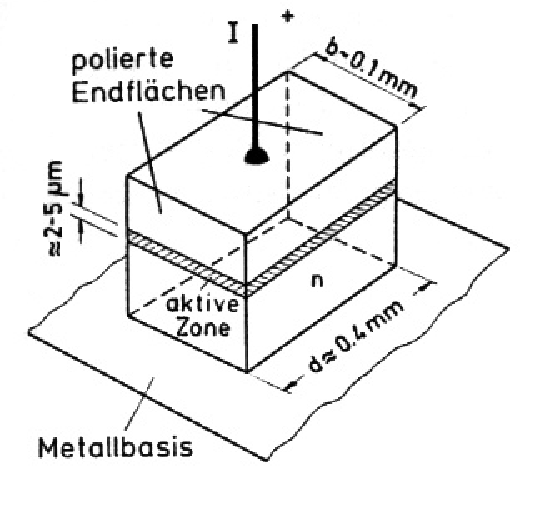
\includegraphics[width=0.5\textwidth]{graphics/laser}
	\caption{Setup of a typical diode laser~\cite{demtroed}}
	\label{fig:laser}
\end{figure}
The active medium is represented by a biased p-n-junction. If a voltage is applied (see figure \ref{fig:pn} right), the electrons are able to reach the boundary layer and recombine with the holes. Thus a photon of an energy correlated with the gap energy is emitted.
\begin{figure}[H]
	\centering
		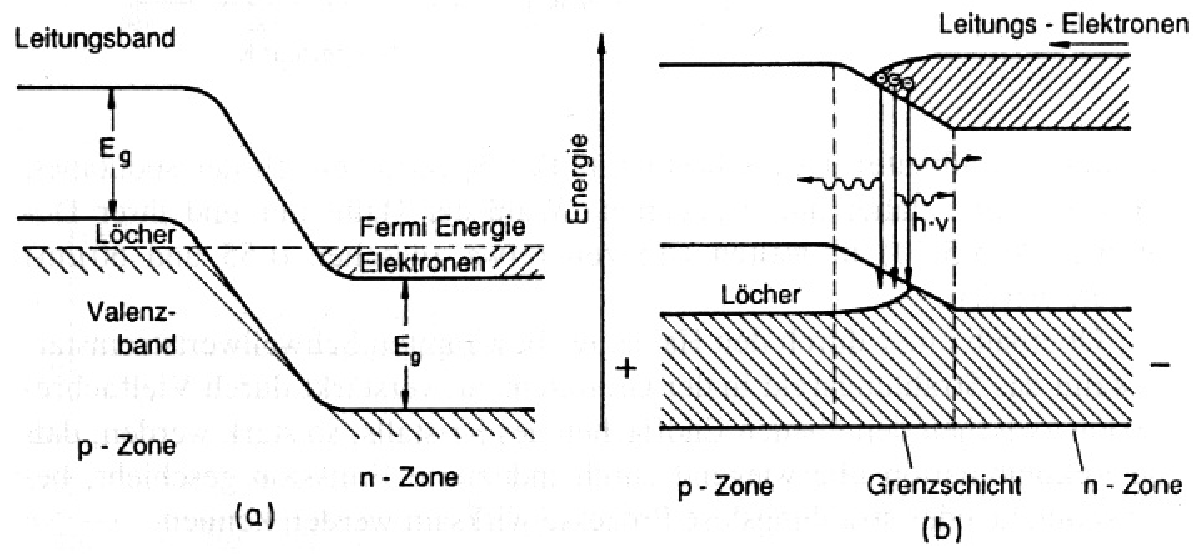
\includegraphics[width=0.9\textwidth]{graphics/pn}
	\caption{p-n-junction of a diode laser without (left) and with (right) applied voltage~\cite{demtroed}}
	\label{fig:pn}
\end{figure}
As the semiconductor crystal has a high refraction index (i.\ e.\ $n_{\mathrm{GaAs}} = 3.6$) in comparison to air ($n_{\mathrm{air}} \approx 1$), the reflectivity of the boundary surface of the crystal amounts to $R=[(n_{\mathrm{GaAs}}-1)/(n_{\mathrm{GaAs}}+1)]^2 = 0.32$. This can be optimized by polishing those surfaces. Therefore the orthogonal boundary layers of the crystal can indeed be used as a resonator.

Of course it is neccessary to adjust the power of the laser. For this the diode current has to be varied. But one has to consider that a threshold current $I_{\mathrm{thr}}$ exists, because the photons can be absorbed or scattered in the resonator which results in an energyloss. Only above this threshold the laser enters the linear working regime and is pumped efficently.

\subsection{Gaussian Beams}
Because laser beams have a finite beam size, it is neccessary to go beyond the model of plane waves and introduce so-called \textsc{gaussian} beams (see figure \ref{fig:gaussianbeams}). In this theoretical approach the beam has a \textsc{gaussian} intensity distribution perpendicular to the wave vector $\vec{k}$. Furthermore it is characterized by its beam radius $w(z)$ and the \textsc{Rayleigh}-length $z_0 = \pi w^2_0/\lambda$. For $|z| \leq z_0$ the beam is focussed and has its smallest radius $w_0$ which is called waist at $z=0$. For $z \ll z_0$ nearly plane waves propagate and for large $z$ one observes spherical wavefronts. Furthermore the angle of divergence can be derived to $\theta_{\mathrm{div}} = w_0/z_0 = \lambda/\pi w_0$.
\begin{figure}[H]
	\centering
		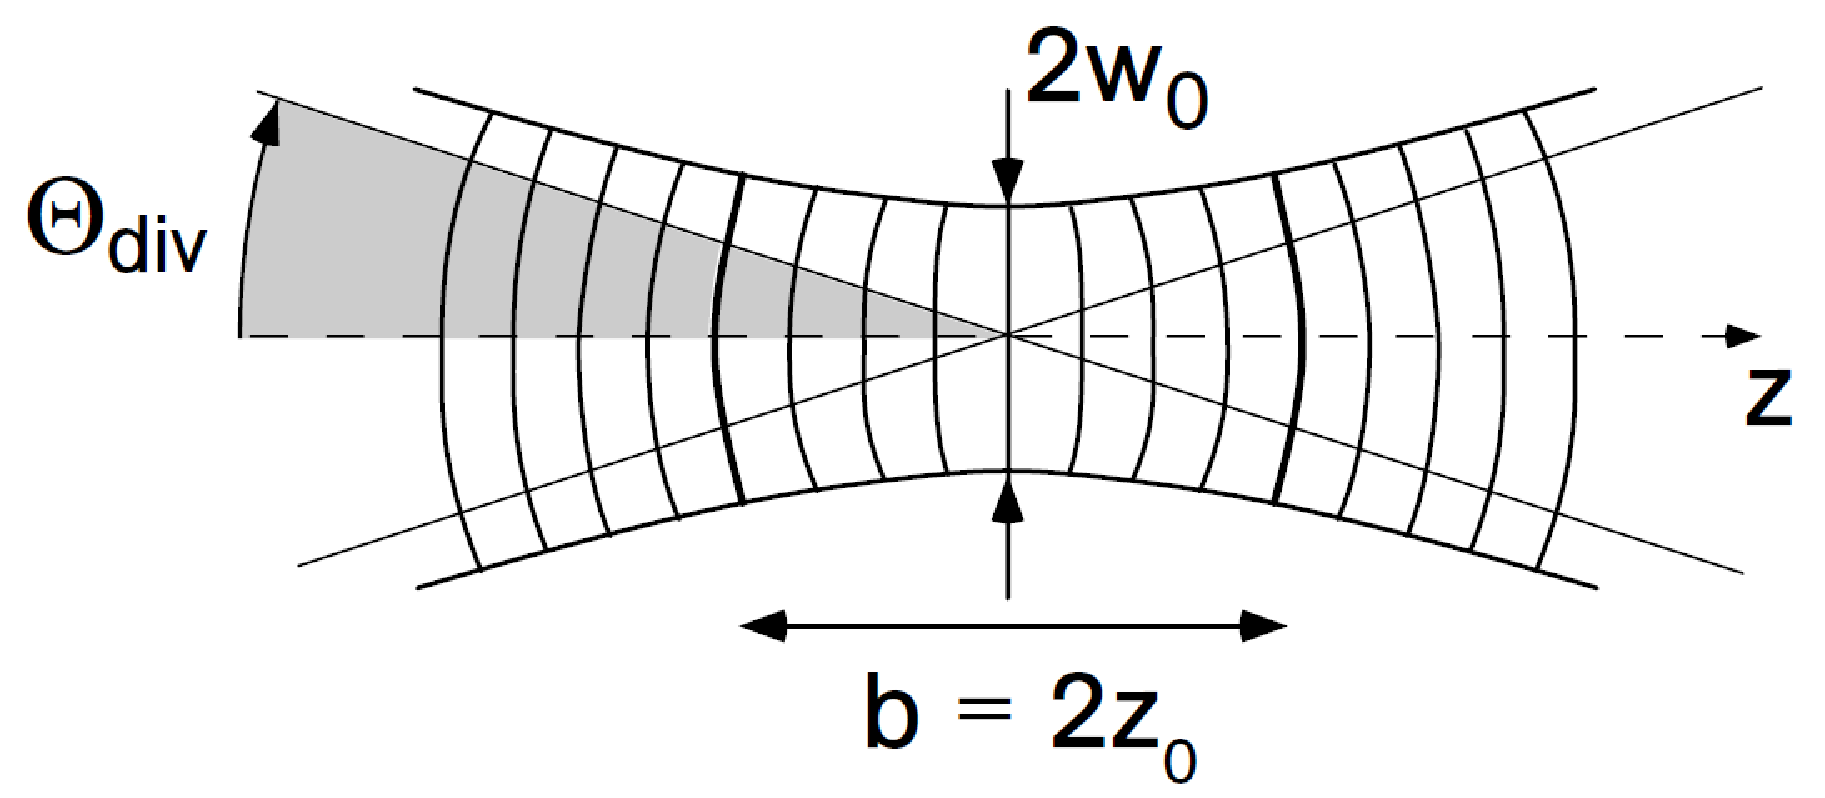
\includegraphics[width=0.8\textwidth]{graphics/gaussianbeams}
	\caption{Sketch of a \textsc{gaussian} beam~\cite{meschi}}
	\label{fig:gaussianbeams}
\end{figure}

\subsection{Birefringence}
\label{cha:bi}
If light propagates through an optical medium, the refraction index $n$ of this medium has to be considered. In addition crystals like $KNbO_3$ with anisotropic refraction indices because of anisotropic linkage forces exist. The symmetry axis (if there is one) of the crystal is called optical axis. 
\begin{figure}[H]
	\centering
		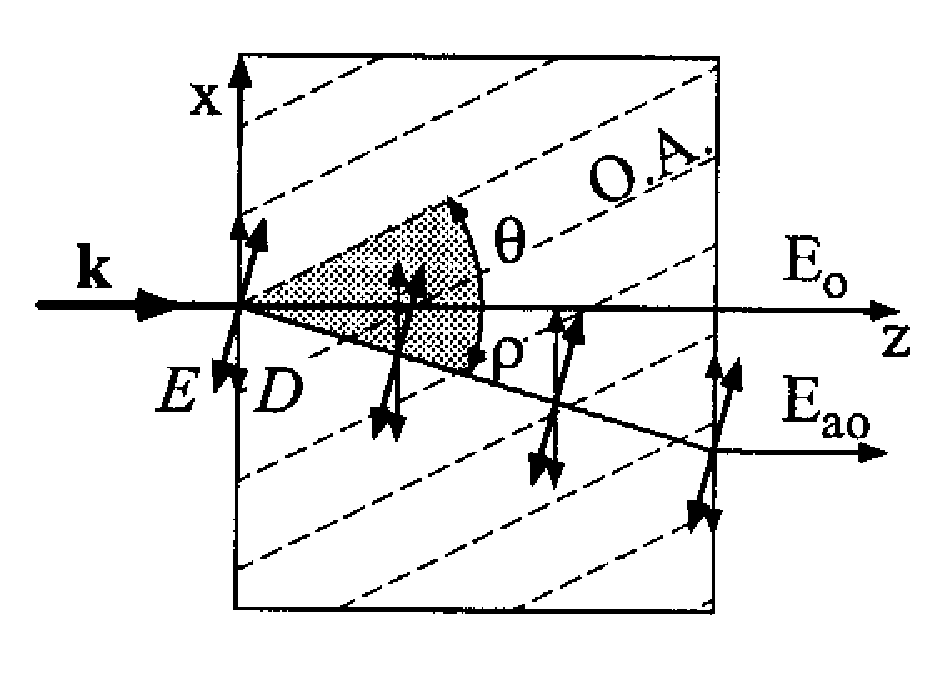
\includegraphics[width=0.7\textwidth]{graphics/brech}
	\caption{Walk off of the extraordinary beam~\cite{meschi}}
	\label{fig:brech}
\end{figure}
Due to this the polarisation $\vec{P}$ induced by the electromagnetic wave is not parallel to $\vec{E}$ anymore, which is explained thru the dielectric constant which turns into a three dimensional tensor. Therefore different polarized beams take different paths. The one which follows \textsc{Snellius'} law is called ordinary beam, while the other one experiencing a walk off (see also figure \ref{fig:brech}) is called extraordinary beam. Those beams have orthogonal polarisations. This effect of splitting an incoming beam is called birefringence and is used for example in $\lambda/2$-plates.


\subsection{Nonlinear Optics and Frequency Doubling}
The electrons of a crystal being exposed to electromagnetic waves are displaced from their position of rest. If these shifts are small, the restoring forces will depend linearly on the displacementamplitude, so indeed the \textsc{Hooke} law will apply. As a result the polarisation $\vec{P}$ is proportional to the present electric field $\vec{E}$. 

At high intensities of (coherent) light (i.\ e.\ laser light) though this approximation is not applicable anymore. Thereby higher orders of the \textsc{Taylor}-expansion of the polarisation also have to be considered. Assuming an isotropic medium $P_\mathrm{x} = \varepsilon_0 \left( \chi_1 E_\mathrm{x} + \chi_2 E^2_\mathrm{x} + \dots \right)$ holds for the x-component of the polarisation. Now one can insert the electric field of a monochromatic light wave and yields:
\begin{align}
P_\mathrm{x} &\approx \varepsilon_0 \left( \chi_1 E_0 \cos{\omega t} + \chi_2 E^2_0 \cos^2{\omega t} \right) \\
             &= \varepsilon_0 \left( \frac{1}{2} \chi_2 E^2_0 + \chi_1 E_0 \cos{\omega t} + \frac{1}{2} \chi_2 E^2_0 \cos{2 \omega t} \right) \ \ldotp
\end{align}
So indeed one gets an oscillation term at twice of the original frequency and a constant polarisation term in addition to the one for the linear approximation. With correct phase relation those second harmonic oscillations can add up to a macroscopic wave. But in general the phases do not match due to dispersion at different frequencies. To obtain phase matching do the following considerations.

Assuming plane waves and constant intensity $I_\mathrm{f}$ of the fundamental wave within a crystal of length $L$ the output intensity of the second harmonic $I_\mathrm{sh}$ after the crystal is given by:
\begin{align}
I_{\mathrm{sh}}\propto \, L^2 I^2_{\mathrm{f}} \left( \frac{\sin{\Delta k \frac{L}{2}}}{\Delta k \frac{L}{2}} \right)^2 \ ,
\end{align}
whereas $\Delta k = k(2\omega) - 2 k(\omega) = \frac{2\omega}{v_\mathrm{sh}} - 2 \frac{\omega}{v_\mathrm{f}} = \frac{2\omega}{c} \left( n(2\omega) - n(\omega) \right)$ is the phase mismatch. At minimal mismatch the output intensity of the second harmonic reaches its maximum due to maximal constructive interference, therefore the phase matching condition reads:
\begin{align}
\Delta k = 0 \hspace{1cm} \Leftrightarrow \hspace{1cm} n(2\omega) = n(\omega) \ \ldotp
\end{align}
On account of that nonlinear crystals have to be used, because such a phase matching is not possible with normally dispersive media. Indeed there $n(2\omega) > n(\omega)$ always holds. In anisotropic crystals though the refractive index of the second harmonic can be lowered for example by using the second harmonic as the extraordinary beam.

For this the angle between the incident wave and the optical axis is adjusted such that the above condition holds. This method is called \emph{angle tuning}. But there is a problem with this approach. Of course as written in section \ref{cha:bi} the extraordinary beam experiences a walk off for $\theta \neq 0, \pi/2$. This is problematic because the beams should overlap behind the crystal to obtain an interference pattern. Therefore one uses \emph{temperature tuning}. This furthermore also allows a high conversion efficiency into the second harmonic, which improves the intensity.


\subsection{Coherence}
Coherence is a measure of the phase correlation of wavefronts. Two waves are called coherent, if roughly speaking their phase difference is constant within a relevant range. Indeed coherence is neccessary for interference. One distinguishes between time coherence and spatial coherence, but for means of brevity we will not discuss this further.

\subsection{Optical Grating}
A grating is used to create an interference pattern on a screen via illuminating it with coherent light. The maxima obtain the relation $\sin{\alpha} = n \lambda/g$, whereas $\alpha$ is the angle of diffraction of the maximum of $n^{\mathrm{th}}$ order, $\lambda$ is the wavelength of the light and $g$ the grating constant.

The spectral resolution of such a grating amounts to $\lambda/\Delta\lambda = N n$, where $N$ is the number of illuminated slits, so indeed one can improve the resolution by illuminating the grating properly.

\subsection{Michelson Interferometer}
The \textsc{Michelson} interferometer is a very common configuration for optical interferometry and was invented by Albert Abraham Michelson. 
\begin{figure}[H]
	\centering
		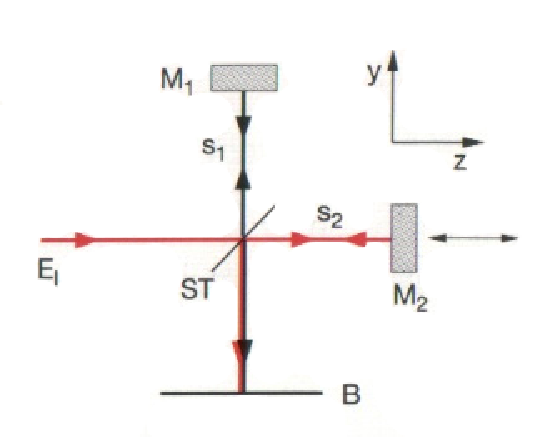
\includegraphics[width=0.6\textwidth]{graphics/michelson}
	\caption{\textsc{Michelson} interferometer~\cite{demtroed2}}
	\label{fig:michelson}
\end{figure}
As depicted above the incoming beam hits a beam splitter, so one reflects off, propagates to the top mirror and then reflects back, goes through the semi-transparent mirror again and reaches the detector. The other beam first passes the beam splitter and hits the mirror on the right. It is then reflected back and reflects off the beam splitter into the detector. So both beams travel indeed along different paths. As the right mirror can be displaced on an optical bank one can change the distance $s_2$ and therefore change the relative path difference of the two beams. This results in a phase difference $\Delta \phi = 2\pi (s_1-s_2)/\lambda$.



\section{Experimentation and Analysis}
\subsection{Diode Laser and power measurements}\label{ana_laserpower}
To get familiar with the laser we first examine the laser power depencence on the input current. Therefore we put a gauged photodiode in front of the laser and record the laser power for different values of the input current. Do avoid the photodiode to leave its 'linear range' we put an attenuator in front of it. The measured values are displayed in table \ref{tab:ana_laserpower_att} in the appendix. In order to gauge the attenuator we also recorded some values in the range between threshold current and an output of $\unit[50]{\mu W}$ without using the attenuator. These values are displayed in table \ref{tab:ana_laserpower_woatt} in the appendix.

Figure \ref{fig:ana_laser_watt} and \ref{fig:ana_laser_woatt} show plots of laser power with and without the attenuator as well as linear fits to the data taken above the threshold current. The fit results read:
\begin{align}
P_\textrm{att}(I) &= b_\textrm{att} + m_\textrm{att} \,\cdotp\, I = \unit[(-33.8 \pm 0.14)]{\mu W} + \unit[(0.574 \pm 0.002
)]{\frac{\mu W}{mA}}\,\cdotp\, I\\
P_\textrm{real}(I) &= b_\textrm{real} + m_\textrm{real} \,\cdotp\, I =\unit[(-36 \pm 1.5)]{mW} + \unit[(0.60 \pm 0.02
)]{\frac{mW}{mA}}\,\cdotp\, I
\end{align}
The ratio of the gradients yields the attenuation:
\begin{align}
\alpha = \unit[(1049 \pm 36)]{}
\end{align}
where the error is calculated via
\begin{align*}
\Delta \alpha = \sqrt{\left(\frac{\Delta m_\textrm{att}}{m_\textrm{real}}\right)^2 + \left(\frac{m_\textrm{att}}{m^2_\textrm{real}}\Delta m_\textrm{real}\right)^2}
\end{align*}
\begin{figure}[H]
\begin{floatrow}
\ffigbox[0.5\textwidth]{}
{
\resizebox{0.5\textwidth}{!}{
%	\begin{tikzpicture}[gnuplot]
%% generated with GNUPLOT 4.4p0 (Lua 5.1.4; terminal rev. 97, script rev. 96a)
%% 29.04.2010 21:37:31
\gpcolor{gp lt color border}
\gpsetlinetype{gp lt border}
\gpsetlinewidth{1.00}
\draw[gp path] (1.688,1.337)--(1.868,1.337);
\draw[gp path] (12.039,1.337)--(11.859,1.337);
\node[gp node right] at (1.504,1.337) { 0};
\draw[gp path] (1.688,3.098)--(1.868,3.098);
\draw[gp path] (12.039,3.098)--(11.859,3.098);
\node[gp node right] at (1.504,3.098) { 50};
\draw[gp path] (1.688,4.859)--(1.868,4.859);
\draw[gp path] (12.039,4.859)--(11.859,4.859);
\node[gp node right] at (1.504,4.859) { 100};
\draw[gp path] (1.688,6.620)--(1.868,6.620);
\draw[gp path] (12.039,6.620)--(11.859,6.620);
\node[gp node right] at (1.504,6.620) { 150};
\draw[gp path] (1.688,8.381)--(1.868,8.381);
\draw[gp path] (12.039,8.381)--(11.859,8.381);
\node[gp node right] at (1.504,8.381) { 200};
\draw[gp path] (1.688,0.985)--(1.688,1.165);
\draw[gp path] (1.688,8.381)--(1.688,8.201);
\node[gp node center] at (1.688,0.677) { 0};
\draw[gp path] (3.413,0.985)--(3.413,1.165);
\draw[gp path] (3.413,8.381)--(3.413,8.201);
\node[gp node center] at (3.413,0.677) { 50};
\draw[gp path] (5.138,0.985)--(5.138,1.165);
\draw[gp path] (5.138,8.381)--(5.138,8.201);
\node[gp node center] at (5.138,0.677) { 100};
\draw[gp path] (6.863,0.985)--(6.863,1.165);
\draw[gp path] (6.863,8.381)--(6.863,8.201);
\node[gp node center] at (6.863,0.677) { 150};
\draw[gp path] (8.589,0.985)--(8.589,1.165);
\draw[gp path] (8.589,8.381)--(8.589,8.201);
\node[gp node center] at (8.589,0.677) { 200};
\draw[gp path] (10.314,0.985)--(10.314,1.165);
\draw[gp path] (10.314,8.381)--(10.314,8.201);
\node[gp node center] at (10.314,0.677) { 250};
\draw[gp path] (12.039,0.985)--(12.039,1.165);
\draw[gp path] (12.039,8.381)--(12.039,8.201);
\node[gp node center] at (12.039,0.677) { 300};
\draw[gp path] (1.688,8.381)--(1.688,0.985)--(12.039,0.985)--(12.039,8.381)--cycle;
\node[gp node center,rotate=-270] at (0.430,4.683) {Laser power [$\mu$W]};
\node[gp node center] at (6.863,0.215) {Input current [mA]};
\node[gp node right] at (10.571,8.047) {Measured Data};
\gpcolor{gp lt color 0}
\gpsetlinetype{gp lt plot 0}
\draw[gp path] (10.755,8.047)--(11.671,8.047);
\draw[gp path] (10.755,8.137)--(10.755,7.957);
\draw[gp path] (11.671,8.137)--(11.671,7.957);
\draw[gp path] (1.633,1.337)--(1.813,1.337);
\draw[gp path] (1.633,1.337)--(1.813,1.337);
\draw[gp path] (1.978,1.337)--(2.158,1.337);
\draw[gp path] (1.978,1.337)--(2.158,1.337);
\draw[gp path] (2.288,1.337)--(2.468,1.337);
\draw[gp path] (2.288,1.337)--(2.468,1.337);
\draw[gp path] (2.633,1.337)--(2.813,1.337);
\draw[gp path] (2.633,1.337)--(2.813,1.337);
\draw[gp path] (2.978,1.337)--(3.158,1.337);
\draw[gp path] (2.978,1.337)--(3.158,1.337);
\draw[gp path] (3.151,1.337)--(3.331,1.337);
\draw[gp path] (3.151,1.337)--(3.331,1.337);
\draw[gp path] (3.323,1.337)--(3.503,1.337);
\draw[gp path] (3.323,1.337)--(3.503,1.337);
\draw[gp path] (3.496,1.337)--(3.676,1.337);
\draw[gp path] (3.496,1.337)--(3.676,1.337);
\draw[gp path] (3.668,1.359)--(3.848,1.359);
\draw[gp path] (3.668,1.359)--(3.848,1.359);
\draw[gp path] (3.931,1.454)--(3.931,1.455);
\draw[gp path] (3.841,1.454)--(4.021,1.454);
\draw[gp path] (3.841,1.455)--(4.021,1.455);
\draw[gp path] (4.103,1.560)--(4.103,1.561);
\draw[gp path] (4.013,1.560)--(4.193,1.560);
\draw[gp path] (4.013,1.561)--(4.193,1.561);
\draw[gp path] (4.276,1.674)--(4.276,1.675);
\draw[gp path] (4.186,1.674)--(4.366,1.674);
\draw[gp path] (4.186,1.675)--(4.366,1.675);
\draw[gp path] (4.448,1.788)--(4.448,1.795);
\draw[gp path] (4.358,1.788)--(4.538,1.788);
\draw[gp path] (4.358,1.795)--(4.538,1.795);
\draw[gp path] (4.793,1.915)--(4.793,1.922);
\draw[gp path] (4.703,1.915)--(4.883,1.915);
\draw[gp path] (4.703,1.922)--(4.883,1.922);
\draw[gp path] (5.138,2.211)--(5.138,2.218);
\draw[gp path] (5.048,2.211)--(5.228,2.211);
\draw[gp path] (5.048,2.218)--(5.228,2.218);
\draw[gp path] (5.483,2.334)--(5.483,2.341);
\draw[gp path] (5.393,2.334)--(5.573,2.334);
\draw[gp path] (5.393,2.341)--(5.573,2.341);
\draw[gp path] (5.828,2.580)--(5.828,2.587);
\draw[gp path] (5.738,2.580)--(5.918,2.580);
\draw[gp path] (5.738,2.587)--(5.918,2.587);
\draw[gp path] (6.173,2.778)--(6.173,2.785);
\draw[gp path] (6.083,2.778)--(6.263,2.778);
\draw[gp path] (6.083,2.785)--(6.263,2.785);
\draw[gp path] (6.518,2.954)--(6.518,2.961);
\draw[gp path] (6.428,2.954)--(6.608,2.954);
\draw[gp path] (6.428,2.961)--(6.608,2.961);
\draw[gp path] (6.863,3.165)--(6.863,3.172);
\draw[gp path] (6.773,3.165)--(6.953,3.165);
\draw[gp path] (6.773,3.172)--(6.953,3.172);
\draw[gp path] (7.209,3.394)--(7.209,3.401);
\draw[gp path] (7.119,3.394)--(7.299,3.394);
\draw[gp path] (7.119,3.401)--(7.299,3.401);
\draw[gp path] (7.554,3.588)--(7.554,3.595);
\draw[gp path] (7.464,3.588)--(7.644,3.588);
\draw[gp path] (7.464,3.595)--(7.644,3.595);
\draw[gp path] (7.899,3.792)--(7.899,3.799);
\draw[gp path] (7.809,3.792)--(7.989,3.792);
\draw[gp path] (7.809,3.799)--(7.989,3.799);
\draw[gp path] (8.244,4.000)--(8.244,4.007);
\draw[gp path] (8.154,4.000)--(8.334,4.000);
\draw[gp path] (8.154,4.007)--(8.334,4.007);
\draw[gp path] (8.589,4.148)--(8.589,4.155);
\draw[gp path] (8.499,4.148)--(8.679,4.148);
\draw[gp path] (8.499,4.155)--(8.679,4.155);
\draw[gp path] (8.934,4.363)--(8.934,4.370);
\draw[gp path] (8.844,4.363)--(9.024,4.363);
\draw[gp path] (8.844,4.370)--(9.024,4.370);
\draw[gp path] (9.279,4.514)--(9.279,4.521);
\draw[gp path] (9.189,4.514)--(9.369,4.514);
\draw[gp path] (9.189,4.521)--(9.369,4.521);
\draw[gp path] (9.624,4.785)--(9.624,4.792);
\draw[gp path] (9.534,4.785)--(9.714,4.785);
\draw[gp path] (9.534,4.792)--(9.714,4.792);
\draw[gp path] (9.969,4.965)--(9.969,5.035);
\draw[gp path] (9.879,4.965)--(10.059,4.965);
\draw[gp path] (9.879,5.035)--(10.059,5.035);
\draw[gp path] (10.314,5.247)--(10.314,5.317);
\draw[gp path] (10.224,5.247)--(10.404,5.247);
\draw[gp path] (10.224,5.317)--(10.404,5.317);
\draw[gp path] (10.659,5.317)--(10.659,5.387);
\draw[gp path] (10.569,5.317)--(10.749,5.317);
\draw[gp path] (10.569,5.387)--(10.749,5.387);
\draw[gp path] (11.004,5.669)--(11.004,5.740);
\draw[gp path] (10.914,5.669)--(11.094,5.669);
\draw[gp path] (10.914,5.740)--(11.094,5.740);
\draw[gp path] (11.349,5.740)--(11.349,5.810);
\draw[gp path] (11.259,5.740)--(11.439,5.740);
\draw[gp path] (11.259,5.810)--(11.439,5.810);
\draw[gp path] (1.705,1.337)--(1.740,1.337);
\draw[gp path] (1.705,1.247)--(1.705,1.427);
\draw[gp path] (1.740,1.247)--(1.740,1.427);
\draw[gp path] (2.050,1.337)--(2.085,1.337);
\draw[gp path] (2.050,1.247)--(2.050,1.427);
\draw[gp path] (2.085,1.247)--(2.085,1.427);
\draw[gp path] (2.361,1.337)--(2.395,1.337);
\draw[gp path] (2.361,1.247)--(2.361,1.427);
\draw[gp path] (2.395,1.247)--(2.395,1.427);
\draw[gp path] (2.706,1.337)--(2.740,1.337);
\draw[gp path] (2.706,1.247)--(2.706,1.427);
\draw[gp path] (2.740,1.247)--(2.740,1.427);
\draw[gp path] (3.051,1.337)--(3.085,1.337);
\draw[gp path] (3.051,1.247)--(3.051,1.427);
\draw[gp path] (3.085,1.247)--(3.085,1.427);
\draw[gp path] (3.223,1.337)--(3.258,1.337);
\draw[gp path] (3.223,1.247)--(3.223,1.427);
\draw[gp path] (3.258,1.247)--(3.258,1.427);
\draw[gp path] (3.396,1.337)--(3.430,1.337);
\draw[gp path] (3.396,1.247)--(3.396,1.427);
\draw[gp path] (3.430,1.247)--(3.430,1.427);
\draw[gp path] (3.568,1.337)--(3.603,1.337);
\draw[gp path] (3.568,1.247)--(3.568,1.427);
\draw[gp path] (3.603,1.247)--(3.603,1.427);
\draw[gp path] (3.741,1.359)--(3.775,1.359);
\draw[gp path] (3.741,1.269)--(3.741,1.449);
\draw[gp path] (3.775,1.269)--(3.775,1.449);
\draw[gp path] (3.913,1.454)--(3.948,1.454);
\draw[gp path] (3.913,1.364)--(3.913,1.544);
\draw[gp path] (3.948,1.364)--(3.948,1.544);
\draw[gp path] (4.086,1.560)--(4.120,1.560);
\draw[gp path] (4.086,1.470)--(4.086,1.650);
\draw[gp path] (4.120,1.470)--(4.120,1.650);
\draw[gp path] (4.258,1.675)--(4.293,1.675);
\draw[gp path] (4.258,1.585)--(4.258,1.765);
\draw[gp path] (4.293,1.585)--(4.293,1.765);
\draw[gp path] (4.431,1.792)--(4.466,1.792);
\draw[gp path] (4.431,1.702)--(4.431,1.882);
\draw[gp path] (4.466,1.702)--(4.466,1.882);
\draw[gp path] (4.776,1.918)--(4.811,1.918);
\draw[gp path] (4.776,1.828)--(4.776,2.008);
\draw[gp path] (4.811,1.828)--(4.811,2.008);
\draw[gp path] (5.121,2.214)--(5.156,2.214);
\draw[gp path] (5.121,2.124)--(5.121,2.304);
\draw[gp path] (5.156,2.124)--(5.156,2.304);
\draw[gp path] (5.466,2.337)--(5.501,2.337);
\draw[gp path] (5.466,2.247)--(5.466,2.427);
\draw[gp path] (5.501,2.247)--(5.501,2.427);
\draw[gp path] (5.811,2.584)--(5.846,2.584);
\draw[gp path] (5.811,2.494)--(5.811,2.674);
\draw[gp path] (5.846,2.494)--(5.846,2.674);
\draw[gp path] (6.156,2.781)--(6.191,2.781);
\draw[gp path] (6.156,2.691)--(6.156,2.871);
\draw[gp path] (6.191,2.691)--(6.191,2.871);
\draw[gp path] (6.501,2.957)--(6.536,2.957);
\draw[gp path] (6.501,2.867)--(6.501,3.047);
\draw[gp path] (6.536,2.867)--(6.536,3.047);
\draw[gp path] (6.846,3.169)--(6.881,3.169);
\draw[gp path] (6.846,3.079)--(6.846,3.259);
\draw[gp path] (6.881,3.079)--(6.881,3.259);
\draw[gp path] (7.191,3.398)--(7.226,3.398);
\draw[gp path] (7.191,3.308)--(7.191,3.488);
\draw[gp path] (7.226,3.308)--(7.226,3.488);
\draw[gp path] (7.536,3.591)--(7.571,3.591);
\draw[gp path] (7.536,3.501)--(7.536,3.681);
\draw[gp path] (7.571,3.501)--(7.571,3.681);
\draw[gp path] (7.881,3.795)--(7.916,3.795);
\draw[gp path] (7.881,3.705)--(7.881,3.885);
\draw[gp path] (7.916,3.705)--(7.916,3.885);
\draw[gp path] (8.226,4.003)--(8.261,4.003);
\draw[gp path] (8.226,3.913)--(8.226,4.093);
\draw[gp path] (8.261,3.913)--(8.261,4.093);
\draw[gp path] (8.571,4.151)--(8.606,4.151);
\draw[gp path] (8.571,4.061)--(8.571,4.241);
\draw[gp path] (8.606,4.061)--(8.606,4.241);
\draw[gp path] (8.916,4.366)--(8.951,4.366);
\draw[gp path] (8.916,4.276)--(8.916,4.456);
\draw[gp path] (8.951,4.276)--(8.951,4.456);
\draw[gp path] (9.261,4.517)--(9.296,4.517);
\draw[gp path] (9.261,4.427)--(9.261,4.607);
\draw[gp path] (9.296,4.427)--(9.296,4.607);
\draw[gp path] (9.607,4.789)--(9.641,4.789);
\draw[gp path] (9.607,4.699)--(9.607,4.879);
\draw[gp path] (9.641,4.699)--(9.641,4.879);
\draw[gp path] (9.952,5.000)--(9.986,5.000);
\draw[gp path] (9.952,4.910)--(9.952,5.090);
\draw[gp path] (9.986,4.910)--(9.986,5.090);
\draw[gp path] (10.297,5.282)--(10.331,5.282);
\draw[gp path] (10.297,5.192)--(10.297,5.372);
\draw[gp path] (10.331,5.192)--(10.331,5.372);
\draw[gp path] (10.642,5.352)--(10.676,5.352);
\draw[gp path] (10.642,5.262)--(10.642,5.442);
\draw[gp path] (10.676,5.262)--(10.676,5.442);
\draw[gp path] (10.987,5.704)--(11.021,5.704);
\draw[gp path] (10.987,5.614)--(10.987,5.794);
\draw[gp path] (11.021,5.614)--(11.021,5.794);
\draw[gp path] (11.332,5.775)--(11.366,5.775);
\draw[gp path] (11.332,5.685)--(11.332,5.865);
\draw[gp path] (11.366,5.685)--(11.366,5.865);
\gpsetpointsize{4.00}
\gppoint{gp mark 1}{(1.723,1.337)}
\gppoint{gp mark 1}{(2.068,1.337)}
\gppoint{gp mark 1}{(2.378,1.337)}
\gppoint{gp mark 1}{(2.723,1.337)}
\gppoint{gp mark 1}{(3.068,1.337)}
\gppoint{gp mark 1}{(3.241,1.337)}
\gppoint{gp mark 1}{(3.413,1.337)}
\gppoint{gp mark 1}{(3.586,1.337)}
\gppoint{gp mark 1}{(3.758,1.359)}
\gppoint{gp mark 1}{(3.931,1.454)}
\gppoint{gp mark 1}{(4.103,1.560)}
\gppoint{gp mark 1}{(4.276,1.675)}
\gppoint{gp mark 1}{(4.448,1.792)}
\gppoint{gp mark 1}{(4.793,1.918)}
\gppoint{gp mark 1}{(5.138,2.214)}
\gppoint{gp mark 1}{(5.483,2.337)}
\gppoint{gp mark 1}{(5.828,2.584)}
\gppoint{gp mark 1}{(6.173,2.781)}
\gppoint{gp mark 1}{(6.518,2.957)}
\gppoint{gp mark 1}{(6.863,3.169)}
\gppoint{gp mark 1}{(7.209,3.398)}
\gppoint{gp mark 1}{(7.554,3.591)}
\gppoint{gp mark 1}{(7.899,3.795)}
\gppoint{gp mark 1}{(8.244,4.003)}
\gppoint{gp mark 1}{(8.589,4.151)}
\gppoint{gp mark 1}{(8.934,4.366)}
\gppoint{gp mark 1}{(9.279,4.517)}
\gppoint{gp mark 1}{(9.624,4.789)}
\gppoint{gp mark 1}{(9.969,5.000)}
\gppoint{gp mark 1}{(10.314,5.282)}
\gppoint{gp mark 1}{(10.659,5.352)}
\gppoint{gp mark 1}{(11.004,5.704)}
\gppoint{gp mark 1}{(11.349,5.775)}
\gppoint{gp mark 1}{(11.213,8.047)}
\gpcolor{gp lt color border}
\node[gp node right] at (10.571,7.739) {Fit};
\gpsetlinetype{gp lt border}
\draw[gp path] (10.755,7.739)--(11.671,7.739);
\draw[gp path] (3.120,0.985)--(3.152,1.004)--(3.256,1.065)--(3.361,1.126)--(3.465,1.187)%
  --(3.570,1.249)--(3.675,1.310)--(3.779,1.371)--(3.884,1.432)--(3.988,1.493)--(4.093,1.555)%
  --(4.197,1.616)--(4.302,1.677)--(4.406,1.738)--(4.511,1.800)--(4.616,1.861)--(4.720,1.922)%
  --(4.825,1.983)--(4.929,2.045)--(5.034,2.106)--(5.138,2.167)--(5.243,2.228)--(5.347,2.289)%
  --(5.452,2.351)--(5.557,2.412)--(5.661,2.473)--(5.766,2.534)--(5.870,2.596)--(5.975,2.657)%
  --(6.079,2.718)--(6.184,2.779)--(6.288,2.841)--(6.393,2.902)--(6.498,2.963)--(6.602,3.024)%
  --(6.707,3.086)--(6.811,3.147)--(6.916,3.208)--(7.020,3.269)--(7.125,3.330)--(7.229,3.392)%
  --(7.334,3.453)--(7.439,3.514)--(7.543,3.575)--(7.648,3.637)--(7.752,3.698)--(7.857,3.759)%
  --(7.961,3.820)--(8.066,3.882)--(8.170,3.943)--(8.275,4.004)--(8.380,4.065)--(8.484,4.127)%
  --(8.589,4.188)--(8.693,4.249)--(8.798,4.310)--(8.902,4.371)--(9.007,4.433)--(9.111,4.494)%
  --(9.216,4.555)--(9.321,4.616)--(9.425,4.678)--(9.530,4.739)--(9.634,4.800)--(9.739,4.861)%
  --(9.843,4.923)--(9.948,4.984)--(10.052,5.045)--(10.157,5.106)--(10.262,5.167)--(10.366,5.229)%
  --(10.471,5.290)--(10.575,5.351)--(10.680,5.412)--(10.784,5.474)--(10.889,5.535)--(10.993,5.596)%
  --(11.098,5.657)--(11.203,5.719)--(11.307,5.780)--(11.412,5.841)--(11.516,5.902)--(11.621,5.964)%
  --(11.725,6.025)--(11.830,6.086)--(11.934,6.147)--(12.039,6.208);
\draw[gp path] (1.688,8.381)--(1.688,0.985)--(12.039,0.985)--(12.039,8.381)--cycle;
%% coordinates of the plot area
\gpdefrectangularnode{gp plot 1}{\pgfpoint{1.688cm}{0.985cm}}{\pgfpoint{12.039cm}{8.381cm}}
\end{tikzpicture}
%% gnuplot variables

}
	\caption{Attenuated laser output power versus input current and corresponding linear fit}
	\label{fig:ana_laser_watt}
}
\ffigbox[0.5\textwidth]{}
{
\resizebox{0.5\textwidth}{!}{
	%\begin{tikzpicture}[gnuplot]
%% generated with GNUPLOT 4.4p0 (Lua 5.1.4; terminal rev. 97, script rev. 96a)
%% 29.04.2010 21:37:32
\gpcolor{gp lt color border}
\gpsetlinetype{gp lt border}
\gpsetlinewidth{1.00}
\draw[gp path] (1.504,0.985)--(1.684,0.985);
\draw[gp path] (12.039,0.985)--(11.859,0.985);
\node[gp node right] at (1.320,0.985) { 0};
\draw[gp path] (1.504,2.218)--(1.684,2.218);
\draw[gp path] (12.039,2.218)--(11.859,2.218);
\node[gp node right] at (1.320,2.218) { 5};
\draw[gp path] (1.504,3.450)--(1.684,3.450);
\draw[gp path] (12.039,3.450)--(11.859,3.450);
\node[gp node right] at (1.320,3.450) { 10};
\draw[gp path] (1.504,4.683)--(1.684,4.683);
\draw[gp path] (12.039,4.683)--(11.859,4.683);
\node[gp node right] at (1.320,4.683) { 15};
\draw[gp path] (1.504,5.916)--(1.684,5.916);
\draw[gp path] (12.039,5.916)--(11.859,5.916);
\node[gp node right] at (1.320,5.916) { 20};
\draw[gp path] (1.504,7.148)--(1.684,7.148);
\draw[gp path] (12.039,7.148)--(11.859,7.148);
\node[gp node right] at (1.320,7.148) { 25};
\draw[gp path] (1.504,8.381)--(1.684,8.381);
\draw[gp path] (12.039,8.381)--(11.859,8.381);
\node[gp node right] at (1.320,8.381) { 30};
\draw[gp path] (2.557,0.985)--(2.557,1.165);
\draw[gp path] (2.557,8.381)--(2.557,8.201);
\node[gp node center] at (2.557,0.677) { 60};
\draw[gp path] (4.664,0.985)--(4.664,1.165);
\draw[gp path] (4.664,8.381)--(4.664,8.201);
\node[gp node center] at (4.664,0.677) { 70};
\draw[gp path] (6.771,0.985)--(6.771,1.165);
\draw[gp path] (6.771,8.381)--(6.771,8.201);
\node[gp node center] at (6.771,0.677) { 80};
\draw[gp path] (8.878,0.985)--(8.878,1.165);
\draw[gp path] (8.878,8.381)--(8.878,8.201);
\node[gp node center] at (8.878,0.677) { 90};
\draw[gp path] (10.985,0.985)--(10.985,1.165);
\draw[gp path] (10.985,8.381)--(10.985,8.201);
\node[gp node center] at (10.985,0.677) { 100};
\draw[gp path] (1.504,8.381)--(1.504,0.985)--(12.039,0.985)--(12.039,8.381)--cycle;
\node[gp node center,rotate=-270] at (0.430,4.683) {Laser power [mW]};
\node[gp node center] at (6.771,0.215) {Input current [mA]};
\node[gp node right] at (10.571,8.047) {Measured Data};
\gpcolor{gp lt color 0}
\gpsetlinetype{gp lt plot 0}
\draw[gp path] (10.755,8.047)--(11.671,8.047);
\draw[gp path] (10.755,8.137)--(10.755,7.957);
\draw[gp path] (11.671,8.137)--(11.671,7.957);
\draw[gp path] (2.557,1.142)--(2.557,1.146);
\draw[gp path] (2.467,1.142)--(2.647,1.142);
\draw[gp path] (2.467,1.146)--(2.647,1.146);
\draw[gp path] (3.611,1.739)--(3.611,1.744);
\draw[gp path] (3.521,1.739)--(3.701,1.739);
\draw[gp path] (3.521,1.744)--(3.701,1.744);
\draw[gp path] (4.664,2.353)--(4.664,2.358);
\draw[gp path] (4.574,2.353)--(4.754,2.353);
\draw[gp path] (4.574,2.358)--(4.754,2.358);
\draw[gp path] (5.718,3.221)--(5.718,3.226);
\draw[gp path] (5.628,3.221)--(5.808,3.221);
\draw[gp path] (5.628,3.226)--(5.808,3.226);
\draw[gp path] (6.771,3.968)--(6.771,4.017);
\draw[gp path] (6.681,3.968)--(6.861,3.968);
\draw[gp path] (6.681,4.017)--(6.861,4.017);
\draw[gp path] (7.825,4.535)--(7.825,4.584);
\draw[gp path] (7.735,4.535)--(7.915,4.535);
\draw[gp path] (7.735,4.584)--(7.915,4.584);
\draw[gp path] (8.878,5.250)--(8.878,5.299);
\draw[gp path] (8.788,5.250)--(8.968,5.250);
\draw[gp path] (8.788,5.299)--(8.968,5.299);
\draw[gp path] (9.932,6.236)--(9.932,6.285);
\draw[gp path] (9.842,6.236)--(10.022,6.236);
\draw[gp path] (9.842,6.285)--(10.022,6.285);
\draw[gp path] (10.985,6.926)--(10.985,6.976);
\draw[gp path] (10.895,6.926)--(11.075,6.926);
\draw[gp path] (10.895,6.976)--(11.075,6.976);
\draw[gp path] (2.452,1.144)--(2.663,1.144);
\draw[gp path] (2.452,1.054)--(2.452,1.234);
\draw[gp path] (2.663,1.054)--(2.663,1.234);
\draw[gp path] (3.506,1.742)--(3.716,1.742);
\draw[gp path] (3.506,1.652)--(3.506,1.832);
\draw[gp path] (3.716,1.652)--(3.716,1.832);
\draw[gp path] (4.559,2.356)--(4.770,2.356);
\draw[gp path] (4.559,2.266)--(4.559,2.446);
\draw[gp path] (4.770,2.266)--(4.770,2.446);
\draw[gp path] (5.613,3.224)--(5.823,3.224);
\draw[gp path] (5.613,3.134)--(5.613,3.314);
\draw[gp path] (5.823,3.134)--(5.823,3.314);
\draw[gp path] (6.666,3.993)--(6.877,3.993);
\draw[gp path] (6.666,3.903)--(6.666,4.083);
\draw[gp path] (6.877,3.903)--(6.877,4.083);
\draw[gp path] (7.720,4.560)--(7.930,4.560);
\draw[gp path] (7.720,4.470)--(7.720,4.650);
\draw[gp path] (7.930,4.470)--(7.930,4.650);
\draw[gp path] (8.773,5.275)--(8.984,5.275);
\draw[gp path] (8.773,5.185)--(8.773,5.365);
\draw[gp path] (8.984,5.185)--(8.984,5.365);
\draw[gp path] (9.827,6.261)--(10.037,6.261);
\draw[gp path] (9.827,6.171)--(9.827,6.351);
\draw[gp path] (10.037,6.171)--(10.037,6.351);
\draw[gp path] (10.880,6.951)--(11.091,6.951);
\draw[gp path] (10.880,6.861)--(10.880,7.041);
\draw[gp path] (11.091,6.861)--(11.091,7.041);
\gpsetpointsize{4.00}
\gppoint{gp mark 1}{(2.557,1.144)}
\gppoint{gp mark 1}{(3.611,1.742)}
\gppoint{gp mark 1}{(4.664,2.356)}
\gppoint{gp mark 1}{(5.718,3.224)}
\gppoint{gp mark 1}{(6.771,3.993)}
\gppoint{gp mark 1}{(7.825,4.560)}
\gppoint{gp mark 1}{(8.878,5.275)}
\gppoint{gp mark 1}{(9.932,6.261)}
\gppoint{gp mark 1}{(10.985,6.951)}
\gppoint{gp mark 1}{(11.213,8.047)}
\gpcolor{gp lt color border}
\node[gp node right] at (10.571,7.739) {Fit};
\gpsetlinetype{gp lt border}
\draw[gp path] (10.755,7.739)--(11.671,7.739);
\draw[gp path] (2.598,0.985)--(2.675,1.039)--(2.781,1.114)--(2.887,1.189)--(2.994,1.264)%
  --(3.100,1.339)--(3.207,1.414)--(3.313,1.489)--(3.419,1.564)--(3.526,1.639)--(3.632,1.714)%
  --(3.739,1.788)--(3.845,1.863)--(3.952,1.938)--(4.058,2.013)--(4.164,2.088)--(4.271,2.163)%
  --(4.377,2.238)--(4.484,2.313)--(4.590,2.388)--(4.696,2.463)--(4.803,2.538)--(4.909,2.613)%
  --(5.016,2.688)--(5.122,2.763)--(5.228,2.838)--(5.335,2.912)--(5.441,2.987)--(5.548,3.062)%
  --(5.654,3.137)--(5.761,3.212)--(5.867,3.287)--(5.973,3.362)--(6.080,3.437)--(6.186,3.512)%
  --(6.293,3.587)--(6.399,3.662)--(6.505,3.737)--(6.612,3.812)--(6.718,3.887)--(6.825,3.962)%
  --(6.931,4.036)--(7.038,4.111)--(7.144,4.186)--(7.250,4.261)--(7.357,4.336)--(7.463,4.411)%
  --(7.570,4.486)--(7.676,4.561)--(7.782,4.636)--(7.889,4.711)--(7.995,4.786)--(8.102,4.861)%
  --(8.208,4.936)--(8.315,5.011)--(8.421,5.086)--(8.527,5.160)--(8.634,5.235)--(8.740,5.310)%
  --(8.847,5.385)--(8.953,5.460)--(9.059,5.535)--(9.166,5.610)--(9.272,5.685)--(9.379,5.760)%
  --(9.485,5.835)--(9.591,5.910)--(9.698,5.985)--(9.804,6.060)--(9.911,6.135)--(10.017,6.210)%
  --(10.124,6.284)--(10.230,6.359)--(10.336,6.434)--(10.443,6.509)--(10.549,6.584)--(10.656,6.659)%
  --(10.762,6.734)--(10.868,6.809)--(10.975,6.884)--(11.081,6.959)--(11.188,7.034)--(11.294,7.109)%
  --(11.401,7.184)--(11.507,7.259)--(11.613,7.334)--(11.720,7.408)--(11.826,7.483)--(11.933,7.558)%
  --(12.039,7.633);
\draw[gp path] (1.504,8.381)--(1.504,0.985)--(12.039,0.985)--(12.039,8.381)--cycle;
%% coordinates of the plot area
\gpdefrectangularnode{gp plot 1}{\pgfpoint{1.504cm}{0.985cm}}{\pgfpoint{12.039cm}{8.381cm}}
\end{tikzpicture}
%% gnuplot variables

}
	\caption{Real laser output power versus input current and corresponding linear fit}
	\label{fig:ana_laser_woatt}
}
\end{floatrow}
\end{figure}
With this value we can determine the dependency of the laser power on the input current:
\begin{align}
P(I) &= b + m\,\cdotp\, I=\unit[(-3.6 \pm 0.1)\cdotp 10^{4}]{\mu W} + \unit[(602 \pm 21)]{\frac{\mu W}{mA}}\,\cdotp\, I
\end{align}
and we can deduce the threshold current:
\begin{align}
I_\textrm{thr} = -\frac{b}{m} = \unit[(59 \pm 3)]{mA}
\end{align}
where the error is given by:
\begin{align}
\Delta I_\textrm{thr} = \sqrt{\left(\frac{\Delta b}{m}\right)^2+\left(\frac{b}{m^2}\Delta m\right)^2}
\end{align}
The quantum efficiency $\eta$, which is defined as the number of emitted photons per electron injected in the laser diode, can be deduced using:
\begin{align}
P = \frac{h\nu N_\gamma}{t}\hspace{1cm} I = \frac{eN_\textrm{e}}{t}
\end{align}
where $N_\gamma$ and $N_\textrm{e}$ are the number of photons emitted and the number of electrons injected in the time intervall $t$ respectively. With the wavelength of the laser $\lambda = \unit[987]{nm}$ we get:
\begin{align}
\eta = \frac{N_\gamma}{N_\textrm{e}} = \frac{eP}{Ih\nu} \approx \frac{\partial P}{\partial I}\frac{e\lambda}{hc} = m\frac{e\lambda}{hc} = \unit[(0,48 \pm 0,02)]{}
\end{align}
with the error
\begin{align}
\Delta \eta = \frac{e\lambda}{hc}\Delta m
\end{align}
\subsection{Calibration of the variable attenuator}\label{subsec:var_att_calib}
To realize a variable attenuator, we place a rotatable $\lambda /2$ plate and a polarization filter between the laser and the photodiode. The scale of the $\lambda /2$ plate faces towards the laser and the angle of the analyzer is set to 90�. The polarization filter is then used as an analyzer whose transmitted intensity is given by the Malus law:
\begin{align*}
I(\alpha)=I_0\cdot\cos^2(\alpha)
\end{align*}
where $I_0$ is the intensity of the laser and $\alpha$ is given by the angle between the polarization axis of the beam and the polarizer. Because the polarizer is aligned colinear to the polarization axis of the beam and a $\lambda /2$ plate rotates the polarization axis of the beam by $2\Phi$, with $\Phi$ being the angle between the optical axis of the $\lambda /2$ plate and the beam polarization axis, we expect the following intensity behind the polarizer:
\begin{align*}
I(\Phi)=I_0\cdot\cos^2(2\Phi)
\end{align*}
Our data is presented in table \ref{tab:ana_var_att} in the appendix. Figure \ref{fig:ana_var_att} shows the data with the corresponding fit. The graph shows only the attenuated power because these value's error is smaller since it does not depend on the error containing attenuation of the fixed attenuator. The fit parameters read:
\begin{align*}
P_\textrm{attenuated} = \unit[(117.9 \pm 0.6)]{\mu W}\,\cdotp\,\cos^2\left(\unit[(2.0029 \pm 0.0009)]{\frac{1}{�}} \,\cdotp\, \Phi\right)\textrm{.}
\end{align*}
Therefore the transmitted power of the variable attenuator is:
\begin{align}
P = \unit[(124 \pm 4)]{mW}\,\cdotp\,\cos^2\left(\unit[(2.0029 \pm 0.0009)]{\frac{1}{�}} \,\cdotp\, \Phi\right)\textrm{,}
\end{align}
where the error of the amplitude is given by
\begin{align}
\Delta P_0 = \sqrt{\left(P_0^\textrm{attenuated}\Delta \alpha\right)^2+\left(\alpha\Delta P_0^\textrm{attenuated}\right)^2}\textrm{.}
\end{align}
\begin{figure}[H]
  \resizebox{0.8\textwidth}{!}{
   % \begin{tikzpicture}[gnuplot]
%% generated with GNUPLOT 4.4p0 (Lua 5.1.4; terminal rev. 97, script rev. 96a)
%% 02.05.2010 23:04:40
\gpcolor{gp lt color border}
\gpsetlinetype{gp lt border}
\gpsetlinewidth{1.00}
\draw[gp path] (1.688,0.985)--(1.868,0.985);
\draw[gp path] (12.039,0.985)--(11.859,0.985);
\node[gp node right] at (1.504,0.985) { 0};
\draw[gp path] (1.688,2.042)--(1.868,2.042);
\draw[gp path] (12.039,2.042)--(11.859,2.042);
\node[gp node right] at (1.504,2.042) { 20};
\draw[gp path] (1.688,3.098)--(1.868,3.098);
\draw[gp path] (12.039,3.098)--(11.859,3.098);
\node[gp node right] at (1.504,3.098) { 40};
\draw[gp path] (1.688,4.155)--(1.868,4.155);
\draw[gp path] (12.039,4.155)--(11.859,4.155);
\node[gp node right] at (1.504,4.155) { 60};
\draw[gp path] (1.688,5.211)--(1.868,5.211);
\draw[gp path] (12.039,5.211)--(11.859,5.211);
\node[gp node right] at (1.504,5.211) { 80};
\draw[gp path] (1.688,6.268)--(1.868,6.268);
\draw[gp path] (12.039,6.268)--(11.859,6.268);
\node[gp node right] at (1.504,6.268) { 100};
\draw[gp path] (1.688,7.324)--(1.868,7.324);
\draw[gp path] (12.039,7.324)--(11.859,7.324);
\node[gp node right] at (1.504,7.324) { 120};
\draw[gp path] (1.688,8.381)--(1.868,8.381);
\draw[gp path] (12.039,8.381)--(11.859,8.381);
\node[gp node right] at (1.504,8.381) { 140};
\draw[gp path] (1.688,0.985)--(1.688,1.165);
\draw[gp path] (1.688,8.381)--(1.688,8.201);
\node[gp node center] at (1.688,0.677) { 0};
\draw[gp path] (3.758,0.985)--(3.758,1.165);
\draw[gp path] (3.758,8.381)--(3.758,8.201);
\node[gp node center] at (3.758,0.677) { 50};
\draw[gp path] (5.828,0.985)--(5.828,1.165);
\draw[gp path] (5.828,8.381)--(5.828,8.201);
\node[gp node center] at (5.828,0.677) { 100};
\draw[gp path] (7.899,0.985)--(7.899,1.165);
\draw[gp path] (7.899,8.381)--(7.899,8.201);
\node[gp node center] at (7.899,0.677) { 150};
\draw[gp path] (9.969,0.985)--(9.969,1.165);
\draw[gp path] (9.969,8.381)--(9.969,8.201);
\node[gp node center] at (9.969,0.677) { 200};
\draw[gp path] (12.039,0.985)--(12.039,1.165);
\draw[gp path] (12.039,8.381)--(12.039,8.201);
\node[gp node center] at (12.039,0.677) { 250};
\draw[gp path] (1.688,8.381)--(1.688,0.985)--(12.039,0.985)--(12.039,8.381)--cycle;
\node[gp node center,rotate=-270] at (0.430,4.683) {$P_\textrm{attenuated}$ [$\mu$W]};
\node[gp node center] at (6.863,0.215) {$\Phi$ [�]};
\node[gp node right] at (10.571,8.047) {Measured Data};
\gpcolor{gp lt color 0}
\gpsetlinetype{gp lt plot 0}
\draw[gp path] (10.755,8.047)--(11.671,8.047);
\draw[gp path] (10.755,8.137)--(10.755,7.957);
\draw[gp path] (11.671,8.137)--(11.671,7.957);
\draw[gp path] (1.688,7.166)--(1.688,7.272);
\draw[gp path] (1.598,7.166)--(1.778,7.166);
\draw[gp path] (1.598,7.272)--(1.778,7.272);
\draw[gp path] (1.792,7.007)--(1.792,7.113);
\draw[gp path] (1.702,7.007)--(1.882,7.007);
\draw[gp path] (1.702,7.113)--(1.882,7.113);
\draw[gp path] (1.895,6.902)--(1.895,7.007);
\draw[gp path] (1.805,6.902)--(1.985,6.902);
\draw[gp path] (1.805,7.007)--(1.985,7.007);
\draw[gp path] (1.999,6.585)--(1.999,6.690);
\draw[gp path] (1.909,6.585)--(2.089,6.585);
\draw[gp path] (1.909,6.690)--(2.089,6.690);
\draw[gp path] (2.102,6.268)--(2.102,6.374);
\draw[gp path] (2.012,6.268)--(2.192,6.268);
\draw[gp path] (2.012,6.374)--(2.192,6.374);
\draw[gp path] (2.206,5.898)--(2.206,6.004);
\draw[gp path] (2.116,5.898)--(2.296,5.898);
\draw[gp path] (2.116,6.004)--(2.296,6.004);
\draw[gp path] (2.309,5.423)--(2.309,5.528);
\draw[gp path] (2.219,5.423)--(2.399,5.423);
\draw[gp path] (2.219,5.528)--(2.399,5.528);
\draw[gp path] (2.413,4.894)--(2.413,5.000);
\draw[gp path] (2.323,4.894)--(2.503,4.894);
\draw[gp path] (2.323,5.000)--(2.503,5.000);
\draw[gp path] (2.516,4.366)--(2.516,4.472);
\draw[gp path] (2.426,4.366)--(2.606,4.366);
\draw[gp path] (2.426,4.472)--(2.606,4.472);
\draw[gp path] (2.620,3.838)--(2.620,3.943);
\draw[gp path] (2.530,3.838)--(2.710,3.838);
\draw[gp path] (2.530,3.943)--(2.710,3.943);
\draw[gp path] (2.723,3.362)--(2.723,3.468);
\draw[gp path] (2.633,3.362)--(2.813,3.362);
\draw[gp path] (2.633,3.468)--(2.813,3.468);
\draw[gp path] (2.827,2.834)--(2.827,2.940);
\draw[gp path] (2.737,2.834)--(2.917,2.834);
\draw[gp path] (2.737,2.940)--(2.917,2.940);
\draw[gp path] (2.930,2.306)--(2.930,2.411);
\draw[gp path] (2.840,2.306)--(3.020,2.306);
\draw[gp path] (2.840,2.411)--(3.020,2.411);
\draw[gp path] (3.034,1.989)--(3.034,2.094);
\draw[gp path] (2.944,1.989)--(3.124,1.989);
\draw[gp path] (2.944,2.094)--(3.124,2.094);
\draw[gp path] (3.137,1.619)--(3.137,1.725);
\draw[gp path] (3.047,1.619)--(3.227,1.619);
\draw[gp path] (3.047,1.725)--(3.227,1.725);
\draw[gp path] (3.241,1.350)--(3.241,1.360);
\draw[gp path] (3.151,1.350)--(3.331,1.350);
\draw[gp path] (3.151,1.360)--(3.331,1.360);
\draw[gp path] (3.344,1.138)--(3.344,1.149);
\draw[gp path] (3.254,1.138)--(3.434,1.138);
\draw[gp path] (3.254,1.149)--(3.434,1.149);
\draw[gp path] (3.448,1.022)--(3.448,1.033);
\draw[gp path] (3.358,1.022)--(3.538,1.022);
\draw[gp path] (3.358,1.033)--(3.538,1.033);
\draw[gp path] (3.551,0.998)--(3.551,1.008);
\draw[gp path] (3.461,0.998)--(3.641,0.998);
\draw[gp path] (3.461,1.008)--(3.641,1.008);
\draw[gp path] (3.655,1.059)--(3.655,1.070);
\draw[gp path] (3.565,1.059)--(3.745,1.059);
\draw[gp path] (3.565,1.070)--(3.745,1.070);
\draw[gp path] (3.758,1.233)--(3.758,1.244);
\draw[gp path] (3.668,1.233)--(3.848,1.233);
\draw[gp path] (3.668,1.244)--(3.848,1.244);
\draw[gp path] (3.862,1.445)--(3.862,1.455);
\draw[gp path] (3.772,1.445)--(3.952,1.445);
\draw[gp path] (3.772,1.455)--(3.952,1.455);
\draw[gp path] (3.965,1.777)--(3.965,1.883);
\draw[gp path] (3.875,1.777)--(4.055,1.777);
\draw[gp path] (3.875,1.883)--(4.055,1.883);
\draw[gp path] (4.069,2.147)--(4.069,2.253);
\draw[gp path] (3.979,2.147)--(4.159,2.147);
\draw[gp path] (3.979,2.253)--(4.159,2.253);
\draw[gp path] (4.172,2.623)--(4.172,2.728);
\draw[gp path] (4.082,2.623)--(4.262,2.623);
\draw[gp path] (4.082,2.728)--(4.262,2.728);
\draw[gp path] (4.276,3.098)--(4.276,3.204);
\draw[gp path] (4.186,3.098)--(4.366,3.098);
\draw[gp path] (4.186,3.204)--(4.366,3.204);
\draw[gp path] (4.379,3.626)--(4.379,3.732);
\draw[gp path] (4.289,3.626)--(4.469,3.626);
\draw[gp path] (4.289,3.732)--(4.469,3.732);
\draw[gp path] (4.483,4.155)--(4.483,4.260);
\draw[gp path] (4.393,4.155)--(4.573,4.155);
\draw[gp path] (4.393,4.260)--(4.573,4.260);
\draw[gp path] (4.586,4.736)--(4.586,4.841);
\draw[gp path] (4.496,4.736)--(4.676,4.736);
\draw[gp path] (4.496,4.841)--(4.676,4.841);
\draw[gp path] (4.690,5.158)--(4.690,5.264);
\draw[gp path] (4.600,5.158)--(4.780,5.158);
\draw[gp path] (4.600,5.264)--(4.780,5.264);
\draw[gp path] (4.793,5.687)--(4.793,5.792);
\draw[gp path] (4.703,5.687)--(4.883,5.687);
\draw[gp path] (4.703,5.792)--(4.883,5.792);
\draw[gp path] (4.897,6.057)--(4.897,6.162);
\draw[gp path] (4.807,6.057)--(4.987,6.057);
\draw[gp path] (4.807,6.162)--(4.987,6.162);
\draw[gp path] (5.000,6.479)--(5.000,6.585);
\draw[gp path] (4.910,6.479)--(5.090,6.479);
\draw[gp path] (4.910,6.585)--(5.090,6.585);
\draw[gp path] (5.104,6.743)--(5.104,6.849);
\draw[gp path] (5.014,6.743)--(5.194,6.743);
\draw[gp path] (5.014,6.849)--(5.194,6.849);
\draw[gp path] (5.207,7.007)--(5.207,7.113);
\draw[gp path] (5.117,7.007)--(5.297,7.007);
\draw[gp path] (5.117,7.113)--(5.297,7.113);
\draw[gp path] (5.311,7.113)--(5.311,7.219);
\draw[gp path] (5.221,7.113)--(5.401,7.113);
\draw[gp path] (5.221,7.219)--(5.401,7.219);
\draw[gp path] (5.414,7.113)--(5.414,7.219);
\draw[gp path] (5.324,7.113)--(5.504,7.113);
\draw[gp path] (5.324,7.219)--(5.504,7.219);
\draw[gp path] (5.518,7.060)--(5.518,7.166);
\draw[gp path] (5.428,7.060)--(5.608,7.060);
\draw[gp path] (5.428,7.166)--(5.608,7.166);
\draw[gp path] (5.621,6.902)--(5.621,7.007);
\draw[gp path] (5.531,6.902)--(5.711,6.902);
\draw[gp path] (5.531,7.007)--(5.711,7.007);
\draw[gp path] (5.725,6.690)--(5.725,6.796);
\draw[gp path] (5.635,6.690)--(5.815,6.690);
\draw[gp path] (5.635,6.796)--(5.815,6.796);
\draw[gp path] (5.828,6.321)--(5.828,6.426);
\draw[gp path] (5.738,6.321)--(5.918,6.321);
\draw[gp path] (5.738,6.426)--(5.918,6.426);
\draw[gp path] (5.932,5.951)--(5.932,6.057);
\draw[gp path] (5.842,5.951)--(6.022,5.951);
\draw[gp path] (5.842,6.057)--(6.022,6.057);
\draw[gp path] (6.035,5.528)--(6.035,5.634);
\draw[gp path] (5.945,5.528)--(6.125,5.528);
\draw[gp path] (5.945,5.634)--(6.125,5.634);
\draw[gp path] (6.139,5.053)--(6.139,5.158);
\draw[gp path] (6.049,5.053)--(6.229,5.053);
\draw[gp path] (6.049,5.158)--(6.229,5.158);
\draw[gp path] (6.242,4.472)--(6.242,4.577);
\draw[gp path] (6.152,4.472)--(6.332,4.472);
\draw[gp path] (6.152,4.577)--(6.332,4.577);
\draw[gp path] (6.346,3.996)--(6.346,4.102);
\draw[gp path] (6.256,3.996)--(6.436,3.996);
\draw[gp path] (6.256,4.102)--(6.436,4.102);
\draw[gp path] (6.449,3.362)--(6.449,3.468);
\draw[gp path] (6.359,3.362)--(6.539,3.362);
\draw[gp path] (6.359,3.468)--(6.539,3.468);
\draw[gp path] (6.553,2.992)--(6.553,3.098);
\draw[gp path] (6.463,2.992)--(6.643,2.992);
\draw[gp path] (6.463,3.098)--(6.643,3.098);
\draw[gp path] (6.656,2.411)--(6.656,2.517);
\draw[gp path] (6.566,2.411)--(6.746,2.411);
\draw[gp path] (6.566,2.517)--(6.746,2.517);
\draw[gp path] (6.760,2.042)--(6.760,2.147);
\draw[gp path] (6.670,2.042)--(6.850,2.042);
\draw[gp path] (6.670,2.147)--(6.850,2.147);
\draw[gp path] (6.864,1.619)--(6.864,1.725);
\draw[gp path] (6.774,1.619)--(6.954,1.619);
\draw[gp path] (6.774,1.725)--(6.954,1.725);
\draw[gp path] (6.967,1.402)--(6.967,1.413);
\draw[gp path] (6.877,1.402)--(7.057,1.402);
\draw[gp path] (6.877,1.413)--(7.057,1.413);
\draw[gp path] (7.071,1.191)--(7.071,1.202);
\draw[gp path] (6.981,1.191)--(7.161,1.191);
\draw[gp path] (6.981,1.202)--(7.161,1.202);
\draw[gp path] (7.174,1.085)--(7.174,1.096);
\draw[gp path] (7.084,1.085)--(7.264,1.085);
\draw[gp path] (7.084,1.096)--(7.264,1.096);
\draw[gp path] (7.278,1.022)--(7.278,1.033);
\draw[gp path] (7.188,1.022)--(7.368,1.022);
\draw[gp path] (7.188,1.033)--(7.368,1.033);
\draw[gp path] (7.381,1.080)--(7.381,1.091);
\draw[gp path] (7.291,1.080)--(7.471,1.080);
\draw[gp path] (7.291,1.091)--(7.471,1.091);
\draw[gp path] (7.485,1.244)--(7.485,1.254);
\draw[gp path] (7.395,1.244)--(7.575,1.244);
\draw[gp path] (7.395,1.254)--(7.575,1.254);
\draw[gp path] (7.588,1.455)--(7.588,1.466);
\draw[gp path] (7.498,1.455)--(7.678,1.455);
\draw[gp path] (7.498,1.466)--(7.678,1.466);
\draw[gp path] (7.692,1.777)--(7.692,1.883);
\draw[gp path] (7.602,1.777)--(7.782,1.777);
\draw[gp path] (7.602,1.883)--(7.782,1.883);
\draw[gp path] (7.795,2.094)--(7.795,2.200);
\draw[gp path] (7.705,2.094)--(7.885,2.094);
\draw[gp path] (7.705,2.200)--(7.885,2.200);
\draw[gp path] (7.899,2.570)--(7.899,2.676);
\draw[gp path] (7.809,2.570)--(7.989,2.570);
\draw[gp path] (7.809,2.676)--(7.989,2.676);
\draw[gp path] (8.002,3.045)--(8.002,3.151);
\draw[gp path] (7.912,3.045)--(8.092,3.045);
\draw[gp path] (7.912,3.151)--(8.092,3.151);
\draw[gp path] (8.106,3.574)--(8.106,3.679);
\draw[gp path] (8.016,3.574)--(8.196,3.574);
\draw[gp path] (8.016,3.679)--(8.196,3.679);
\draw[gp path] (8.209,4.102)--(8.209,4.208);
\draw[gp path] (8.119,4.102)--(8.299,4.102);
\draw[gp path] (8.119,4.208)--(8.299,4.208);
\draw[gp path] (8.313,4.683)--(8.313,4.789);
\draw[gp path] (8.223,4.683)--(8.403,4.683);
\draw[gp path] (8.223,4.789)--(8.403,4.789);
\draw[gp path] (8.416,5.158)--(8.416,5.264);
\draw[gp path] (8.326,5.158)--(8.506,5.158);
\draw[gp path] (8.326,5.264)--(8.506,5.264);
\draw[gp path] (8.520,5.687)--(8.520,5.792);
\draw[gp path] (8.430,5.687)--(8.610,5.687);
\draw[gp path] (8.430,5.792)--(8.610,5.792);
\draw[gp path] (8.623,6.057)--(8.623,6.162);
\draw[gp path] (8.533,6.057)--(8.713,6.057);
\draw[gp path] (8.533,6.162)--(8.713,6.162);
\draw[gp path] (8.727,6.532)--(8.727,6.638);
\draw[gp path] (8.637,6.532)--(8.817,6.532);
\draw[gp path] (8.637,6.638)--(8.817,6.638);
\draw[gp path] (8.830,6.796)--(8.830,6.902);
\draw[gp path] (8.740,6.796)--(8.920,6.796);
\draw[gp path] (8.740,6.902)--(8.920,6.902);
\draw[gp path] (8.934,7.007)--(8.934,7.113);
\draw[gp path] (8.844,7.007)--(9.024,7.007);
\draw[gp path] (8.844,7.113)--(9.024,7.113);
\draw[gp path] (9.037,7.113)--(9.037,7.219);
\draw[gp path] (8.947,7.113)--(9.127,7.113);
\draw[gp path] (8.947,7.219)--(9.127,7.219);
\draw[gp path] (9.141,7.166)--(9.141,7.272);
\draw[gp path] (9.051,7.166)--(9.231,7.166);
\draw[gp path] (9.051,7.272)--(9.231,7.272);
\draw[gp path] (9.244,7.113)--(9.244,7.219);
\draw[gp path] (9.154,7.113)--(9.334,7.113);
\draw[gp path] (9.154,7.219)--(9.334,7.219);
\draw[gp path] (9.348,6.902)--(9.348,7.007);
\draw[gp path] (9.258,6.902)--(9.438,6.902);
\draw[gp path] (9.258,7.007)--(9.438,7.007);
\draw[gp path] (9.451,6.743)--(9.451,6.849);
\draw[gp path] (9.361,6.743)--(9.541,6.743);
\draw[gp path] (9.361,6.849)--(9.541,6.849);
\draw[gp path] (9.555,6.321)--(9.555,6.426);
\draw[gp path] (9.465,6.321)--(9.645,6.321);
\draw[gp path] (9.465,6.426)--(9.645,6.426);
\draw[gp path] (9.658,6.004)--(9.658,6.109);
\draw[gp path] (9.568,6.004)--(9.748,6.004);
\draw[gp path] (9.568,6.109)--(9.748,6.109);
\draw[gp path] (9.762,5.475)--(9.762,5.581);
\draw[gp path] (9.672,5.475)--(9.852,5.475);
\draw[gp path] (9.672,5.581)--(9.852,5.581);
\draw[gp path] (9.865,5.053)--(9.865,5.158);
\draw[gp path] (9.775,5.053)--(9.955,5.053);
\draw[gp path] (9.775,5.158)--(9.955,5.158);
\draw[gp path] (9.969,4.472)--(9.969,4.577);
\draw[gp path] (9.879,4.472)--(10.059,4.472);
\draw[gp path] (9.879,4.577)--(10.059,4.577);
\draw[gp path] (10.072,3.996)--(10.072,4.102);
\draw[gp path] (9.982,3.996)--(10.162,3.996);
\draw[gp path] (9.982,4.102)--(10.162,4.102);
\draw[gp path] (10.176,3.362)--(10.176,3.468);
\draw[gp path] (10.086,3.362)--(10.266,3.362);
\draw[gp path] (10.086,3.468)--(10.266,3.468);
\draw[gp path] (10.279,2.992)--(10.279,3.098);
\draw[gp path] (10.189,2.992)--(10.369,2.992);
\draw[gp path] (10.189,3.098)--(10.369,3.098);
\draw[gp path] (10.383,2.411)--(10.383,2.517);
\draw[gp path] (10.293,2.411)--(10.473,2.411);
\draw[gp path] (10.293,2.517)--(10.473,2.517);
\draw[gp path] (10.486,1.989)--(10.486,2.094);
\draw[gp path] (10.396,1.989)--(10.576,1.989);
\draw[gp path] (10.396,2.094)--(10.576,2.094);
\draw[gp path] (10.590,1.619)--(10.590,1.725);
\draw[gp path] (10.500,1.619)--(10.680,1.619);
\draw[gp path] (10.500,1.725)--(10.680,1.725);
\draw[gp path] (10.693,1.402)--(10.693,1.413);
\draw[gp path] (10.603,1.402)--(10.783,1.402);
\draw[gp path] (10.603,1.413)--(10.783,1.413);
\draw[gp path] (10.797,1.191)--(10.797,1.202);
\draw[gp path] (10.707,1.191)--(10.887,1.191);
\draw[gp path] (10.707,1.202)--(10.887,1.202);
\draw[gp path] (10.900,1.033)--(10.900,1.043);
\draw[gp path] (10.810,1.033)--(10.990,1.033);
\draw[gp path] (10.810,1.043)--(10.990,1.043);
\draw[gp path] (11.004,1.001)--(11.004,1.011);
\draw[gp path] (10.914,1.001)--(11.094,1.001);
\draw[gp path] (10.914,1.011)--(11.094,1.011);
\draw[gp path] (1.688,7.219)--(1.729,7.219);
\draw[gp path] (1.688,7.129)--(1.688,7.309);
\draw[gp path] (1.729,7.129)--(1.729,7.309);
\draw[gp path] (1.750,7.060)--(1.833,7.060);
\draw[gp path] (1.750,6.970)--(1.750,7.150);
\draw[gp path] (1.833,6.970)--(1.833,7.150);
\draw[gp path] (1.854,6.955)--(1.936,6.955);
\draw[gp path] (1.854,6.865)--(1.854,7.045);
\draw[gp path] (1.936,6.865)--(1.936,7.045);
\draw[gp path] (1.957,6.638)--(2.040,6.638);
\draw[gp path] (1.957,6.548)--(1.957,6.728);
\draw[gp path] (2.040,6.548)--(2.040,6.728);
\draw[gp path] (2.061,6.321)--(2.143,6.321);
\draw[gp path] (2.061,6.231)--(2.061,6.411);
\draw[gp path] (2.143,6.231)--(2.143,6.411);
\draw[gp path] (2.164,5.951)--(2.247,5.951);
\draw[gp path] (2.164,5.861)--(2.164,6.041);
\draw[gp path] (2.247,5.861)--(2.247,6.041);
\draw[gp path] (2.268,5.475)--(2.350,5.475);
\draw[gp path] (2.268,5.385)--(2.268,5.565);
\draw[gp path] (2.350,5.385)--(2.350,5.565);
\draw[gp path] (2.371,4.947)--(2.454,4.947);
\draw[gp path] (2.371,4.857)--(2.371,5.037);
\draw[gp path] (2.454,4.857)--(2.454,5.037);
\draw[gp path] (2.475,4.419)--(2.557,4.419);
\draw[gp path] (2.475,4.329)--(2.475,4.509);
\draw[gp path] (2.557,4.329)--(2.557,4.509);
\draw[gp path] (2.578,3.891)--(2.661,3.891);
\draw[gp path] (2.578,3.801)--(2.578,3.981);
\draw[gp path] (2.661,3.801)--(2.661,3.981);
\draw[gp path] (2.682,3.415)--(2.765,3.415);
\draw[gp path] (2.682,3.325)--(2.682,3.505);
\draw[gp path] (2.765,3.325)--(2.765,3.505);
\draw[gp path] (2.785,2.887)--(2.868,2.887);
\draw[gp path] (2.785,2.797)--(2.785,2.977);
\draw[gp path] (2.868,2.797)--(2.868,2.977);
\draw[gp path] (2.889,2.359)--(2.972,2.359);
\draw[gp path] (2.889,2.269)--(2.889,2.449);
\draw[gp path] (2.972,2.269)--(2.972,2.449);
\draw[gp path] (2.992,2.042)--(3.075,2.042);
\draw[gp path] (2.992,1.952)--(2.992,2.132);
\draw[gp path] (3.075,1.952)--(3.075,2.132);
\draw[gp path] (3.096,1.672)--(3.179,1.672);
\draw[gp path] (3.096,1.582)--(3.096,1.762);
\draw[gp path] (3.179,1.582)--(3.179,1.762);
\draw[gp path] (3.199,1.355)--(3.282,1.355);
\draw[gp path] (3.199,1.265)--(3.199,1.445);
\draw[gp path] (3.282,1.265)--(3.282,1.445);
\draw[gp path] (3.303,1.143)--(3.386,1.143);
\draw[gp path] (3.303,1.053)--(3.303,1.233);
\draw[gp path] (3.386,1.053)--(3.386,1.233);
\draw[gp path] (3.406,1.027)--(3.489,1.027);
\draw[gp path] (3.406,0.937)--(3.406,1.117);
\draw[gp path] (3.489,0.937)--(3.489,1.117);
\draw[gp path] (3.510,1.003)--(3.593,1.003);
\draw[gp path] (3.510,0.913)--(3.510,1.093);
\draw[gp path] (3.593,0.913)--(3.593,1.093);
\draw[gp path] (3.613,1.064)--(3.696,1.064);
\draw[gp path] (3.613,0.974)--(3.613,1.154);
\draw[gp path] (3.696,0.974)--(3.696,1.154);
\draw[gp path] (3.717,1.239)--(3.800,1.239);
\draw[gp path] (3.717,1.149)--(3.717,1.329);
\draw[gp path] (3.800,1.149)--(3.800,1.329);
\draw[gp path] (3.820,1.450)--(3.903,1.450);
\draw[gp path] (3.820,1.360)--(3.820,1.540);
\draw[gp path] (3.903,1.360)--(3.903,1.540);
\draw[gp path] (3.924,1.830)--(4.007,1.830);
\draw[gp path] (3.924,1.740)--(3.924,1.920);
\draw[gp path] (4.007,1.740)--(4.007,1.920);
\draw[gp path] (4.027,2.200)--(4.110,2.200);
\draw[gp path] (4.027,2.110)--(4.027,2.290);
\draw[gp path] (4.110,2.110)--(4.110,2.290);
\draw[gp path] (4.131,2.676)--(4.214,2.676);
\draw[gp path] (4.131,2.586)--(4.131,2.766);
\draw[gp path] (4.214,2.586)--(4.214,2.766);
\draw[gp path] (4.234,3.151)--(4.317,3.151);
\draw[gp path] (4.234,3.061)--(4.234,3.241);
\draw[gp path] (4.317,3.061)--(4.317,3.241);
\draw[gp path] (4.338,3.679)--(4.421,3.679);
\draw[gp path] (4.338,3.589)--(4.338,3.769);
\draw[gp path] (4.421,3.589)--(4.421,3.769);
\draw[gp path] (4.441,4.208)--(4.524,4.208);
\draw[gp path] (4.441,4.118)--(4.441,4.298);
\draw[gp path] (4.524,4.118)--(4.524,4.298);
\draw[gp path] (4.545,4.789)--(4.628,4.789);
\draw[gp path] (4.545,4.699)--(4.545,4.879);
\draw[gp path] (4.628,4.699)--(4.628,4.879);
\draw[gp path] (4.648,5.211)--(4.731,5.211);
\draw[gp path] (4.648,5.121)--(4.648,5.301);
\draw[gp path] (4.731,5.121)--(4.731,5.301);
\draw[gp path] (4.752,5.740)--(4.835,5.740);
\draw[gp path] (4.752,5.650)--(4.752,5.830);
\draw[gp path] (4.835,5.650)--(4.835,5.830);
\draw[gp path] (4.855,6.109)--(4.938,6.109);
\draw[gp path] (4.855,6.019)--(4.855,6.199);
\draw[gp path] (4.938,6.019)--(4.938,6.199);
\draw[gp path] (4.959,6.532)--(5.042,6.532);
\draw[gp path] (4.959,6.442)--(4.959,6.622);
\draw[gp path] (5.042,6.442)--(5.042,6.622);
\draw[gp path] (5.062,6.796)--(5.145,6.796);
\draw[gp path] (5.062,6.706)--(5.062,6.886);
\draw[gp path] (5.145,6.706)--(5.145,6.886);
\draw[gp path] (5.166,7.060)--(5.249,7.060);
\draw[gp path] (5.166,6.970)--(5.166,7.150);
\draw[gp path] (5.249,6.970)--(5.249,7.150);
\draw[gp path] (5.269,7.166)--(5.352,7.166);
\draw[gp path] (5.269,7.076)--(5.269,7.256);
\draw[gp path] (5.352,7.076)--(5.352,7.256);
\draw[gp path] (5.373,7.166)--(5.456,7.166);
\draw[gp path] (5.373,7.076)--(5.373,7.256);
\draw[gp path] (5.456,7.076)--(5.456,7.256);
\draw[gp path] (5.476,7.113)--(5.559,7.113);
\draw[gp path] (5.476,7.023)--(5.476,7.203);
\draw[gp path] (5.559,7.023)--(5.559,7.203);
\draw[gp path] (5.580,6.955)--(5.663,6.955);
\draw[gp path] (5.580,6.865)--(5.580,7.045);
\draw[gp path] (5.663,6.865)--(5.663,7.045);
\draw[gp path] (5.683,6.743)--(5.766,6.743);
\draw[gp path] (5.683,6.653)--(5.683,6.833);
\draw[gp path] (5.766,6.653)--(5.766,6.833);
\draw[gp path] (5.787,6.374)--(5.870,6.374);
\draw[gp path] (5.787,6.284)--(5.787,6.464);
\draw[gp path] (5.870,6.284)--(5.870,6.464);
\draw[gp path] (5.891,6.004)--(5.973,6.004);
\draw[gp path] (5.891,5.914)--(5.891,6.094);
\draw[gp path] (5.973,5.914)--(5.973,6.094);
\draw[gp path] (5.994,5.581)--(6.077,5.581);
\draw[gp path] (5.994,5.491)--(5.994,5.671);
\draw[gp path] (6.077,5.491)--(6.077,5.671);
\draw[gp path] (6.098,5.106)--(6.180,5.106);
\draw[gp path] (6.098,5.016)--(6.098,5.196);
\draw[gp path] (6.180,5.016)--(6.180,5.196);
\draw[gp path] (6.201,4.525)--(6.284,4.525);
\draw[gp path] (6.201,4.435)--(6.201,4.615);
\draw[gp path] (6.284,4.435)--(6.284,4.615);
\draw[gp path] (6.305,4.049)--(6.387,4.049);
\draw[gp path] (6.305,3.959)--(6.305,4.139);
\draw[gp path] (6.387,3.959)--(6.387,4.139);
\draw[gp path] (6.408,3.415)--(6.491,3.415);
\draw[gp path] (6.408,3.325)--(6.408,3.505);
\draw[gp path] (6.491,3.325)--(6.491,3.505);
\draw[gp path] (6.512,3.045)--(6.594,3.045);
\draw[gp path] (6.512,2.955)--(6.512,3.135);
\draw[gp path] (6.594,2.955)--(6.594,3.135);
\draw[gp path] (6.615,2.464)--(6.698,2.464);
\draw[gp path] (6.615,2.374)--(6.615,2.554);
\draw[gp path] (6.698,2.374)--(6.698,2.554);
\draw[gp path] (6.719,2.094)--(6.801,2.094);
\draw[gp path] (6.719,2.004)--(6.719,2.184);
\draw[gp path] (6.801,2.004)--(6.801,2.184);
\draw[gp path] (6.822,1.672)--(6.905,1.672);
\draw[gp path] (6.822,1.582)--(6.822,1.762);
\draw[gp path] (6.905,1.582)--(6.905,1.762);
\draw[gp path] (6.926,1.408)--(7.008,1.408);
\draw[gp path] (6.926,1.318)--(6.926,1.498);
\draw[gp path] (7.008,1.318)--(7.008,1.498);
\draw[gp path] (7.029,1.196)--(7.112,1.196);
\draw[gp path] (7.029,1.106)--(7.029,1.286);
\draw[gp path] (7.112,1.106)--(7.112,1.286);
\draw[gp path] (7.133,1.091)--(7.215,1.091);
\draw[gp path] (7.133,1.001)--(7.133,1.181);
\draw[gp path] (7.215,1.001)--(7.215,1.181);
\draw[gp path] (7.236,1.027)--(7.319,1.027);
\draw[gp path] (7.236,0.937)--(7.236,1.117);
\draw[gp path] (7.319,0.937)--(7.319,1.117);
\draw[gp path] (7.340,1.085)--(7.422,1.085);
\draw[gp path] (7.340,0.995)--(7.340,1.175);
\draw[gp path] (7.422,0.995)--(7.422,1.175);
\draw[gp path] (7.443,1.249)--(7.526,1.249);
\draw[gp path] (7.443,1.159)--(7.443,1.339);
\draw[gp path] (7.526,1.159)--(7.526,1.339);
\draw[gp path] (7.547,1.460)--(7.629,1.460);
\draw[gp path] (7.547,1.370)--(7.547,1.550);
\draw[gp path] (7.629,1.370)--(7.629,1.550);
\draw[gp path] (7.650,1.830)--(7.733,1.830);
\draw[gp path] (7.650,1.740)--(7.650,1.920);
\draw[gp path] (7.733,1.740)--(7.733,1.920);
\draw[gp path] (7.754,2.147)--(7.836,2.147);
\draw[gp path] (7.754,2.057)--(7.754,2.237);
\draw[gp path] (7.836,2.057)--(7.836,2.237);
\draw[gp path] (7.857,2.623)--(7.940,2.623);
\draw[gp path] (7.857,2.533)--(7.857,2.713);
\draw[gp path] (7.940,2.533)--(7.940,2.713);
\draw[gp path] (7.961,3.098)--(8.044,3.098);
\draw[gp path] (7.961,3.008)--(7.961,3.188);
\draw[gp path] (8.044,3.008)--(8.044,3.188);
\draw[gp path] (8.064,3.626)--(8.147,3.626);
\draw[gp path] (8.064,3.536)--(8.064,3.716);
\draw[gp path] (8.147,3.536)--(8.147,3.716);
\draw[gp path] (8.168,4.155)--(8.251,4.155);
\draw[gp path] (8.168,4.065)--(8.168,4.245);
\draw[gp path] (8.251,4.065)--(8.251,4.245);
\draw[gp path] (8.271,4.736)--(8.354,4.736);
\draw[gp path] (8.271,4.646)--(8.271,4.826);
\draw[gp path] (8.354,4.646)--(8.354,4.826);
\draw[gp path] (8.375,5.211)--(8.458,5.211);
\draw[gp path] (8.375,5.121)--(8.375,5.301);
\draw[gp path] (8.458,5.121)--(8.458,5.301);
\draw[gp path] (8.478,5.740)--(8.561,5.740);
\draw[gp path] (8.478,5.650)--(8.478,5.830);
\draw[gp path] (8.561,5.650)--(8.561,5.830);
\draw[gp path] (8.582,6.109)--(8.665,6.109);
\draw[gp path] (8.582,6.019)--(8.582,6.199);
\draw[gp path] (8.665,6.019)--(8.665,6.199);
\draw[gp path] (8.685,6.585)--(8.768,6.585);
\draw[gp path] (8.685,6.495)--(8.685,6.675);
\draw[gp path] (8.768,6.495)--(8.768,6.675);
\draw[gp path] (8.789,6.849)--(8.872,6.849);
\draw[gp path] (8.789,6.759)--(8.789,6.939);
\draw[gp path] (8.872,6.759)--(8.872,6.939);
\draw[gp path] (8.892,7.060)--(8.975,7.060);
\draw[gp path] (8.892,6.970)--(8.892,7.150);
\draw[gp path] (8.975,6.970)--(8.975,7.150);
\draw[gp path] (8.996,7.166)--(9.079,7.166);
\draw[gp path] (8.996,7.076)--(8.996,7.256);
\draw[gp path] (9.079,7.076)--(9.079,7.256);
\draw[gp path] (9.099,7.219)--(9.182,7.219);
\draw[gp path] (9.099,7.129)--(9.099,7.309);
\draw[gp path] (9.182,7.129)--(9.182,7.309);
\draw[gp path] (9.203,7.166)--(9.286,7.166);
\draw[gp path] (9.203,7.076)--(9.203,7.256);
\draw[gp path] (9.286,7.076)--(9.286,7.256);
\draw[gp path] (9.306,6.955)--(9.389,6.955);
\draw[gp path] (9.306,6.865)--(9.306,7.045);
\draw[gp path] (9.389,6.865)--(9.389,7.045);
\draw[gp path] (9.410,6.796)--(9.493,6.796);
\draw[gp path] (9.410,6.706)--(9.410,6.886);
\draw[gp path] (9.493,6.706)--(9.493,6.886);
\draw[gp path] (9.513,6.374)--(9.596,6.374);
\draw[gp path] (9.513,6.284)--(9.513,6.464);
\draw[gp path] (9.596,6.284)--(9.596,6.464);
\draw[gp path] (9.617,6.057)--(9.700,6.057);
\draw[gp path] (9.617,5.967)--(9.617,6.147);
\draw[gp path] (9.700,5.967)--(9.700,6.147);
\draw[gp path] (9.720,5.528)--(9.803,5.528);
\draw[gp path] (9.720,5.438)--(9.720,5.618);
\draw[gp path] (9.803,5.438)--(9.803,5.618);
\draw[gp path] (9.824,5.106)--(9.907,5.106);
\draw[gp path] (9.824,5.016)--(9.824,5.196);
\draw[gp path] (9.907,5.016)--(9.907,5.196);
\draw[gp path] (9.927,4.525)--(10.010,4.525);
\draw[gp path] (9.927,4.435)--(9.927,4.615);
\draw[gp path] (10.010,4.435)--(10.010,4.615);
\draw[gp path] (10.031,4.049)--(10.114,4.049);
\draw[gp path] (10.031,3.959)--(10.031,4.139);
\draw[gp path] (10.114,3.959)--(10.114,4.139);
\draw[gp path] (10.134,3.415)--(10.217,3.415);
\draw[gp path] (10.134,3.325)--(10.134,3.505);
\draw[gp path] (10.217,3.325)--(10.217,3.505);
\draw[gp path] (10.238,3.045)--(10.321,3.045);
\draw[gp path] (10.238,2.955)--(10.238,3.135);
\draw[gp path] (10.321,2.955)--(10.321,3.135);
\draw[gp path] (10.341,2.464)--(10.424,2.464);
\draw[gp path] (10.341,2.374)--(10.341,2.554);
\draw[gp path] (10.424,2.374)--(10.424,2.554);
\draw[gp path] (10.445,2.042)--(10.528,2.042);
\draw[gp path] (10.445,1.952)--(10.445,2.132);
\draw[gp path] (10.528,1.952)--(10.528,2.132);
\draw[gp path] (10.548,1.672)--(10.631,1.672);
\draw[gp path] (10.548,1.582)--(10.548,1.762);
\draw[gp path] (10.631,1.582)--(10.631,1.762);
\draw[gp path] (10.652,1.408)--(10.735,1.408);
\draw[gp path] (10.652,1.318)--(10.652,1.498);
\draw[gp path] (10.735,1.318)--(10.735,1.498);
\draw[gp path] (10.755,1.196)--(10.838,1.196);
\draw[gp path] (10.755,1.106)--(10.755,1.286);
\draw[gp path] (10.838,1.106)--(10.838,1.286);
\draw[gp path] (10.859,1.038)--(10.942,1.038);
\draw[gp path] (10.859,0.948)--(10.859,1.128);
\draw[gp path] (10.942,0.948)--(10.942,1.128);
\draw[gp path] (10.962,1.006)--(11.045,1.006);
\draw[gp path] (10.962,0.916)--(10.962,1.096);
\draw[gp path] (11.045,0.916)--(11.045,1.096);
\gpsetpointsize{4.00}
\gppoint{gp mark 1}{(1.688,7.219)}
\gppoint{gp mark 1}{(1.792,7.060)}
\gppoint{gp mark 1}{(1.895,6.955)}
\gppoint{gp mark 1}{(1.999,6.638)}
\gppoint{gp mark 1}{(2.102,6.321)}
\gppoint{gp mark 1}{(2.206,5.951)}
\gppoint{gp mark 1}{(2.309,5.475)}
\gppoint{gp mark 1}{(2.413,4.947)}
\gppoint{gp mark 1}{(2.516,4.419)}
\gppoint{gp mark 1}{(2.620,3.891)}
\gppoint{gp mark 1}{(2.723,3.415)}
\gppoint{gp mark 1}{(2.827,2.887)}
\gppoint{gp mark 1}{(2.930,2.359)}
\gppoint{gp mark 1}{(3.034,2.042)}
\gppoint{gp mark 1}{(3.137,1.672)}
\gppoint{gp mark 1}{(3.241,1.355)}
\gppoint{gp mark 1}{(3.344,1.143)}
\gppoint{gp mark 1}{(3.448,1.027)}
\gppoint{gp mark 1}{(3.551,1.003)}
\gppoint{gp mark 1}{(3.655,1.064)}
\gppoint{gp mark 1}{(3.758,1.239)}
\gppoint{gp mark 1}{(3.862,1.450)}
\gppoint{gp mark 1}{(3.965,1.830)}
\gppoint{gp mark 1}{(4.069,2.200)}
\gppoint{gp mark 1}{(4.172,2.676)}
\gppoint{gp mark 1}{(4.276,3.151)}
\gppoint{gp mark 1}{(4.379,3.679)}
\gppoint{gp mark 1}{(4.483,4.208)}
\gppoint{gp mark 1}{(4.586,4.789)}
\gppoint{gp mark 1}{(4.690,5.211)}
\gppoint{gp mark 1}{(4.793,5.740)}
\gppoint{gp mark 1}{(4.897,6.109)}
\gppoint{gp mark 1}{(5.000,6.532)}
\gppoint{gp mark 1}{(5.104,6.796)}
\gppoint{gp mark 1}{(5.207,7.060)}
\gppoint{gp mark 1}{(5.311,7.166)}
\gppoint{gp mark 1}{(5.414,7.166)}
\gppoint{gp mark 1}{(5.518,7.113)}
\gppoint{gp mark 1}{(5.621,6.955)}
\gppoint{gp mark 1}{(5.725,6.743)}
\gppoint{gp mark 1}{(5.828,6.374)}
\gppoint{gp mark 1}{(5.932,6.004)}
\gppoint{gp mark 1}{(6.035,5.581)}
\gppoint{gp mark 1}{(6.139,5.106)}
\gppoint{gp mark 1}{(6.242,4.525)}
\gppoint{gp mark 1}{(6.346,4.049)}
\gppoint{gp mark 1}{(6.449,3.415)}
\gppoint{gp mark 1}{(6.553,3.045)}
\gppoint{gp mark 1}{(6.656,2.464)}
\gppoint{gp mark 1}{(6.760,2.094)}
\gppoint{gp mark 1}{(6.864,1.672)}
\gppoint{gp mark 1}{(6.967,1.408)}
\gppoint{gp mark 1}{(7.071,1.196)}
\gppoint{gp mark 1}{(7.174,1.091)}
\gppoint{gp mark 1}{(7.278,1.027)}
\gppoint{gp mark 1}{(7.381,1.085)}
\gppoint{gp mark 1}{(7.485,1.249)}
\gppoint{gp mark 1}{(7.588,1.460)}
\gppoint{gp mark 1}{(7.692,1.830)}
\gppoint{gp mark 1}{(7.795,2.147)}
\gppoint{gp mark 1}{(7.899,2.623)}
\gppoint{gp mark 1}{(8.002,3.098)}
\gppoint{gp mark 1}{(8.106,3.626)}
\gppoint{gp mark 1}{(8.209,4.155)}
\gppoint{gp mark 1}{(8.313,4.736)}
\gppoint{gp mark 1}{(8.416,5.211)}
\gppoint{gp mark 1}{(8.520,5.740)}
\gppoint{gp mark 1}{(8.623,6.109)}
\gppoint{gp mark 1}{(8.727,6.585)}
\gppoint{gp mark 1}{(8.830,6.849)}
\gppoint{gp mark 1}{(8.934,7.060)}
\gppoint{gp mark 1}{(9.037,7.166)}
\gppoint{gp mark 1}{(9.141,7.219)}
\gppoint{gp mark 1}{(9.244,7.166)}
\gppoint{gp mark 1}{(9.348,6.955)}
\gppoint{gp mark 1}{(9.451,6.796)}
\gppoint{gp mark 1}{(9.555,6.374)}
\gppoint{gp mark 1}{(9.658,6.057)}
\gppoint{gp mark 1}{(9.762,5.528)}
\gppoint{gp mark 1}{(9.865,5.106)}
\gppoint{gp mark 1}{(9.969,4.525)}
\gppoint{gp mark 1}{(10.072,4.049)}
\gppoint{gp mark 1}{(10.176,3.415)}
\gppoint{gp mark 1}{(10.279,3.045)}
\gppoint{gp mark 1}{(10.383,2.464)}
\gppoint{gp mark 1}{(10.486,2.042)}
\gppoint{gp mark 1}{(10.590,1.672)}
\gppoint{gp mark 1}{(10.693,1.408)}
\gppoint{gp mark 1}{(10.797,1.196)}
\gppoint{gp mark 1}{(10.900,1.038)}
\gppoint{gp mark 1}{(11.004,1.006)}
\gppoint{gp mark 1}{(11.213,8.047)}
\gpcolor{gp lt color border}
\node[gp node right] at (10.571,7.739) {Fit};
\gpsetlinetype{gp lt border}
\draw[gp path] (10.755,7.739)--(11.671,7.739);
\draw[gp path] (1.688,7.211)--(1.691,7.211)--(1.693,7.211)--(1.696,7.211)--(1.698,7.211)%
  --(1.701,7.211)--(1.704,7.210)--(1.706,7.210)--(1.709,7.210)--(1.711,7.209)--(1.714,7.208)%
  --(1.716,7.208)--(1.719,7.207)--(1.722,7.206)--(1.724,7.206)--(1.727,7.205)--(1.729,7.204)%
  --(1.732,7.203)--(1.735,7.202)--(1.737,7.201)--(1.740,7.200)--(1.742,7.198)--(1.745,7.197)%
  --(1.748,7.196)--(1.750,7.194)--(1.753,7.193)--(1.755,7.191)--(1.758,7.190)--(1.760,7.188)%
  --(1.763,7.186)--(1.766,7.185)--(1.768,7.183)--(1.771,7.181)--(1.773,7.179)--(1.776,7.177)%
  --(1.779,7.175)--(1.781,7.173)--(1.784,7.171)--(1.786,7.169)--(1.789,7.166)--(1.792,7.164)%
  --(1.794,7.162)--(1.797,7.159)--(1.799,7.157)--(1.802,7.154)--(1.804,7.151)--(1.807,7.149)%
  --(1.810,7.146)--(1.812,7.143)--(1.815,7.140)--(1.817,7.137)--(1.820,7.134)--(1.823,7.131)%
  --(1.825,7.128)--(1.828,7.125)--(1.830,7.122)--(1.833,7.119)--(1.836,7.115)--(1.838,7.112)%
  --(1.841,7.108)--(1.843,7.105)--(1.846,7.101)--(1.848,7.098)--(1.851,7.094)--(1.854,7.090)%
  --(1.856,7.087)--(1.859,7.083)--(1.861,7.079)--(1.864,7.075)--(1.867,7.071)--(1.869,7.067)%
  --(1.872,7.063)--(1.874,7.059)--(1.877,7.054)--(1.880,7.050)--(1.882,7.046)--(1.885,7.041)%
  --(1.887,7.037)--(1.890,7.032)--(1.892,7.028)--(1.895,7.023)--(1.898,7.018)--(1.900,7.014)%
  --(1.903,7.009)--(1.905,7.004)--(1.908,6.999)--(1.911,6.994)--(1.913,6.989)--(1.916,6.984)%
  --(1.918,6.979)--(1.921,6.974)--(1.924,6.968)--(1.926,6.963)--(1.929,6.958)--(1.931,6.952)%
  --(1.934,6.947)--(1.936,6.941)--(1.939,6.936)--(1.942,6.930)--(1.944,6.925)--(1.947,6.919)%
  --(1.949,6.913)--(1.952,6.907)--(1.955,6.901)--(1.957,6.895)--(1.960,6.889)--(1.962,6.883)%
  --(1.965,6.877)--(1.968,6.871)--(1.970,6.865)--(1.973,6.859)--(1.975,6.852)--(1.978,6.846)%
  --(1.980,6.839)--(1.983,6.833)--(1.986,6.826)--(1.988,6.820)--(1.991,6.813)--(1.993,6.806)%
  --(1.996,6.800)--(1.999,6.793)--(2.001,6.786)--(2.004,6.779)--(2.006,6.772)--(2.009,6.765)%
  --(2.012,6.758)--(2.014,6.751)--(2.017,6.744)--(2.019,6.737)--(2.022,6.730)--(2.024,6.722)%
  --(2.027,6.715)--(2.030,6.708)--(2.032,6.700)--(2.035,6.693)--(2.037,6.685)--(2.040,6.677)%
  --(2.043,6.670)--(2.045,6.662)--(2.048,6.654)--(2.050,6.647)--(2.053,6.639)--(2.056,6.631)%
  --(2.058,6.623)--(2.061,6.615)--(2.063,6.607)--(2.066,6.599)--(2.068,6.591)--(2.071,6.583)%
  --(2.074,6.574)--(2.076,6.566)--(2.079,6.558)--(2.081,6.549)--(2.084,6.541)--(2.087,6.532)%
  --(2.089,6.524)--(2.092,6.515)--(2.094,6.507)--(2.097,6.498)--(2.100,6.489)--(2.102,6.481)%
  --(2.105,6.472)--(2.107,6.463)--(2.110,6.454)--(2.112,6.445)--(2.115,6.436)--(2.118,6.427)%
  --(2.120,6.418)--(2.123,6.409)--(2.125,6.400)--(2.128,6.391)--(2.131,6.382)--(2.133,6.372)%
  --(2.136,6.363)--(2.138,6.354)--(2.141,6.344)--(2.144,6.335)--(2.146,6.325)--(2.149,6.316)%
  --(2.151,6.306)--(2.154,6.297)--(2.156,6.287)--(2.159,6.277)--(2.162,6.268)--(2.164,6.258)%
  --(2.167,6.248)--(2.169,6.238)--(2.172,6.228)--(2.175,6.218)--(2.177,6.208)--(2.180,6.198)%
  --(2.182,6.188)--(2.185,6.178)--(2.188,6.168)--(2.190,6.158)--(2.193,6.148)--(2.195,6.137)%
  --(2.198,6.127)--(2.201,6.117)--(2.203,6.106)--(2.206,6.096)--(2.208,6.085)--(2.211,6.075)%
  --(2.213,6.064)--(2.216,6.054)--(2.219,6.043)--(2.221,6.033)--(2.224,6.022)--(2.226,6.011)%
  --(2.229,6.000)--(2.232,5.990)--(2.234,5.979)--(2.237,5.968)--(2.239,5.957)--(2.242,5.946)%
  --(2.245,5.935)--(2.247,5.924)--(2.250,5.913)--(2.252,5.902)--(2.255,5.891)--(2.257,5.880)%
  --(2.260,5.869)--(2.263,5.857)--(2.265,5.846)--(2.268,5.835)--(2.270,5.824)--(2.273,5.812)%
  --(2.276,5.801)--(2.278,5.789)--(2.281,5.778)--(2.283,5.767)--(2.286,5.755)--(2.289,5.743)%
  --(2.291,5.732)--(2.294,5.720)--(2.296,5.709)--(2.299,5.697)--(2.301,5.685)--(2.304,5.674)%
  --(2.307,5.662)--(2.309,5.650)--(2.312,5.638)--(2.314,5.626)--(2.317,5.615)--(2.320,5.603)%
  --(2.322,5.591)--(2.325,5.579)--(2.327,5.567)--(2.330,5.555)--(2.333,5.543)--(2.335,5.531)%
  --(2.338,5.519)--(2.340,5.506)--(2.343,5.494)--(2.345,5.482)--(2.348,5.470)--(2.351,5.458)%
  --(2.353,5.445)--(2.356,5.433)--(2.358,5.421)--(2.361,5.409)--(2.364,5.396)--(2.366,5.384)%
  --(2.369,5.371)--(2.371,5.359)--(2.374,5.347)--(2.377,5.334)--(2.379,5.322)--(2.382,5.309)%
  --(2.384,5.296)--(2.387,5.284)--(2.389,5.271)--(2.392,5.259)--(2.395,5.246)--(2.397,5.233)%
  --(2.400,5.221)--(2.402,5.208)--(2.405,5.195)--(2.408,5.183)--(2.410,5.170)--(2.413,5.157)%
  --(2.415,5.144)--(2.418,5.131)--(2.421,5.119)--(2.423,5.106)--(2.426,5.093)--(2.428,5.080)%
  --(2.431,5.067)--(2.433,5.054)--(2.436,5.041)--(2.439,5.028)--(2.441,5.015)--(2.444,5.002)%
  --(2.446,4.989)--(2.449,4.976)--(2.452,4.963)--(2.454,4.950)--(2.457,4.937)--(2.459,4.924)%
  --(2.462,4.911)--(2.465,4.897)--(2.467,4.884)--(2.470,4.871)--(2.472,4.858)--(2.475,4.845)%
  --(2.477,4.831)--(2.480,4.818)--(2.483,4.805)--(2.485,4.792)--(2.488,4.778)--(2.490,4.765)%
  --(2.493,4.752)--(2.496,4.739)--(2.498,4.725)--(2.501,4.712)--(2.503,4.699)--(2.506,4.685)%
  --(2.509,4.672)--(2.511,4.658)--(2.514,4.645)--(2.516,4.632)--(2.519,4.618)--(2.521,4.605)%
  --(2.524,4.591)--(2.527,4.578)--(2.529,4.564)--(2.532,4.551)--(2.534,4.538)--(2.537,4.524)%
  --(2.540,4.511)--(2.542,4.497)--(2.545,4.484)--(2.547,4.470)--(2.550,4.457)--(2.553,4.443)%
  --(2.555,4.430)--(2.558,4.416)--(2.560,4.402)--(2.563,4.389)--(2.565,4.375)--(2.568,4.362)%
  --(2.571,4.348)--(2.573,4.335)--(2.576,4.321)--(2.578,4.308)--(2.581,4.294)--(2.584,4.280)%
  --(2.586,4.267)--(2.589,4.253)--(2.591,4.240)--(2.594,4.226)--(2.597,4.212)--(2.599,4.199)%
  --(2.602,4.185)--(2.604,4.172)--(2.607,4.158)--(2.609,4.144)--(2.612,4.131)--(2.615,4.117)%
  --(2.617,4.104)--(2.620,4.090)--(2.622,4.076)--(2.625,4.063)--(2.628,4.049)--(2.630,4.036)%
  --(2.633,4.022)--(2.635,4.008)--(2.638,3.995)--(2.641,3.981)--(2.643,3.968)--(2.646,3.954)%
  --(2.648,3.940)--(2.651,3.927)--(2.653,3.913)--(2.656,3.900)--(2.659,3.886)--(2.661,3.873)%
  --(2.664,3.859)--(2.666,3.845)--(2.669,3.832)--(2.672,3.818)--(2.674,3.805)--(2.677,3.791)%
  --(2.679,3.778)--(2.682,3.764)--(2.685,3.751)--(2.687,3.737)--(2.690,3.724)--(2.692,3.710)%
  --(2.695,3.697)--(2.697,3.683)--(2.700,3.670)--(2.703,3.656)--(2.705,3.643)--(2.708,3.629)%
  --(2.710,3.616)--(2.713,3.602)--(2.716,3.589)--(2.718,3.575)--(2.721,3.562)--(2.723,3.549)%
  --(2.726,3.535)--(2.729,3.522)--(2.731,3.509)--(2.734,3.495)--(2.736,3.482)--(2.739,3.468)%
  --(2.741,3.455)--(2.744,3.442)--(2.747,3.429)--(2.749,3.415)--(2.752,3.402)--(2.754,3.389)%
  --(2.757,3.376)--(2.760,3.362)--(2.762,3.349)--(2.765,3.336)--(2.767,3.323)--(2.770,3.310)%
  --(2.773,3.296)--(2.775,3.283)--(2.778,3.270)--(2.780,3.257)--(2.783,3.244)--(2.785,3.231)%
  --(2.788,3.218)--(2.791,3.205)--(2.793,3.192)--(2.796,3.179)--(2.798,3.166)--(2.801,3.153)%
  --(2.804,3.140)--(2.806,3.127)--(2.809,3.114)--(2.811,3.101)--(2.814,3.088)--(2.817,3.075)%
  --(2.819,3.062)--(2.822,3.050)--(2.824,3.037)--(2.827,3.024)--(2.829,3.011)--(2.832,2.999)%
  --(2.835,2.986)--(2.837,2.973)--(2.840,2.960)--(2.842,2.948)--(2.845,2.935)--(2.848,2.923)%
  --(2.850,2.910)--(2.853,2.897)--(2.855,2.885)--(2.858,2.872)--(2.861,2.860)--(2.863,2.847)%
  --(2.866,2.835)--(2.868,2.822)--(2.871,2.810)--(2.873,2.798)--(2.876,2.785)--(2.879,2.773)%
  --(2.881,2.761)--(2.884,2.748)--(2.886,2.736)--(2.889,2.724)--(2.892,2.712)--(2.894,2.700)%
  --(2.897,2.687)--(2.899,2.675)--(2.902,2.663)--(2.905,2.651)--(2.907,2.639)--(2.910,2.627)%
  --(2.912,2.615)--(2.915,2.603)--(2.917,2.591)--(2.920,2.579)--(2.923,2.568)--(2.925,2.556)%
  --(2.928,2.544)--(2.930,2.532)--(2.933,2.520)--(2.936,2.509)--(2.938,2.497)--(2.941,2.485)%
  --(2.943,2.474)--(2.946,2.462)--(2.949,2.451)--(2.951,2.439)--(2.954,2.428)--(2.956,2.416)%
  --(2.959,2.405)--(2.961,2.393)--(2.964,2.382)--(2.967,2.371)--(2.969,2.359)--(2.972,2.348)%
  --(2.974,2.337)--(2.977,2.326)--(2.980,2.314)--(2.982,2.303)--(2.985,2.292)--(2.987,2.281)%
  --(2.990,2.270)--(2.993,2.259)--(2.995,2.248)--(2.998,2.237)--(3.000,2.226)--(3.003,2.215)%
  --(3.005,2.205)--(3.008,2.194)--(3.011,2.183)--(3.013,2.172)--(3.016,2.162)--(3.018,2.151)%
  --(3.021,2.140)--(3.024,2.130)--(3.026,2.119)--(3.029,2.109)--(3.031,2.098)--(3.034,2.088)%
  --(3.037,2.078)--(3.039,2.067)--(3.042,2.057)--(3.044,2.047)--(3.047,2.037)--(3.049,2.026)%
  --(3.052,2.016)--(3.055,2.006)--(3.057,1.996)--(3.060,1.986)--(3.062,1.976)--(3.065,1.966)%
  --(3.068,1.956)--(3.070,1.946)--(3.073,1.937)--(3.075,1.927)--(3.078,1.917)--(3.081,1.907)%
  --(3.083,1.898)--(3.086,1.888)--(3.088,1.879)--(3.091,1.869)--(3.093,1.860)--(3.096,1.850)%
  --(3.099,1.841)--(3.101,1.831)--(3.104,1.822)--(3.106,1.813)--(3.109,1.804)--(3.112,1.794)%
  --(3.114,1.785)--(3.117,1.776)--(3.119,1.767)--(3.122,1.758)--(3.125,1.749)--(3.127,1.740)%
  --(3.130,1.731)--(3.132,1.723)--(3.135,1.714)--(3.138,1.705)--(3.140,1.696)--(3.143,1.688)%
  --(3.145,1.679)--(3.148,1.671)--(3.150,1.662)--(3.153,1.654)--(3.156,1.645)--(3.158,1.637)%
  --(3.161,1.629)--(3.163,1.620)--(3.166,1.612)--(3.169,1.604)--(3.171,1.596)--(3.174,1.588)%
  --(3.176,1.580)--(3.179,1.572)--(3.182,1.564)--(3.184,1.556)--(3.187,1.548)--(3.189,1.540)%
  --(3.192,1.533)--(3.194,1.525)--(3.197,1.517)--(3.200,1.510)--(3.202,1.502)--(3.205,1.495)%
  --(3.207,1.487)--(3.210,1.480)--(3.213,1.473)--(3.215,1.465)--(3.218,1.458)--(3.220,1.451)%
  --(3.223,1.444)--(3.226,1.437)--(3.228,1.430)--(3.231,1.423)--(3.233,1.416)--(3.236,1.409)%
  --(3.238,1.402)--(3.241,1.395)--(3.244,1.389)--(3.246,1.382)--(3.249,1.375)--(3.251,1.369)%
  --(3.254,1.362)--(3.257,1.356)--(3.259,1.349)--(3.262,1.343)--(3.264,1.337)--(3.267,1.330)%
  --(3.270,1.324)--(3.272,1.318)--(3.275,1.312)--(3.277,1.306)--(3.280,1.300)--(3.282,1.294)%
  --(3.285,1.288)--(3.288,1.282)--(3.290,1.276)--(3.293,1.271)--(3.295,1.265)--(3.298,1.259)%
  --(3.301,1.254)--(3.303,1.248)--(3.306,1.243)--(3.308,1.238)--(3.311,1.232)--(3.314,1.227)%
  --(3.316,1.222)--(3.319,1.217)--(3.321,1.211)--(3.324,1.206)--(3.326,1.201)--(3.329,1.196)%
  --(3.332,1.191)--(3.334,1.187)--(3.337,1.182)--(3.339,1.177)--(3.342,1.172)--(3.345,1.168)%
  --(3.347,1.163)--(3.350,1.159)--(3.352,1.154)--(3.355,1.150)--(3.358,1.146)--(3.360,1.141)%
  --(3.363,1.137)--(3.365,1.133)--(3.368,1.129)--(3.370,1.125)--(3.373,1.121)--(3.376,1.117)%
  --(3.378,1.113)--(3.381,1.109)--(3.383,1.105)--(3.386,1.102)--(3.389,1.098)--(3.391,1.094)%
  --(3.394,1.091)--(3.396,1.087)--(3.399,1.084)--(3.402,1.080)--(3.404,1.077)--(3.407,1.074)%
  --(3.409,1.071)--(3.412,1.068)--(3.414,1.064)--(3.417,1.061)--(3.420,1.058)--(3.422,1.056)%
  --(3.425,1.053)--(3.427,1.050)--(3.430,1.047)--(3.433,1.044)--(3.435,1.042)--(3.438,1.039)%
  --(3.440,1.037)--(3.443,1.034)--(3.446,1.032)--(3.448,1.030)--(3.451,1.027)--(3.453,1.025)%
  --(3.456,1.023)--(3.458,1.021)--(3.461,1.019)--(3.464,1.017)--(3.466,1.015)--(3.469,1.013)%
  --(3.471,1.011)--(3.474,1.010)--(3.477,1.008)--(3.479,1.006)--(3.482,1.005)--(3.484,1.003)%
  --(3.487,1.002)--(3.490,1.000)--(3.492,0.999)--(3.495,0.998)--(3.497,0.997)--(3.500,0.995)%
  --(3.502,0.994)--(3.505,0.993)--(3.508,0.992)--(3.510,0.992)--(3.513,0.991)--(3.515,0.990)%
  --(3.518,0.989)--(3.521,0.988)--(3.523,0.988)--(3.526,0.987)--(3.528,0.987)--(3.531,0.986)%
  --(3.534,0.986)--(3.536,0.986)--(3.539,0.985)--(3.541,0.985)--(3.544,0.985)--(3.546,0.985)%
  --(3.549,0.985)--(3.552,0.985)--(3.554,0.985)--(3.557,0.985)--(3.559,0.986)--(3.562,0.986)%
  --(3.565,0.986)--(3.567,0.987)--(3.570,0.987)--(3.572,0.988)--(3.575,0.988)--(3.578,0.989)%
  --(3.580,0.989)--(3.583,0.990)--(3.585,0.991)--(3.588,0.992)--(3.590,0.993)--(3.593,0.994)%
  --(3.596,0.995)--(3.598,0.996)--(3.601,0.997)--(3.603,0.998)--(3.606,1.000)--(3.609,1.001)%
  --(3.611,1.002)--(3.614,1.004)--(3.616,1.005)--(3.619,1.007)--(3.622,1.009)--(3.624,1.010)%
  --(3.627,1.012)--(3.629,1.014)--(3.632,1.016)--(3.634,1.018)--(3.637,1.020)--(3.640,1.022)%
  --(3.642,1.024)--(3.645,1.026)--(3.647,1.028)--(3.650,1.031)--(3.653,1.033)--(3.655,1.035)%
  --(3.658,1.038)--(3.660,1.040)--(3.663,1.043)--(3.666,1.046)--(3.668,1.048)--(3.671,1.051)%
  --(3.673,1.054)--(3.676,1.057)--(3.678,1.060)--(3.681,1.063)--(3.684,1.066)--(3.686,1.069)%
  --(3.689,1.072)--(3.691,1.075)--(3.694,1.078)--(3.697,1.082)--(3.699,1.085)--(3.702,1.089)%
  --(3.704,1.092)--(3.707,1.096)--(3.710,1.099)--(3.712,1.103)--(3.715,1.107)--(3.717,1.111)%
  --(3.720,1.114)--(3.722,1.118)--(3.725,1.122)--(3.728,1.126)--(3.730,1.130)--(3.733,1.135)%
  --(3.735,1.139)--(3.738,1.143)--(3.741,1.147)--(3.743,1.152)--(3.746,1.156)--(3.748,1.161)%
  --(3.751,1.165)--(3.754,1.170)--(3.756,1.174)--(3.759,1.179)--(3.761,1.184)--(3.764,1.189)%
  --(3.766,1.193)--(3.769,1.198)--(3.772,1.203)--(3.774,1.208)--(3.777,1.213)--(3.779,1.219)%
  --(3.782,1.224)--(3.785,1.229)--(3.787,1.234)--(3.790,1.240)--(3.792,1.245)--(3.795,1.251)%
  --(3.798,1.256)--(3.800,1.262)--(3.803,1.267)--(3.805,1.273)--(3.808,1.279)--(3.810,1.285)%
  --(3.813,1.290)--(3.816,1.296)--(3.818,1.302)--(3.821,1.308)--(3.823,1.314)--(3.826,1.321)%
  --(3.829,1.327)--(3.831,1.333)--(3.834,1.339)--(3.836,1.346)--(3.839,1.352)--(3.842,1.358)%
  --(3.844,1.365)--(3.847,1.371)--(3.849,1.378)--(3.852,1.385)--(3.854,1.391)--(3.857,1.398)%
  --(3.860,1.405)--(3.862,1.412)--(3.865,1.419)--(3.867,1.426)--(3.870,1.433)--(3.873,1.440)%
  --(3.875,1.447)--(3.878,1.454)--(3.880,1.461)--(3.883,1.468)--(3.886,1.476)--(3.888,1.483)%
  --(3.891,1.490)--(3.893,1.498)--(3.896,1.505)--(3.898,1.513)--(3.901,1.521)--(3.904,1.528)%
  --(3.906,1.536)--(3.909,1.544)--(3.911,1.551)--(3.914,1.559)--(3.917,1.567)--(3.919,1.575)%
  --(3.922,1.583)--(3.924,1.591)--(3.927,1.599)--(3.930,1.607)--(3.932,1.616)--(3.935,1.624)%
  --(3.937,1.632)--(3.940,1.640)--(3.942,1.649)--(3.945,1.657)--(3.948,1.666)--(3.950,1.674)%
  --(3.953,1.683)--(3.955,1.691)--(3.958,1.700)--(3.961,1.709)--(3.963,1.717)--(3.966,1.726)%
  --(3.968,1.735)--(3.971,1.744)--(3.974,1.753)--(3.976,1.762)--(3.979,1.771)--(3.981,1.780)%
  --(3.984,1.789)--(3.986,1.798)--(3.989,1.807)--(3.992,1.817)--(3.994,1.826)--(3.997,1.835)%
  --(3.999,1.845)--(4.002,1.854)--(4.005,1.863)--(4.007,1.873)--(4.010,1.883)--(4.012,1.892)%
  --(4.015,1.902)--(4.018,1.911)--(4.020,1.921)--(4.023,1.931)--(4.025,1.941)--(4.028,1.950)%
  --(4.030,1.960)--(4.033,1.970)--(4.036,1.980)--(4.038,1.990)--(4.041,2.000)--(4.043,2.010)%
  --(4.046,2.020)--(4.049,2.031)--(4.051,2.041)--(4.054,2.051)--(4.056,2.061)--(4.059,2.072)%
  --(4.062,2.082)--(4.064,2.092)--(4.067,2.103)--(4.069,2.113)--(4.072,2.124)--(4.075,2.134)%
  --(4.077,2.145)--(4.080,2.155)--(4.082,2.166)--(4.085,2.177)--(4.087,2.187)--(4.090,2.198)%
  --(4.093,2.209)--(4.095,2.220)--(4.098,2.231)--(4.100,2.242)--(4.103,2.253)--(4.106,2.264)%
  --(4.108,2.275)--(4.111,2.286)--(4.113,2.297)--(4.116,2.308)--(4.119,2.319)--(4.121,2.330)%
  --(4.124,2.341)--(4.126,2.353)--(4.129,2.364)--(4.131,2.375)--(4.134,2.387)--(4.137,2.398)%
  --(4.139,2.409)--(4.142,2.421)--(4.144,2.432)--(4.147,2.444)--(4.150,2.455)--(4.152,2.467)%
  --(4.155,2.478)--(4.157,2.490)--(4.160,2.502)--(4.163,2.513)--(4.165,2.525)--(4.168,2.537)%
  --(4.170,2.549)--(4.173,2.561)--(4.175,2.572)--(4.178,2.584)--(4.181,2.596)--(4.183,2.608)%
  --(4.186,2.620)--(4.188,2.632)--(4.191,2.644)--(4.194,2.656)--(4.196,2.668)--(4.199,2.680)%
  --(4.201,2.692)--(4.204,2.705)--(4.207,2.717)--(4.209,2.729)--(4.212,2.741)--(4.214,2.753)%
  --(4.217,2.766)--(4.219,2.778)--(4.222,2.790)--(4.225,2.803)--(4.227,2.815)--(4.230,2.828)%
  --(4.232,2.840)--(4.235,2.852)--(4.238,2.865)--(4.240,2.877)--(4.243,2.890)--(4.245,2.903)%
  --(4.248,2.915)--(4.251,2.928)--(4.253,2.940)--(4.256,2.953)--(4.258,2.966)--(4.261,2.978)%
  --(4.263,2.991)--(4.266,3.004)--(4.269,3.017)--(4.271,3.029)--(4.274,3.042)--(4.276,3.055)%
  --(4.279,3.068)--(4.282,3.081)--(4.284,3.093)--(4.287,3.106)--(4.289,3.119)--(4.292,3.132)%
  --(4.295,3.145)--(4.297,3.158)--(4.300,3.171)--(4.302,3.184)--(4.305,3.197)--(4.307,3.210)%
  --(4.310,3.223)--(4.313,3.236)--(4.315,3.249)--(4.318,3.262)--(4.320,3.275)--(4.323,3.289)%
  --(4.326,3.302)--(4.328,3.315)--(4.331,3.328)--(4.333,3.341)--(4.336,3.354)--(4.339,3.368)%
  --(4.341,3.381)--(4.344,3.394)--(4.346,3.407)--(4.349,3.421)--(4.351,3.434)--(4.354,3.447)%
  --(4.357,3.461)--(4.359,3.474)--(4.362,3.487)--(4.364,3.501)--(4.367,3.514)--(4.370,3.527)%
  --(4.372,3.541)--(4.375,3.554)--(4.377,3.568)--(4.380,3.581)--(4.383,3.594)--(4.385,3.608)%
  --(4.388,3.621)--(4.390,3.635)--(4.393,3.648)--(4.395,3.662)--(4.398,3.675)--(4.401,3.689)%
  --(4.403,3.702)--(4.406,3.716)--(4.408,3.729)--(4.411,3.743)--(4.414,3.756)--(4.416,3.770)%
  --(4.419,3.783)--(4.421,3.797)--(4.424,3.810)--(4.427,3.824)--(4.429,3.837)--(4.432,3.851)%
  --(4.434,3.865)--(4.437,3.878)--(4.439,3.892)--(4.442,3.905)--(4.445,3.919)--(4.447,3.932)%
  --(4.450,3.946)--(4.452,3.960)--(4.455,3.973)--(4.458,3.987)--(4.460,4.000)--(4.463,4.014)%
  --(4.465,4.028)--(4.468,4.041)--(4.471,4.055)--(4.473,4.068)--(4.476,4.082)--(4.478,4.096)%
  --(4.481,4.109)--(4.483,4.123)--(4.486,4.136)--(4.489,4.150)--(4.491,4.164)--(4.494,4.177)%
  --(4.496,4.191)--(4.499,4.204)--(4.502,4.218)--(4.504,4.232)--(4.507,4.245)--(4.509,4.259)%
  --(4.512,4.272)--(4.515,4.286)--(4.517,4.300)--(4.520,4.313)--(4.522,4.327)--(4.525,4.340)%
  --(4.527,4.354)--(4.530,4.367)--(4.533,4.381)--(4.535,4.395)--(4.538,4.408)--(4.540,4.422)%
  --(4.543,4.435)--(4.546,4.449)--(4.548,4.462)--(4.551,4.476)--(4.553,4.489)--(4.556,4.503)%
  --(4.559,4.516)--(4.561,4.530)--(4.564,4.543)--(4.566,4.557)--(4.569,4.570)--(4.571,4.583)%
  --(4.574,4.597)--(4.577,4.610)--(4.579,4.624)--(4.582,4.637)--(4.584,4.651)--(4.587,4.664)%
  --(4.590,4.677)--(4.592,4.691)--(4.595,4.704)--(4.597,4.717)--(4.600,4.731)--(4.603,4.744)%
  --(4.605,4.757)--(4.608,4.771)--(4.610,4.784)--(4.613,4.797)--(4.615,4.810)--(4.618,4.824)%
  --(4.621,4.837)--(4.623,4.850)--(4.626,4.863)--(4.628,4.876)--(4.631,4.890)--(4.634,4.903)%
  --(4.636,4.916)--(4.639,4.929)--(4.641,4.942)--(4.644,4.955)--(4.647,4.968)--(4.649,4.981)%
  --(4.652,4.994)--(4.654,5.007)--(4.657,5.020)--(4.659,5.033)--(4.662,5.046)--(4.665,5.059)%
  --(4.667,5.072)--(4.670,5.085)--(4.672,5.098)--(4.675,5.111)--(4.678,5.124)--(4.680,5.137)%
  --(4.683,5.149)--(4.685,5.162)--(4.688,5.175)--(4.691,5.188)--(4.693,5.201)--(4.696,5.213)%
  --(4.698,5.226)--(4.701,5.239)--(4.703,5.251)--(4.706,5.264)--(4.709,5.276)--(4.711,5.289)%
  --(4.714,5.302)--(4.716,5.314)--(4.719,5.327)--(4.722,5.339)--(4.724,5.352)--(4.727,5.364)%
  --(4.729,5.377)--(4.732,5.389)--(4.735,5.401)--(4.737,5.414)--(4.740,5.426)--(4.742,5.438)%
  --(4.745,5.451)--(4.747,5.463)--(4.750,5.475)--(4.753,5.487)--(4.755,5.499)--(4.758,5.511)%
  --(4.760,5.524)--(4.763,5.536)--(4.766,5.548)--(4.768,5.560)--(4.771,5.572)--(4.773,5.584)%
  --(4.776,5.596)--(4.779,5.608)--(4.781,5.619)--(4.784,5.631)--(4.786,5.643)--(4.789,5.655)%
  --(4.791,5.667)--(4.794,5.678)--(4.797,5.690)--(4.799,5.702)--(4.802,5.713)--(4.804,5.725)%
  --(4.807,5.737)--(4.810,5.748)--(4.812,5.760)--(4.815,5.771)--(4.817,5.783)--(4.820,5.794)%
  --(4.823,5.806)--(4.825,5.817)--(4.828,5.828)--(4.830,5.840)--(4.833,5.851)--(4.835,5.862)%
  --(4.838,5.873)--(4.841,5.884)--(4.843,5.895)--(4.846,5.907)--(4.848,5.918)--(4.851,5.929)%
  --(4.854,5.940)--(4.856,5.951)--(4.859,5.962)--(4.861,5.972)--(4.864,5.983)--(4.867,5.994)%
  --(4.869,6.005)--(4.872,6.016)--(4.874,6.026)--(4.877,6.037)--(4.879,6.048)--(4.882,6.058)%
  --(4.885,6.069)--(4.887,6.079)--(4.890,6.090)--(4.892,6.100)--(4.895,6.111)--(4.898,6.121)%
  --(4.900,6.131)--(4.903,6.142)--(4.905,6.152)--(4.908,6.162)--(4.911,6.172)--(4.913,6.182)%
  --(4.916,6.192)--(4.918,6.202)--(4.921,6.212)--(4.923,6.222)--(4.926,6.232)--(4.929,6.242)%
  --(4.931,6.252)--(4.934,6.262)--(4.936,6.272)--(4.939,6.281)--(4.942,6.291)--(4.944,6.301)%
  --(4.947,6.310)--(4.949,6.320)--(4.952,6.329)--(4.955,6.339)--(4.957,6.348)--(4.960,6.358)%
  --(4.962,6.367)--(4.965,6.376)--(4.967,6.385)--(4.970,6.395)--(4.973,6.404)--(4.975,6.413)%
  --(4.978,6.422)--(4.980,6.431)--(4.983,6.440)--(4.986,6.449)--(4.988,6.458)--(4.991,6.467)%
  --(4.993,6.476)--(4.996,6.484)--(4.999,6.493)--(5.001,6.502)--(5.004,6.510)--(5.006,6.519)%
  --(5.009,6.527)--(5.012,6.536)--(5.014,6.544)--(5.017,6.553)--(5.019,6.561)--(5.022,6.569)%
  --(5.024,6.578)--(5.027,6.586)--(5.030,6.594)--(5.032,6.602)--(5.035,6.610)--(5.037,6.618)%
  --(5.040,6.626)--(5.043,6.634)--(5.045,6.642)--(5.048,6.650)--(5.050,6.658)--(5.053,6.665)%
  --(5.056,6.673)--(5.058,6.681)--(5.061,6.688)--(5.063,6.696)--(5.066,6.703)--(5.068,6.711)%
  --(5.071,6.718)--(5.074,6.725)--(5.076,6.733)--(5.079,6.740)--(5.081,6.747)--(5.084,6.754)%
  --(5.087,6.761)--(5.089,6.768)--(5.092,6.775)--(5.094,6.782)--(5.097,6.789)--(5.100,6.796)%
  --(5.102,6.803)--(5.105,6.809)--(5.107,6.816)--(5.110,6.823)--(5.112,6.829)--(5.115,6.836)%
  --(5.118,6.842)--(5.120,6.848)--(5.123,6.855)--(5.125,6.861)--(5.128,6.867)--(5.131,6.874)%
  --(5.133,6.880)--(5.136,6.886)--(5.138,6.892)--(5.141,6.898)--(5.144,6.904)--(5.146,6.910)%
  --(5.149,6.915)--(5.151,6.921)--(5.154,6.927)--(5.156,6.933)--(5.159,6.938)--(5.162,6.944)%
  --(5.164,6.949)--(5.167,6.955)--(5.169,6.960)--(5.172,6.965)--(5.175,6.971)--(5.177,6.976)%
  --(5.180,6.981)--(5.182,6.986)--(5.185,6.991)--(5.188,6.996)--(5.190,7.001)--(5.193,7.006)%
  --(5.195,7.011)--(5.198,7.016)--(5.200,7.020)--(5.203,7.025)--(5.206,7.030)--(5.208,7.034)%
  --(5.211,7.039)--(5.213,7.043)--(5.216,7.047)--(5.219,7.052)--(5.221,7.056)--(5.224,7.060)%
  --(5.226,7.064)--(5.229,7.069)--(5.232,7.073)--(5.234,7.077)--(5.237,7.081)--(5.239,7.084)%
  --(5.242,7.088)--(5.244,7.092)--(5.247,7.096)--(5.250,7.099)--(5.252,7.103)--(5.255,7.106)%
  --(5.257,7.110)--(5.260,7.113)--(5.263,7.117)--(5.265,7.120)--(5.268,7.123)--(5.270,7.126)%
  --(5.273,7.130)--(5.276,7.133)--(5.278,7.136)--(5.281,7.139)--(5.283,7.141)--(5.286,7.144)%
  --(5.288,7.147)--(5.291,7.150)--(5.294,7.153)--(5.296,7.155)--(5.299,7.158)--(5.301,7.160)%
  --(5.304,7.163)--(5.307,7.165)--(5.309,7.167)--(5.312,7.170)--(5.314,7.172)--(5.317,7.174)%
  --(5.320,7.176)--(5.322,7.178)--(5.325,7.180)--(5.327,7.182)--(5.330,7.184)--(5.332,7.185)%
  --(5.335,7.187)--(5.338,7.189)--(5.340,7.190)--(5.343,7.192)--(5.345,7.193)--(5.348,7.195)%
  --(5.351,7.196)--(5.353,7.198)--(5.356,7.199)--(5.358,7.200)--(5.361,7.201)--(5.364,7.202)%
  --(5.366,7.203)--(5.369,7.204)--(5.371,7.205)--(5.374,7.206)--(5.376,7.207)--(5.379,7.207)%
  --(5.382,7.208)--(5.384,7.209)--(5.387,7.209)--(5.389,7.210)--(5.392,7.210)--(5.395,7.211)%
  --(5.397,7.211)--(5.400,7.211)--(5.402,7.211)--(5.405,7.211)--(5.408,7.211)--(5.410,7.211)%
  --(5.413,7.211)--(5.415,7.211)--(5.418,7.211)--(5.420,7.211)--(5.423,7.211)--(5.426,7.210)%
  --(5.428,7.210)--(5.431,7.209)--(5.433,7.209)--(5.436,7.208)--(5.439,7.208)--(5.441,7.207)%
  --(5.444,7.206)--(5.446,7.205)--(5.449,7.204)--(5.452,7.203)--(5.454,7.202)--(5.457,7.201)%
  --(5.459,7.200)--(5.462,7.199)--(5.464,7.198)--(5.467,7.197)--(5.470,7.195)--(5.472,7.194)%
  --(5.475,7.192)--(5.477,7.191)--(5.480,7.189)--(5.483,7.187)--(5.485,7.186)--(5.488,7.184)%
  --(5.490,7.182)--(5.493,7.180)--(5.496,7.178)--(5.498,7.176)--(5.501,7.174)--(5.503,7.172)%
  --(5.506,7.170)--(5.508,7.168)--(5.511,7.165)--(5.514,7.163)--(5.516,7.161)--(5.519,7.158)%
  --(5.521,7.156)--(5.524,7.153)--(5.527,7.150)--(5.529,7.148)--(5.532,7.145)--(5.534,7.142)%
  --(5.537,7.139)--(5.540,7.136)--(5.542,7.133)--(5.545,7.130)--(5.547,7.127)--(5.550,7.124)%
  --(5.552,7.121)--(5.555,7.117)--(5.558,7.114)--(5.560,7.111)--(5.563,7.107)--(5.565,7.104)%
  --(5.568,7.100)--(5.571,7.096)--(5.573,7.093)--(5.576,7.089)--(5.578,7.085)--(5.581,7.081)%
  --(5.584,7.077)--(5.586,7.073)--(5.589,7.069)--(5.591,7.065)--(5.594,7.061)--(5.596,7.057)%
  --(5.599,7.053)--(5.602,7.048)--(5.604,7.044)--(5.607,7.039)--(5.609,7.035)--(5.612,7.030)%
  --(5.615,7.026)--(5.617,7.021)--(5.620,7.016)--(5.622,7.012)--(5.625,7.007)--(5.628,7.002)%
  --(5.630,6.997)--(5.633,6.992)--(5.635,6.987)--(5.638,6.982)--(5.640,6.977)--(5.643,6.972)%
  --(5.646,6.966)--(5.648,6.961)--(5.651,6.956)--(5.653,6.950)--(5.656,6.945)--(5.659,6.939)%
  --(5.661,6.934)--(5.664,6.928)--(5.666,6.922)--(5.669,6.916)--(5.672,6.911)--(5.674,6.905)%
  --(5.677,6.899)--(5.679,6.893)--(5.682,6.887)--(5.684,6.881)--(5.687,6.875)--(5.690,6.868)%
  --(5.692,6.862)--(5.695,6.856)--(5.697,6.850)--(5.700,6.843)--(5.703,6.837)--(5.705,6.830)%
  --(5.708,6.824)--(5.710,6.817)--(5.713,6.810)--(5.716,6.804)--(5.718,6.797)--(5.721,6.790)%
  --(5.723,6.783)--(5.726,6.776)--(5.728,6.769)--(5.731,6.762)--(5.734,6.755)--(5.736,6.748)%
  --(5.739,6.741)--(5.741,6.734)--(5.744,6.727)--(5.747,6.719)--(5.749,6.712)--(5.752,6.704)%
  --(5.754,6.697)--(5.757,6.690)--(5.760,6.682)--(5.762,6.674)--(5.765,6.667)--(5.767,6.659)%
  --(5.770,6.651)--(5.772,6.643)--(5.775,6.636)--(5.778,6.628)--(5.780,6.620)--(5.783,6.612)%
  --(5.785,6.604)--(5.788,6.595)--(5.791,6.587)--(5.793,6.579)--(5.796,6.571)--(5.798,6.563)%
  --(5.801,6.554)--(5.804,6.546)--(5.806,6.537)--(5.809,6.529)--(5.811,6.520)--(5.814,6.512)%
  --(5.816,6.503)--(5.819,6.495)--(5.822,6.486)--(5.824,6.477)--(5.827,6.468)--(5.829,6.459)%
  --(5.832,6.451)--(5.835,6.442)--(5.837,6.433)--(5.840,6.424)--(5.842,6.415)--(5.845,6.405)%
  --(5.848,6.396)--(5.850,6.387)--(5.853,6.378)--(5.855,6.369)--(5.858,6.359)--(5.860,6.350)%
  --(5.863,6.340)--(5.866,6.331)--(5.868,6.321)--(5.871,6.312)--(5.873,6.302)--(5.876,6.293)%
  --(5.879,6.283)--(5.881,6.273)--(5.884,6.264)--(5.886,6.254)--(5.889,6.244)--(5.892,6.234)%
  --(5.894,6.224)--(5.897,6.214)--(5.899,6.204)--(5.902,6.194)--(5.904,6.184)--(5.907,6.174)%
  --(5.910,6.164)--(5.912,6.154)--(5.915,6.143)--(5.917,6.133)--(5.920,6.123)--(5.923,6.112)%
  --(5.925,6.102)--(5.928,6.092)--(5.930,6.081)--(5.933,6.071)--(5.936,6.060)--(5.938,6.049)%
  --(5.941,6.039)--(5.943,6.028)--(5.946,6.017)--(5.949,6.007)--(5.951,5.996)--(5.954,5.985)%
  --(5.956,5.974)--(5.959,5.963)--(5.961,5.953)--(5.964,5.942)--(5.967,5.931)--(5.969,5.920)%
  --(5.972,5.909)--(5.974,5.897)--(5.977,5.886)--(5.980,5.875)--(5.982,5.864)--(5.985,5.853)%
  --(5.987,5.842)--(5.990,5.830)--(5.993,5.819)--(5.995,5.808)--(5.998,5.796)--(6.000,5.785)%
  --(6.003,5.773)--(6.005,5.762)--(6.008,5.750)--(6.011,5.739)--(6.013,5.727)--(6.016,5.716)%
  --(6.018,5.704)--(6.021,5.692)--(6.024,5.681)--(6.026,5.669)--(6.029,5.657)--(6.031,5.645)%
  --(6.034,5.633)--(6.037,5.622)--(6.039,5.610)--(6.042,5.598)--(6.044,5.586)--(6.047,5.574)%
  --(6.049,5.562)--(6.052,5.550)--(6.055,5.538)--(6.057,5.526)--(6.060,5.514)--(6.062,5.501)%
  --(6.065,5.489)--(6.068,5.477)--(6.070,5.465)--(6.073,5.453)--(6.075,5.440)--(6.078,5.428)%
  --(6.081,5.416)--(6.083,5.403)--(6.086,5.391)--(6.088,5.379)--(6.091,5.366)--(6.093,5.354)%
  --(6.096,5.341)--(6.099,5.329)--(6.101,5.316)--(6.104,5.304)--(6.106,5.291)--(6.109,5.279)%
  --(6.112,5.266)--(6.114,5.254)--(6.117,5.241)--(6.119,5.228)--(6.122,5.216)--(6.125,5.203)%
  --(6.127,5.190)--(6.130,5.177)--(6.132,5.165)--(6.135,5.152)--(6.137,5.139)--(6.140,5.126)%
  --(6.143,5.113)--(6.145,5.100)--(6.148,5.087)--(6.150,5.075)--(6.153,5.062)--(6.156,5.049)%
  --(6.158,5.036)--(6.161,5.023)--(6.163,5.010)--(6.166,4.997)--(6.169,4.984)--(6.171,4.971)%
  --(6.174,4.958)--(6.176,4.944)--(6.179,4.931)--(6.181,4.918)--(6.184,4.905)--(6.187,4.892)%
  --(6.189,4.879)--(6.192,4.866)--(6.194,4.852)--(6.197,4.839)--(6.200,4.826)--(6.202,4.813)%
  --(6.205,4.800)--(6.207,4.786)--(6.210,4.773)--(6.213,4.760)--(6.215,4.746)--(6.218,4.733)%
  --(6.220,4.720)--(6.223,4.706)--(6.225,4.693)--(6.228,4.680)--(6.231,4.666)--(6.233,4.653)%
  --(6.236,4.640)--(6.238,4.626)--(6.241,4.613)--(6.244,4.599)--(6.246,4.586)--(6.249,4.572)%
  --(6.251,4.559)--(6.254,4.546)--(6.257,4.532)--(6.259,4.519)--(6.262,4.505)--(6.264,4.492)%
  --(6.267,4.478)--(6.269,4.465)--(6.272,4.451)--(6.275,4.438)--(6.277,4.424)--(6.280,4.410)%
  --(6.282,4.397)--(6.285,4.383)--(6.288,4.370)--(6.290,4.356)--(6.293,4.343)--(6.295,4.329)%
  --(6.298,4.316)--(6.301,4.302)--(6.303,4.288)--(6.306,4.275)--(6.308,4.261)--(6.311,4.248)%
  --(6.313,4.234)--(6.316,4.220)--(6.319,4.207)--(6.321,4.193)--(6.324,4.180)--(6.326,4.166)%
  --(6.329,4.152)--(6.332,4.139)--(6.334,4.125)--(6.337,4.112)--(6.339,4.098)--(6.342,4.084)%
  --(6.345,4.071)--(6.347,4.057)--(6.350,4.044)--(6.352,4.030)--(6.355,4.016)--(6.357,4.003)%
  --(6.360,3.989)--(6.363,3.976)--(6.365,3.962)--(6.368,3.948)--(6.370,3.935)--(6.373,3.921)%
  --(6.376,3.908)--(6.378,3.894)--(6.381,3.881)--(6.383,3.867)--(6.386,3.853)--(6.389,3.840)%
  --(6.391,3.826)--(6.394,3.813)--(6.396,3.799)--(6.399,3.786)--(6.401,3.772)--(6.404,3.759)%
  --(6.407,3.745)--(6.409,3.732)--(6.412,3.718)--(6.414,3.704)--(6.417,3.691)--(6.420,3.678)%
  --(6.422,3.664)--(6.425,3.651)--(6.427,3.637)--(6.430,3.624)--(6.433,3.610)--(6.435,3.597)%
  --(6.438,3.583)--(6.440,3.570)--(6.443,3.557)--(6.445,3.543)--(6.448,3.530)--(6.451,3.516)%
  --(6.453,3.503)--(6.456,3.490)--(6.458,3.476)--(6.461,3.463)--(6.464,3.450)--(6.466,3.436)%
  --(6.469,3.423)--(6.471,3.410)--(6.474,3.397)--(6.477,3.383)--(6.479,3.370)--(6.482,3.357)%
  --(6.484,3.344)--(6.487,3.330)--(6.489,3.317)--(6.492,3.304)--(6.495,3.291)--(6.497,3.278)%
  --(6.500,3.265)--(6.502,3.252)--(6.505,3.239)--(6.508,3.225)--(6.510,3.212)--(6.513,3.199)%
  --(6.515,3.186)--(6.518,3.173)--(6.521,3.160)--(6.523,3.147)--(6.526,3.134)--(6.528,3.122)%
  --(6.531,3.109)--(6.533,3.096)--(6.536,3.083)--(6.539,3.070)--(6.541,3.057)--(6.544,3.044)%
  --(6.546,3.032)--(6.549,3.019)--(6.552,3.006)--(6.554,2.993)--(6.557,2.981)--(6.559,2.968)%
  --(6.562,2.955)--(6.565,2.943)--(6.567,2.930)--(6.570,2.917)--(6.572,2.905)--(6.575,2.892)%
  --(6.577,2.880)--(6.580,2.867)--(6.583,2.855)--(6.585,2.842)--(6.588,2.830)--(6.590,2.817)%
  --(6.593,2.805)--(6.596,2.793)--(6.598,2.780)--(6.601,2.768)--(6.603,2.756)--(6.606,2.743)%
  --(6.609,2.731)--(6.611,2.719)--(6.614,2.707)--(6.616,2.695)--(6.619,2.682)--(6.621,2.670)%
  --(6.624,2.658)--(6.627,2.646)--(6.629,2.634)--(6.632,2.622)--(6.634,2.610)--(6.637,2.598)%
  --(6.640,2.586)--(6.642,2.575)--(6.645,2.563)--(6.647,2.551)--(6.650,2.539)--(6.653,2.527)%
  --(6.655,2.516)--(6.658,2.504)--(6.660,2.492)--(6.663,2.481)--(6.665,2.469)--(6.668,2.457)%
  --(6.671,2.446)--(6.673,2.434)--(6.676,2.423)--(6.678,2.411)--(6.681,2.400)--(6.684,2.389)%
  --(6.686,2.377)--(6.689,2.366)--(6.691,2.355)--(6.694,2.343)--(6.697,2.332)--(6.699,2.321)%
  --(6.702,2.310)--(6.704,2.299)--(6.707,2.288)--(6.709,2.277)--(6.712,2.266)--(6.715,2.255)%
  --(6.717,2.244)--(6.720,2.233)--(6.722,2.222)--(6.725,2.211)--(6.728,2.200)--(6.730,2.189)%
  --(6.733,2.179)--(6.735,2.168)--(6.738,2.157)--(6.741,2.147)--(6.743,2.136)--(6.746,2.126)%
  --(6.748,2.115)--(6.751,2.105)--(6.753,2.094)--(6.756,2.084)--(6.759,2.073)--(6.761,2.063)%
  --(6.764,2.053)--(6.766,2.043)--(6.769,2.032)--(6.772,2.022)--(6.774,2.012)--(6.777,2.002)%
  --(6.779,1.992)--(6.782,1.982)--(6.785,1.972)--(6.787,1.962)--(6.790,1.952)--(6.792,1.942)%
  --(6.795,1.933)--(6.797,1.923)--(6.800,1.913)--(6.803,1.903)--(6.805,1.894)--(6.808,1.884)%
  --(6.810,1.875)--(6.813,1.865)--(6.816,1.856)--(6.818,1.846)--(6.821,1.837)--(6.823,1.828)%
  --(6.826,1.818)--(6.829,1.809)--(6.831,1.800)--(6.834,1.791)--(6.836,1.782)--(6.839,1.773)%
  --(6.841,1.764)--(6.844,1.755)--(6.847,1.746)--(6.849,1.737)--(6.852,1.728)--(6.854,1.719)%
  --(6.857,1.710)--(6.860,1.702)--(6.862,1.693)--(6.865,1.684)--(6.867,1.676)--(6.870,1.667)%
  --(6.873,1.659)--(6.875,1.650)--(6.878,1.642)--(6.880,1.634)--(6.883,1.625)--(6.886,1.617)%
  --(6.888,1.609)--(6.891,1.601)--(6.893,1.593)--(6.896,1.585)--(6.898,1.577)--(6.901,1.569)%
  --(6.904,1.561)--(6.906,1.553)--(6.909,1.545)--(6.911,1.537)--(6.914,1.530)--(6.917,1.522)%
  --(6.919,1.514)--(6.922,1.507)--(6.924,1.499)--(6.927,1.492)--(6.930,1.484)--(6.932,1.477)%
  --(6.935,1.470)--(6.937,1.462)--(6.940,1.455)--(6.942,1.448)--(6.945,1.441)--(6.948,1.434)%
  --(6.950,1.427)--(6.953,1.420)--(6.955,1.413)--(6.958,1.406)--(6.961,1.399)--(6.963,1.393)%
  --(6.966,1.386)--(6.968,1.379)--(6.971,1.373)--(6.974,1.366)--(6.976,1.360)--(6.979,1.353)%
  --(6.981,1.347)--(6.984,1.340)--(6.986,1.334)--(6.989,1.328)--(6.992,1.322)--(6.994,1.316)%
  --(6.997,1.309)--(6.999,1.303)--(7.002,1.297)--(7.005,1.292)--(7.007,1.286)--(7.010,1.280)%
  --(7.012,1.274)--(7.015,1.268)--(7.018,1.263)--(7.020,1.257)--(7.023,1.252)--(7.025,1.246)%
  --(7.028,1.241)--(7.030,1.235)--(7.033,1.230)--(7.036,1.225)--(7.038,1.220)--(7.041,1.214)%
  --(7.043,1.209)--(7.046,1.204)--(7.049,1.199)--(7.051,1.194)--(7.054,1.189)--(7.056,1.185)%
  --(7.059,1.180)--(7.062,1.175)--(7.064,1.171)--(7.067,1.166)--(7.069,1.161)--(7.072,1.157)%
  --(7.074,1.152)--(7.077,1.148)--(7.080,1.144)--(7.082,1.139)--(7.085,1.135)--(7.087,1.131)%
  --(7.090,1.127)--(7.093,1.123)--(7.095,1.119)--(7.098,1.115)--(7.100,1.111)--(7.103,1.107)%
  --(7.106,1.104)--(7.108,1.100)--(7.111,1.096)--(7.113,1.093)--(7.116,1.089)--(7.118,1.086)%
  --(7.121,1.082)--(7.124,1.079)--(7.126,1.076)--(7.129,1.073)--(7.131,1.069)--(7.134,1.066)%
  --(7.137,1.063)--(7.139,1.060)--(7.142,1.057)--(7.144,1.054)--(7.147,1.052)--(7.150,1.049)%
  --(7.152,1.046)--(7.155,1.043)--(7.157,1.041)--(7.160,1.038)--(7.162,1.036)--(7.165,1.033)%
  --(7.168,1.031)--(7.170,1.029)--(7.173,1.026)--(7.175,1.024)--(7.178,1.022)--(7.181,1.020)%
  --(7.183,1.018)--(7.186,1.016)--(7.188,1.014)--(7.191,1.012)--(7.194,1.011)--(7.196,1.009)%
  --(7.199,1.007)--(7.201,1.006)--(7.204,1.004)--(7.206,1.003)--(7.209,1.001)--(7.212,1.000)%
  --(7.214,0.999)--(7.217,0.997)--(7.219,0.996)--(7.222,0.995)--(7.225,0.994)--(7.227,0.993)%
  --(7.230,0.992)--(7.232,0.991)--(7.235,0.990)--(7.238,0.990)--(7.240,0.989)--(7.243,0.988)%
  --(7.245,0.988)--(7.248,0.987)--(7.250,0.987)--(7.253,0.986)--(7.256,0.986)--(7.258,0.986)%
  --(7.261,0.985)--(7.263,0.985)--(7.266,0.985)--(7.269,0.985)--(7.271,0.985)--(7.274,0.985)%
  --(7.276,0.985)--(7.279,0.985)--(7.282,0.986)--(7.284,0.986)--(7.287,0.986)--(7.289,0.987)%
  --(7.292,0.987)--(7.294,0.988)--(7.297,0.988)--(7.300,0.989)--(7.302,0.990)--(7.305,0.991)%
  --(7.307,0.991)--(7.310,0.992)--(7.313,0.993)--(7.315,0.994)--(7.318,0.995)--(7.320,0.996)%
  --(7.323,0.998)--(7.326,0.999)--(7.328,1.000)--(7.331,1.002)--(7.333,1.003)--(7.336,1.004)%
  --(7.338,1.006)--(7.341,1.008)--(7.344,1.009)--(7.346,1.011)--(7.349,1.013)--(7.351,1.015)%
  --(7.354,1.017)--(7.357,1.019)--(7.359,1.021)--(7.362,1.023)--(7.364,1.025)--(7.367,1.027)%
  --(7.370,1.029)--(7.372,1.032)--(7.375,1.034)--(7.377,1.036)--(7.380,1.039)--(7.382,1.041)%
  --(7.385,1.044)--(7.388,1.047)--(7.390,1.049)--(7.393,1.052)--(7.395,1.055)--(7.398,1.058)%
  --(7.401,1.061)--(7.403,1.064)--(7.406,1.067)--(7.408,1.070)--(7.411,1.073)--(7.414,1.077)%
  --(7.416,1.080)--(7.419,1.083)--(7.421,1.087)--(7.424,1.090)--(7.426,1.094)--(7.429,1.097)%
  --(7.432,1.101)--(7.434,1.105)--(7.437,1.108)--(7.439,1.112)--(7.442,1.116)--(7.445,1.120)%
  --(7.447,1.124)--(7.450,1.128)--(7.452,1.132)--(7.455,1.136)--(7.458,1.140)--(7.460,1.145)%
  --(7.463,1.149)--(7.465,1.153)--(7.468,1.158)--(7.470,1.162)--(7.473,1.167)--(7.476,1.172)%
  --(7.478,1.176)--(7.481,1.181)--(7.483,1.186)--(7.486,1.191)--(7.489,1.195)--(7.491,1.200)%
  --(7.494,1.205)--(7.496,1.210)--(7.499,1.216)--(7.502,1.221)--(7.504,1.226)--(7.507,1.231)%
  --(7.509,1.237)--(7.512,1.242)--(7.514,1.247)--(7.517,1.253)--(7.520,1.258)--(7.522,1.264)%
  --(7.525,1.270)--(7.527,1.275)--(7.530,1.281)--(7.533,1.287)--(7.535,1.293)--(7.538,1.299)%
  --(7.540,1.305)--(7.543,1.311)--(7.546,1.317)--(7.548,1.323)--(7.551,1.329)--(7.553,1.336)%
  --(7.556,1.342)--(7.558,1.348)--(7.561,1.355)--(7.564,1.361)--(7.566,1.368)--(7.569,1.374)%
  --(7.571,1.381)--(7.574,1.387)--(7.577,1.394)--(7.579,1.401)--(7.582,1.408)--(7.584,1.415)%
  --(7.587,1.421)--(7.590,1.428)--(7.592,1.435)--(7.595,1.443)--(7.597,1.450)--(7.600,1.457)%
  --(7.602,1.464)--(7.605,1.471)--(7.608,1.479)--(7.610,1.486)--(7.613,1.493)--(7.615,1.501)%
  --(7.618,1.508)--(7.621,1.516)--(7.623,1.524)--(7.626,1.531)--(7.628,1.539)--(7.631,1.547)%
  --(7.634,1.555)--(7.636,1.563)--(7.639,1.570)--(7.641,1.578)--(7.644,1.586)--(7.646,1.595)%
  --(7.649,1.603)--(7.652,1.611)--(7.654,1.619)--(7.657,1.627)--(7.659,1.636)--(7.662,1.644)%
  --(7.665,1.652)--(7.667,1.661)--(7.670,1.669)--(7.672,1.678)--(7.675,1.686)--(7.678,1.695)%
  --(7.680,1.704)--(7.683,1.712)--(7.685,1.721)--(7.688,1.730)--(7.690,1.739)--(7.693,1.748)%
  --(7.696,1.757)--(7.698,1.766)--(7.701,1.775)--(7.703,1.784)--(7.706,1.793)--(7.709,1.802)%
  --(7.711,1.811)--(7.714,1.820)--(7.716,1.830)--(7.719,1.839)--(7.722,1.848)--(7.724,1.858)%
  --(7.727,1.867)--(7.729,1.877)--(7.732,1.886)--(7.734,1.896)--(7.737,1.906)--(7.740,1.915)%
  --(7.742,1.925)--(7.745,1.935)--(7.747,1.945)--(7.750,1.955)--(7.753,1.964)--(7.755,1.974)%
  --(7.758,1.984)--(7.760,1.994)--(7.763,2.004)--(7.766,2.014)--(7.768,2.025)--(7.771,2.035)%
  --(7.773,2.045)--(7.776,2.055)--(7.778,2.065)--(7.781,2.076)--(7.784,2.086)--(7.786,2.097)%
  --(7.789,2.107)--(7.791,2.117)--(7.794,2.128)--(7.797,2.139)--(7.799,2.149)--(7.802,2.160)%
  --(7.804,2.170)--(7.807,2.181)--(7.810,2.192)--(7.812,2.203)--(7.815,2.213)--(7.817,2.224)%
  --(7.820,2.235)--(7.823,2.246)--(7.825,2.257)--(7.828,2.268)--(7.830,2.279)--(7.833,2.290)%
  --(7.835,2.301)--(7.838,2.312)--(7.841,2.324)--(7.843,2.335)--(7.846,2.346)--(7.848,2.357)%
  --(7.851,2.369)--(7.854,2.380)--(7.856,2.391)--(7.859,2.403)--(7.861,2.414)--(7.864,2.426)%
  --(7.867,2.437)--(7.869,2.449)--(7.872,2.460)--(7.874,2.472)--(7.877,2.483)--(7.879,2.495)%
  --(7.882,2.507)--(7.885,2.518)--(7.887,2.530)--(7.890,2.542)--(7.892,2.554)--(7.895,2.565)%
  --(7.898,2.577)--(7.900,2.589)--(7.903,2.601)--(7.905,2.613)--(7.908,2.625)--(7.911,2.637)%
  --(7.913,2.649)--(7.916,2.661)--(7.918,2.673)--(7.921,2.685)--(7.923,2.697)--(7.926,2.710)%
  --(7.929,2.722)--(7.931,2.734)--(7.934,2.746)--(7.936,2.759)--(7.939,2.771)--(7.942,2.783)%
  --(7.944,2.795)--(7.947,2.808)--(7.949,2.820)--(7.952,2.833)--(7.955,2.845)--(7.957,2.858)%
  --(7.960,2.870)--(7.962,2.883)--(7.965,2.895)--(7.967,2.908)--(7.970,2.920)--(7.973,2.933)%
  --(7.975,2.946)--(7.978,2.958)--(7.980,2.971)--(7.983,2.984)--(7.986,2.996)--(7.988,3.009)%
  --(7.991,3.022)--(7.993,3.035)--(7.996,3.047)--(7.999,3.060)--(8.001,3.073)--(8.004,3.086)%
  --(8.006,3.099)--(8.009,3.112)--(8.011,3.125)--(8.014,3.137)--(8.017,3.150)--(8.019,3.163)%
  --(8.022,3.176)--(8.024,3.189)--(8.027,3.202)--(8.030,3.215)--(8.032,3.228)--(8.035,3.242)%
  --(8.037,3.255)--(8.040,3.268)--(8.043,3.281)--(8.045,3.294)--(8.048,3.307)--(8.050,3.320)%
  --(8.053,3.334)--(8.055,3.347)--(8.058,3.360)--(8.061,3.373)--(8.063,3.386)--(8.066,3.400)%
  --(8.068,3.413)--(8.071,3.426)--(8.074,3.439)--(8.076,3.453)--(8.079,3.466)--(8.081,3.479)%
  --(8.084,3.493)--(8.087,3.506)--(8.089,3.519)--(8.092,3.533)--(8.094,3.546)--(8.097,3.560)%
  --(8.099,3.573)--(8.102,3.586)--(8.105,3.600)--(8.107,3.613)--(8.110,3.627)--(8.112,3.640)%
  --(8.115,3.654)--(8.118,3.667)--(8.120,3.681)--(8.123,3.694)--(8.125,3.708)--(8.128,3.721)%
  --(8.131,3.735)--(8.133,3.748)--(8.136,3.762)--(8.138,3.775)--(8.141,3.789)--(8.143,3.802)%
  --(8.146,3.816)--(8.149,3.829)--(8.151,3.843)--(8.154,3.857)--(8.156,3.870)--(8.159,3.884)%
  --(8.162,3.897)--(8.164,3.911)--(8.167,3.924)--(8.169,3.938)--(8.172,3.952)--(8.175,3.965)%
  --(8.177,3.979)--(8.180,3.992)--(8.182,4.006)--(8.185,4.020)--(8.187,4.033)--(8.190,4.047)%
  --(8.193,4.060)--(8.195,4.074)--(8.198,4.088)--(8.200,4.101)--(8.203,4.115)--(8.206,4.128)%
  --(8.208,4.142)--(8.211,4.156)--(8.213,4.169)--(8.216,4.183)--(8.219,4.196)--(8.221,4.210)%
  --(8.224,4.224)--(8.226,4.237)--(8.229,4.251)--(8.231,4.264)--(8.234,4.278)--(8.237,4.292)%
  --(8.239,4.305)--(8.242,4.319)--(8.244,4.332)--(8.247,4.346)--(8.250,4.359)--(8.252,4.373)%
  --(8.255,4.387)--(8.257,4.400)--(8.260,4.414)--(8.263,4.427)--(8.265,4.441)--(8.268,4.454)%
  --(8.270,4.468)--(8.273,4.481)--(8.275,4.495)--(8.278,4.508)--(8.281,4.522)--(8.283,4.535)%
  --(8.286,4.549)--(8.288,4.562)--(8.291,4.576)--(8.294,4.589)--(8.296,4.602)--(8.299,4.616)%
  --(8.301,4.629)--(8.304,4.643)--(8.307,4.656)--(8.309,4.669)--(8.312,4.683)--(8.314,4.696)%
  --(8.317,4.710)--(8.319,4.723)--(8.322,4.736)--(8.325,4.749)--(8.327,4.763)--(8.330,4.776)%
  --(8.332,4.789)--(8.335,4.803)--(8.338,4.816)--(8.340,4.829)--(8.343,4.842)--(8.345,4.856)%
  --(8.348,4.869)--(8.351,4.882)--(8.353,4.895)--(8.356,4.908)--(8.358,4.921)--(8.361,4.934)%
  --(8.363,4.948)--(8.366,4.961)--(8.369,4.974)--(8.371,4.987)--(8.374,5.000)--(8.376,5.013)%
  --(8.379,5.026)--(8.382,5.039)--(8.384,5.052)--(8.387,5.065)--(8.389,5.078)--(8.392,5.090)%
  --(8.395,5.103)--(8.397,5.116)--(8.400,5.129)--(8.402,5.142)--(8.405,5.155)--(8.407,5.168)%
  --(8.410,5.180)--(8.413,5.193)--(8.415,5.206)--(8.418,5.218)--(8.420,5.231)--(8.423,5.244)%
  --(8.426,5.256)--(8.428,5.269)--(8.431,5.282)--(8.433,5.294)--(8.436,5.307)--(8.439,5.319)%
  --(8.441,5.332)--(8.444,5.344)--(8.446,5.357)--(8.449,5.369)--(8.451,5.382)--(8.454,5.394)%
  --(8.457,5.406)--(8.459,5.419)--(8.462,5.431)--(8.464,5.443)--(8.467,5.456)--(8.470,5.468)%
  --(8.472,5.480)--(8.475,5.492)--(8.477,5.504)--(8.480,5.516)--(8.483,5.529)--(8.485,5.541)%
  --(8.488,5.553)--(8.490,5.565)--(8.493,5.577)--(8.495,5.589)--(8.498,5.601)--(8.501,5.612)%
  --(8.503,5.624)--(8.506,5.636)--(8.508,5.648)--(8.511,5.660)--(8.514,5.672)--(8.516,5.683)%
  --(8.519,5.695)--(8.521,5.707)--(8.524,5.718)--(8.527,5.730)--(8.529,5.741)--(8.532,5.753)%
  --(8.534,5.764)--(8.537,5.776)--(8.539,5.787)--(8.542,5.799)--(8.545,5.810)--(8.547,5.822)%
  --(8.550,5.833)--(8.552,5.844)--(8.555,5.855)--(8.558,5.867)--(8.560,5.878)--(8.563,5.889)%
  --(8.565,5.900)--(8.568,5.911)--(8.571,5.922)--(8.573,5.933)--(8.576,5.944)--(8.578,5.955)%
  --(8.581,5.966)--(8.583,5.977)--(8.586,5.988)--(8.589,5.998)--(8.591,6.009)--(8.594,6.020)%
  --(8.596,6.031)--(8.599,6.041)--(8.602,6.052)--(8.604,6.063)--(8.607,6.073)--(8.609,6.084)%
  --(8.612,6.094)--(8.615,6.104)--(8.617,6.115)--(8.620,6.125)--(8.622,6.135)--(8.625,6.146)%
  --(8.627,6.156)--(8.630,6.166)--(8.633,6.176)--(8.635,6.186)--(8.638,6.196)--(8.640,6.207)%
  --(8.643,6.217)--(8.646,6.226)--(8.648,6.236)--(8.651,6.246)--(8.653,6.256)--(8.656,6.266)%
  --(8.659,6.276)--(8.661,6.285)--(8.664,6.295)--(8.666,6.305)--(8.669,6.314)--(8.671,6.324)%
  --(8.674,6.333)--(8.677,6.343)--(8.679,6.352)--(8.682,6.361)--(8.684,6.371)--(8.687,6.380)%
  --(8.690,6.389)--(8.692,6.398)--(8.695,6.408)--(8.697,6.417)--(8.700,6.426)--(8.703,6.435)%
  --(8.705,6.444)--(8.708,6.453)--(8.710,6.462)--(8.713,6.470)--(8.715,6.479)--(8.718,6.488)%
  --(8.721,6.497)--(8.723,6.505)--(8.726,6.514)--(8.728,6.522)--(8.731,6.531)--(8.734,6.539)%
  --(8.736,6.548)--(8.739,6.556)--(8.741,6.565)--(8.744,6.573)--(8.747,6.581)--(8.749,6.589)%
  --(8.752,6.597)--(8.754,6.605)--(8.757,6.614)--(8.760,6.621)--(8.762,6.629)--(8.765,6.637)%
  --(8.767,6.645)--(8.770,6.653)--(8.772,6.661)--(8.775,6.668)--(8.778,6.676)--(8.780,6.684)%
  --(8.783,6.691)--(8.785,6.699)--(8.788,6.706)--(8.791,6.714)--(8.793,6.721)--(8.796,6.728)%
  --(8.798,6.736)--(8.801,6.743)--(8.804,6.750)--(8.806,6.757)--(8.809,6.764)--(8.811,6.771)%
  --(8.814,6.778)--(8.816,6.785)--(8.819,6.792)--(8.822,6.799)--(8.824,6.805)--(8.827,6.812)%
  --(8.829,6.819)--(8.832,6.825)--(8.835,6.832)--(8.837,6.838)--(8.840,6.845)--(8.842,6.851)%
  --(8.845,6.857)--(8.848,6.864)--(8.850,6.870)--(8.853,6.876)--(8.855,6.882)--(8.858,6.888)%
  --(8.860,6.894)--(8.863,6.900)--(8.866,6.906)--(8.868,6.912)--(8.871,6.918)--(8.873,6.924)%
  --(8.876,6.929)--(8.879,6.935)--(8.881,6.940)--(8.884,6.946)--(8.886,6.951)--(8.889,6.957)%
  --(8.892,6.962)--(8.894,6.967)--(8.897,6.973)--(8.899,6.978)--(8.902,6.983)--(8.904,6.988)%
  --(8.907,6.993)--(8.910,6.998)--(8.912,7.003)--(8.915,7.008)--(8.917,7.013)--(8.920,7.018)%
  --(8.923,7.022)--(8.925,7.027)--(8.928,7.031)--(8.930,7.036)--(8.933,7.040)--(8.936,7.045)%
  --(8.938,7.049)--(8.941,7.054)--(8.943,7.058)--(8.946,7.062)--(8.948,7.066)--(8.951,7.070)%
  --(8.954,7.074)--(8.956,7.078)--(8.959,7.082)--(8.961,7.086)--(8.964,7.090)--(8.967,7.093)%
  --(8.969,7.097)--(8.972,7.101)--(8.974,7.104)--(8.977,7.108)--(8.980,7.111)--(8.982,7.115)%
  --(8.985,7.118)--(8.987,7.121)--(8.990,7.125)--(8.992,7.128)--(8.995,7.131)--(8.998,7.134)%
  --(9.000,7.137)--(9.003,7.140)--(9.005,7.143)--(9.008,7.145)--(9.011,7.148)--(9.013,7.151)%
  --(9.016,7.154)--(9.018,7.156)--(9.021,7.159)--(9.024,7.161)--(9.026,7.164)--(9.029,7.166)%
  --(9.031,7.168)--(9.034,7.170)--(9.036,7.173)--(9.039,7.175)--(9.042,7.177)--(9.044,7.179)%
  --(9.047,7.181)--(9.049,7.183)--(9.052,7.184)--(9.055,7.186)--(9.057,7.188)--(9.060,7.189)%
  --(9.062,7.191)--(9.065,7.193)--(9.068,7.194)--(9.070,7.195)--(9.073,7.197)--(9.075,7.198)%
  --(9.078,7.199)--(9.080,7.201)--(9.083,7.202)--(9.086,7.203)--(9.088,7.204)--(9.091,7.205)%
  --(9.093,7.205)--(9.096,7.206)--(9.099,7.207)--(9.101,7.208)--(9.104,7.208)--(9.106,7.209)%
  --(9.109,7.209)--(9.112,7.210)--(9.114,7.210)--(9.117,7.211)--(9.119,7.211)--(9.122,7.211)%
  --(9.124,7.211)--(9.127,7.211)--(9.130,7.211)--(9.132,7.211)--(9.135,7.211)--(9.137,7.211)%
  --(9.140,7.211)--(9.143,7.211)--(9.145,7.210)--(9.148,7.210)--(9.150,7.210)--(9.153,7.209)%
  --(9.156,7.209)--(9.158,7.208)--(9.161,7.207)--(9.163,7.207)--(9.166,7.206)--(9.168,7.205)%
  --(9.171,7.204)--(9.174,7.203)--(9.176,7.202)--(9.179,7.201)--(9.181,7.200)--(9.184,7.199)%
  --(9.187,7.197)--(9.189,7.196)--(9.192,7.195)--(9.194,7.193)--(9.197,7.192)--(9.200,7.190)%
  --(9.202,7.188)--(9.205,7.187)--(9.207,7.185)--(9.210,7.183)--(9.212,7.181)--(9.215,7.179)%
  --(9.218,7.177)--(9.220,7.175)--(9.223,7.173)--(9.225,7.171)--(9.228,7.169)--(9.231,7.167)%
  --(9.233,7.164)--(9.236,7.162)--(9.238,7.160)--(9.241,7.157)--(9.244,7.155)--(9.246,7.152)%
  --(9.249,7.149)--(9.251,7.146)--(9.254,7.144)--(9.256,7.141)--(9.259,7.138)--(9.262,7.135)%
  --(9.264,7.132)--(9.267,7.129)--(9.269,7.126)--(9.272,7.122)--(9.275,7.119)--(9.277,7.116)%
  --(9.280,7.113)--(9.282,7.109)--(9.285,7.106)--(9.288,7.102)--(9.290,7.098)--(9.293,7.095)%
  --(9.295,7.091)--(9.298,7.087)--(9.300,7.083)--(9.303,7.080)--(9.306,7.076)--(9.308,7.072)%
  --(9.311,7.068)--(9.313,7.063)--(9.316,7.059)--(9.319,7.055)--(9.321,7.051)--(9.324,7.046)%
  --(9.326,7.042)--(9.329,7.038)--(9.332,7.033)--(9.334,7.029)--(9.337,7.024)--(9.339,7.019)%
  --(9.342,7.014)--(9.344,7.010)--(9.347,7.005)--(9.350,7.000)--(9.352,6.995)--(9.355,6.990)%
  --(9.357,6.985)--(9.360,6.980)--(9.363,6.975)--(9.365,6.969)--(9.368,6.964)--(9.370,6.959)%
  --(9.373,6.953)--(9.376,6.948)--(9.378,6.942)--(9.381,6.937)--(9.383,6.931)--(9.386,6.926)%
  --(9.388,6.920)--(9.391,6.914)--(9.394,6.908)--(9.396,6.902)--(9.399,6.896)--(9.401,6.890)%
  --(9.404,6.884)--(9.407,6.878)--(9.409,6.872)--(9.412,6.866)--(9.414,6.860)--(9.417,6.853)%
  --(9.420,6.847)--(9.422,6.841)--(9.425,6.834)--(9.427,6.828)--(9.430,6.821)--(9.432,6.814)%
  --(9.435,6.808)--(9.438,6.801)--(9.440,6.794)--(9.443,6.787)--(9.445,6.780)--(9.448,6.774)%
  --(9.451,6.767)--(9.453,6.760)--(9.456,6.752)--(9.458,6.745)--(9.461,6.738)--(9.464,6.731)%
  --(9.466,6.724)--(9.469,6.716)--(9.471,6.709)--(9.474,6.701)--(9.476,6.694)--(9.479,6.686)%
  --(9.482,6.679)--(9.484,6.671)--(9.487,6.663)--(9.489,6.656)--(9.492,6.648)--(9.495,6.640)%
  --(9.497,6.632)--(9.500,6.624)--(9.502,6.616)--(9.505,6.608)--(9.508,6.600)--(9.510,6.592)%
  --(9.513,6.584)--(9.515,6.576)--(9.518,6.567)--(9.520,6.559)--(9.523,6.551)--(9.526,6.542)%
  --(9.528,6.534)--(9.531,6.525)--(9.533,6.517)--(9.536,6.508)--(9.539,6.500)--(9.541,6.491)%
  --(9.544,6.482)--(9.546,6.474)--(9.549,6.465)--(9.552,6.456)--(9.554,6.447)--(9.557,6.438)%
  --(9.559,6.429)--(9.562,6.420)--(9.564,6.411)--(9.567,6.402)--(9.570,6.393)--(9.572,6.383)%
  --(9.575,6.374)--(9.577,6.365)--(9.580,6.355)--(9.583,6.346)--(9.585,6.337)--(9.588,6.327)%
  --(9.590,6.318)--(9.593,6.308)--(9.596,6.298)--(9.598,6.289)--(9.601,6.279)--(9.603,6.269)%
  --(9.606,6.260)--(9.608,6.250)--(9.611,6.240)--(9.614,6.230)--(9.616,6.220)--(9.619,6.210)%
  --(9.621,6.200)--(9.624,6.190)--(9.627,6.180)--(9.629,6.170)--(9.632,6.160)--(9.634,6.149)%
  --(9.637,6.139)--(9.640,6.129)--(9.642,6.119)--(9.645,6.108)--(9.647,6.098)--(9.650,6.087)%
  --(9.652,6.077)--(9.655,6.066)--(9.658,6.056)--(9.660,6.045)--(9.663,6.034)--(9.665,6.024)%
  --(9.668,6.013)--(9.671,6.002)--(9.673,5.992)--(9.676,5.981)--(9.678,5.970)--(9.681,5.959)%
  --(9.684,5.948)--(9.686,5.937)--(9.689,5.926)--(9.691,5.915)--(9.694,5.904)--(9.697,5.893)%
  --(9.699,5.882)--(9.702,5.871)--(9.704,5.859)--(9.707,5.848)--(9.709,5.837)--(9.712,5.826)%
  --(9.715,5.814)--(9.717,5.803)--(9.720,5.791)--(9.722,5.780)--(9.725,5.769)--(9.728,5.757)%
  --(9.730,5.746)--(9.733,5.734)--(9.735,5.722)--(9.738,5.711)--(9.741,5.699)--(9.743,5.687)%
  --(9.746,5.676)--(9.748,5.664)--(9.751,5.652)--(9.753,5.640)--(9.756,5.629)--(9.759,5.617)%
  --(9.761,5.605)--(9.764,5.593)--(9.766,5.581)--(9.769,5.569)--(9.772,5.557)--(9.774,5.545)%
  --(9.777,5.533)--(9.779,5.521)--(9.782,5.509)--(9.785,5.496)--(9.787,5.484)--(9.790,5.472)%
  --(9.792,5.460)--(9.795,5.448)--(9.797,5.435)--(9.800,5.423)--(9.803,5.411)--(9.805,5.398)%
  --(9.808,5.386)--(9.810,5.374)--(9.813,5.361)--(9.816,5.349)--(9.818,5.336)--(9.821,5.324)%
  --(9.823,5.311)--(9.826,5.299)--(9.829,5.286)--(9.831,5.274)--(9.834,5.261)--(9.836,5.248)%
  --(9.839,5.236)--(9.841,5.223)--(9.844,5.210)--(9.847,5.198)--(9.849,5.185)--(9.852,5.172)%
  --(9.854,5.159)--(9.857,5.146)--(9.860,5.134)--(9.862,5.121)--(9.865,5.108)--(9.867,5.095)%
  --(9.870,5.082)--(9.873,5.069)--(9.875,5.056)--(9.878,5.043)--(9.880,5.030)--(9.883,5.017)%
  --(9.885,5.004)--(9.888,4.991)--(9.891,4.978)--(9.893,4.965)--(9.896,4.952)--(9.898,4.939)%
  --(9.901,4.926)--(9.904,4.913)--(9.906,4.900)--(9.909,4.887)--(9.911,4.873)--(9.914,4.860)%
  --(9.917,4.847)--(9.919,4.834)--(9.922,4.821)--(9.924,4.807)--(9.927,4.794)--(9.929,4.781)%
  --(9.932,4.768)--(9.935,4.754)--(9.937,4.741)--(9.940,4.728)--(9.942,4.714)--(9.945,4.701)%
  --(9.948,4.688)--(9.950,4.674)--(9.953,4.661)--(9.955,4.647)--(9.958,4.634)--(9.961,4.621)%
  --(9.963,4.607)--(9.966,4.594)--(9.968,4.580)--(9.971,4.567)--(9.973,4.553)--(9.976,4.540)%
  --(9.979,4.526)--(9.981,4.513)--(9.984,4.500)--(9.986,4.486)--(9.989,4.473)--(9.992,4.459)%
  --(9.994,4.445)--(9.997,4.432)--(9.999,4.418)--(10.002,4.405)--(10.005,4.391)--(10.007,4.378)%
  --(10.010,4.364)--(10.012,4.351)--(10.015,4.337)--(10.017,4.324)--(10.020,4.310)--(10.023,4.296)%
  --(10.025,4.283)--(10.028,4.269)--(10.030,4.256)--(10.033,4.242)--(10.036,4.228)--(10.038,4.215)%
  --(10.041,4.201)--(10.043,4.188)--(10.046,4.174)--(10.049,4.160)--(10.051,4.147)--(10.054,4.133)%
  --(10.056,4.120)--(10.059,4.106)--(10.061,4.092)--(10.064,4.079)--(10.067,4.065)--(10.069,4.052)%
  --(10.072,4.038)--(10.074,4.024)--(10.077,4.011)--(10.080,3.997)--(10.082,3.984)--(10.085,3.970)%
  --(10.087,3.956)--(10.090,3.943)--(10.093,3.929)--(10.095,3.916)--(10.098,3.902)--(10.100,3.889)%
  --(10.103,3.875)--(10.105,3.861)--(10.108,3.848)--(10.111,3.834)--(10.113,3.821)--(10.116,3.807)%
  --(10.118,3.794)--(10.121,3.780)--(10.124,3.767)--(10.126,3.753)--(10.129,3.739)--(10.131,3.726)%
  --(10.134,3.712)--(10.137,3.699)--(10.139,3.685)--(10.142,3.672)--(10.144,3.659)--(10.147,3.645)%
  --(10.149,3.632)--(10.152,3.618)--(10.155,3.605)--(10.157,3.591)--(10.160,3.578)--(10.162,3.564)%
  --(10.165,3.551)--(10.168,3.538)--(10.170,3.524)--(10.173,3.511)--(10.175,3.498)--(10.178,3.484)%
  --(10.181,3.471)--(10.183,3.458)--(10.186,3.444)--(10.188,3.431)--(10.191,3.418)--(10.193,3.404)%
  --(10.196,3.391)--(10.199,3.378)--(10.201,3.365)--(10.204,3.351)--(10.206,3.338)--(10.209,3.325)%
  --(10.212,3.312)--(10.214,3.299)--(10.217,3.286)--(10.219,3.272)--(10.222,3.259)--(10.225,3.246)%
  --(10.227,3.233)--(10.230,3.220)--(10.232,3.207)--(10.235,3.194)--(10.237,3.181)--(10.240,3.168)%
  --(10.243,3.155)--(10.245,3.142)--(10.248,3.129)--(10.250,3.116)--(10.253,3.103)--(10.256,3.090)%
  --(10.258,3.078)--(10.261,3.065)--(10.263,3.052)--(10.266,3.039)--(10.269,3.026)--(10.271,3.014)%
  --(10.274,3.001)--(10.276,2.988)--(10.279,2.975)--(10.281,2.963)--(10.284,2.950)--(10.287,2.937)%
  --(10.289,2.925)--(10.292,2.912)--(10.294,2.900)--(10.297,2.887)--(10.300,2.875)--(10.302,2.862)%
  --(10.305,2.850)--(10.307,2.837)--(10.310,2.825)--(10.313,2.812)--(10.315,2.800)--(10.318,2.788)%
  --(10.320,2.775)--(10.323,2.763)--(10.325,2.751)--(10.328,2.738)--(10.331,2.726)--(10.333,2.714)%
  --(10.336,2.702)--(10.338,2.690)--(10.341,2.678)--(10.344,2.665)--(10.346,2.653)--(10.349,2.641)%
  --(10.351,2.629)--(10.354,2.617)--(10.357,2.605)--(10.359,2.593)--(10.362,2.582)--(10.364,2.570)%
  --(10.367,2.558)--(10.369,2.546)--(10.372,2.534)--(10.375,2.522)--(10.377,2.511)--(10.380,2.499)%
  --(10.382,2.487)--(10.385,2.476)--(10.388,2.464)--(10.390,2.453)--(10.393,2.441)--(10.395,2.430)%
  --(10.398,2.418)--(10.401,2.407)--(10.403,2.395)--(10.406,2.384)--(10.408,2.373)--(10.411,2.361)%
  --(10.413,2.350)--(10.416,2.339)--(10.419,2.328)--(10.421,2.316)--(10.424,2.305)--(10.426,2.294)%
  --(10.429,2.283)--(10.432,2.272)--(10.434,2.261)--(10.437,2.250)--(10.439,2.239)--(10.442,2.228)%
  --(10.445,2.217)--(10.447,2.207)--(10.450,2.196)--(10.452,2.185)--(10.455,2.174)--(10.457,2.164)%
  --(10.460,2.153)--(10.463,2.142)--(10.465,2.132)--(10.468,2.121)--(10.470,2.111)--(10.473,2.100)%
  --(10.476,2.090)--(10.478,2.079)--(10.481,2.069)--(10.483,2.059)--(10.486,2.049)--(10.489,2.038)%
  --(10.491,2.028)--(10.494,2.018)--(10.496,2.008)--(10.499,1.998)--(10.501,1.988)--(10.504,1.978)%
  --(10.507,1.968)--(10.509,1.958)--(10.512,1.948)--(10.514,1.938)--(10.517,1.929)--(10.520,1.919)%
  --(10.522,1.909)--(10.525,1.899)--(10.527,1.890)--(10.530,1.880)--(10.533,1.871)--(10.535,1.861)%
  --(10.538,1.852)--(10.540,1.842)--(10.543,1.833)--(10.545,1.824)--(10.548,1.815)--(10.551,1.805)%
  --(10.553,1.796)--(10.556,1.787)--(10.558,1.778)--(10.561,1.769)--(10.564,1.760)--(10.566,1.751)%
  --(10.569,1.742)--(10.571,1.733)--(10.574,1.724)--(10.577,1.715)--(10.579,1.707)--(10.582,1.698)%
  --(10.584,1.689)--(10.587,1.681)--(10.589,1.672)--(10.592,1.664)--(10.595,1.655)--(10.597,1.647)%
  --(10.600,1.639)--(10.602,1.630)--(10.605,1.622)--(10.608,1.614)--(10.610,1.606)--(10.613,1.597)%
  --(10.615,1.589)--(10.618,1.581)--(10.621,1.573)--(10.623,1.565)--(10.626,1.557)--(10.628,1.550)%
  --(10.631,1.542)--(10.634,1.534)--(10.636,1.526)--(10.639,1.519)--(10.641,1.511)--(10.644,1.504)%
  --(10.646,1.496)--(10.649,1.489)--(10.652,1.481)--(10.654,1.474)--(10.657,1.467)--(10.659,1.459)%
  --(10.662,1.452)--(10.665,1.445)--(10.667,1.438)--(10.670,1.431)--(10.672,1.424)--(10.675,1.417)%
  --(10.678,1.410)--(10.680,1.403)--(10.683,1.396)--(10.685,1.390)--(10.688,1.383)--(10.690,1.376)%
  --(10.693,1.370)--(10.696,1.363)--(10.698,1.357)--(10.701,1.350)--(10.703,1.344)--(10.706,1.338)%
  --(10.709,1.331)--(10.711,1.325)--(10.714,1.319)--(10.716,1.313)--(10.719,1.307)--(10.722,1.301)%
  --(10.724,1.295)--(10.727,1.289)--(10.729,1.283)--(10.732,1.277)--(10.734,1.272)--(10.737,1.266)%
  --(10.740,1.260)--(10.742,1.255)--(10.745,1.249)--(10.747,1.244)--(10.750,1.239)--(10.753,1.233)%
  --(10.755,1.228)--(10.758,1.223)--(10.760,1.217)--(10.763,1.212)--(10.766,1.207)--(10.768,1.202)%
  --(10.771,1.197)--(10.773,1.192)--(10.776,1.187)--(10.778,1.183)--(10.781,1.178)--(10.784,1.173)%
  --(10.786,1.169)--(10.789,1.164)--(10.791,1.160)--(10.794,1.155)--(10.797,1.151)--(10.799,1.146)%
  --(10.802,1.142)--(10.804,1.138)--(10.807,1.134)--(10.810,1.129)--(10.812,1.125)--(10.815,1.121)%
  --(10.817,1.117)--(10.820,1.114)--(10.822,1.110)--(10.825,1.106)--(10.828,1.102)--(10.830,1.099)%
  --(10.833,1.095)--(10.835,1.091)--(10.838,1.088)--(10.841,1.084)--(10.843,1.081)--(10.846,1.078)%
  --(10.848,1.074)--(10.851,1.071)--(10.854,1.068)--(10.856,1.065)--(10.859,1.062)--(10.861,1.059)%
  --(10.864,1.056)--(10.866,1.053)--(10.869,1.050)--(10.872,1.048)--(10.874,1.045)--(10.877,1.042)%
  --(10.879,1.040)--(10.882,1.037)--(10.885,1.035)--(10.887,1.032)--(10.890,1.030)--(10.892,1.028)%
  --(10.895,1.026)--(10.898,1.023)--(10.900,1.021)--(10.903,1.019)--(10.905,1.017)--(10.908,1.015)%
  --(10.910,1.013)--(10.913,1.012)--(10.916,1.010)--(10.918,1.008)--(10.921,1.007)--(10.923,1.005)%
  --(10.926,1.004)--(10.929,1.002)--(10.931,1.001)--(10.934,0.999)--(10.936,0.998)--(10.939,0.997)%
  --(10.942,0.996)--(10.944,0.995)--(10.947,0.994)--(10.949,0.993)--(10.952,0.992)--(10.954,0.991)%
  --(10.957,0.990)--(10.960,0.989)--(10.962,0.989)--(10.965,0.988)--(10.967,0.987)--(10.970,0.987)%
  --(10.973,0.986)--(10.975,0.986)--(10.978,0.986)--(10.980,0.985)--(10.983,0.985)--(10.986,0.985)%
  --(10.988,0.985)--(10.991,0.985)--(10.993,0.985)--(10.996,0.985)--(10.998,0.985)--(11.001,0.985)%
  --(11.004,0.986)--(11.006,0.986)--(11.009,0.986)--(11.011,0.987)--(11.014,0.987)--(11.017,0.988)%
  --(11.019,0.989)--(11.022,0.989)--(11.024,0.990)--(11.027,0.991)--(11.030,0.992)--(11.032,0.993)%
  --(11.035,0.994)--(11.037,0.995)--(11.040,0.996)--(11.042,0.997)--(11.045,0.998)--(11.048,0.999)%
  --(11.050,1.001)--(11.053,1.002)--(11.055,1.004)--(11.058,1.005)--(11.061,1.007)--(11.063,1.008)%
  --(11.066,1.010)--(11.068,1.012)--(11.071,1.014)--(11.074,1.015)--(11.076,1.017)--(11.079,1.019)%
  --(11.081,1.021)--(11.084,1.024)--(11.086,1.026)--(11.089,1.028)--(11.092,1.030)--(11.094,1.033)%
  --(11.097,1.035)--(11.099,1.037)--(11.102,1.040)--(11.105,1.042)--(11.107,1.045)--(11.110,1.048)%
  --(11.112,1.051)--(11.115,1.053)--(11.118,1.056)--(11.120,1.059)--(11.123,1.062)--(11.125,1.065)%
  --(11.128,1.068)--(11.130,1.071)--(11.133,1.075)--(11.136,1.078)--(11.138,1.081)--(11.141,1.085)%
  --(11.143,1.088)--(11.146,1.092)--(11.149,1.095)--(11.151,1.099)--(11.154,1.102)--(11.156,1.106)%
  --(11.159,1.110)--(11.162,1.114)--(11.164,1.118)--(11.167,1.122)--(11.169,1.126)--(11.172,1.130)%
  --(11.174,1.134)--(11.177,1.138)--(11.180,1.142)--(11.182,1.147)--(11.185,1.151)--(11.187,1.155)%
  --(11.190,1.160)--(11.193,1.164)--(11.195,1.169)--(11.198,1.173)--(11.200,1.178)--(11.203,1.183)%
  --(11.206,1.188)--(11.208,1.193)--(11.211,1.198)--(11.213,1.202)--(11.216,1.208)--(11.218,1.213)%
  --(11.221,1.218)--(11.224,1.223)--(11.226,1.228)--(11.229,1.233)--(11.231,1.239)--(11.234,1.244)%
  --(11.237,1.250)--(11.239,1.255)--(11.242,1.261)--(11.244,1.266)--(11.247,1.272)--(11.250,1.278)%
  --(11.252,1.284)--(11.255,1.289)--(11.257,1.295)--(11.260,1.301)--(11.262,1.307)--(11.265,1.313)%
  --(11.268,1.319)--(11.270,1.326)--(11.273,1.332)--(11.275,1.338)--(11.278,1.344)--(11.281,1.351)%
  --(11.283,1.357)--(11.286,1.364)--(11.288,1.370)--(11.291,1.377)--(11.294,1.383)--(11.296,1.390)%
  --(11.299,1.397)--(11.301,1.404)--(11.304,1.410)--(11.306,1.417)--(11.309,1.424)--(11.312,1.431)%
  --(11.314,1.438)--(11.317,1.445)--(11.319,1.453)--(11.322,1.460)--(11.325,1.467)--(11.327,1.474)%
  --(11.330,1.482)--(11.332,1.489)--(11.335,1.497)--(11.338,1.504)--(11.340,1.512)--(11.343,1.519)%
  --(11.345,1.527)--(11.348,1.535)--(11.350,1.542)--(11.353,1.550)--(11.356,1.558)--(11.358,1.566)%
  --(11.361,1.574)--(11.363,1.582)--(11.366,1.590)--(11.369,1.598)--(11.371,1.606)--(11.374,1.614)%
  --(11.376,1.622)--(11.379,1.631)--(11.382,1.639)--(11.384,1.647)--(11.387,1.656)--(11.389,1.664)%
  --(11.392,1.673)--(11.394,1.681)--(11.397,1.690)--(11.400,1.699)--(11.402,1.707)--(11.405,1.716)%
  --(11.407,1.725)--(11.410,1.734)--(11.413,1.742)--(11.415,1.751)--(11.418,1.760)--(11.420,1.769)%
  --(11.423,1.778)--(11.426,1.787)--(11.428,1.797)--(11.431,1.806)--(11.433,1.815)--(11.436,1.824)%
  --(11.438,1.834)--(11.441,1.843)--(11.444,1.852)--(11.446,1.862)--(11.449,1.871)--(11.451,1.881)%
  --(11.454,1.890)--(11.457,1.900)--(11.459,1.910)--(11.462,1.919)--(11.464,1.929)--(11.467,1.939)%
  --(11.470,1.949)--(11.472,1.959)--(11.475,1.968)--(11.477,1.978)--(11.480,1.988)--(11.482,1.998)%
  --(11.485,2.008)--(11.488,2.019)--(11.490,2.029)--(11.493,2.039)--(11.495,2.049)--(11.498,2.059)%
  --(11.501,2.070)--(11.503,2.080)--(11.506,2.090)--(11.508,2.101)--(11.511,2.111)--(11.514,2.122)%
  --(11.516,2.132)--(11.519,2.143)--(11.521,2.154)--(11.524,2.164)--(11.526,2.175)--(11.529,2.186)%
  --(11.532,2.196)--(11.534,2.207)--(11.537,2.218)--(11.539,2.229)--(11.542,2.240)--(11.545,2.251)%
  --(11.547,2.262)--(11.550,2.273)--(11.552,2.284)--(11.555,2.295)--(11.558,2.306)--(11.560,2.317)%
  --(11.563,2.328)--(11.565,2.339)--(11.568,2.351)--(11.571,2.362)--(11.573,2.373)--(11.576,2.385)%
  --(11.578,2.396)--(11.581,2.407)--(11.583,2.419)--(11.586,2.430)--(11.589,2.442)--(11.591,2.453)%
  --(11.594,2.465)--(11.596,2.476)--(11.599,2.488)--(11.602,2.500)--(11.604,2.511)--(11.607,2.523)%
  --(11.609,2.535)--(11.612,2.547)--(11.615,2.558)--(11.617,2.570)--(11.620,2.582)--(11.622,2.594)%
  --(11.625,2.606)--(11.627,2.618)--(11.630,2.630)--(11.633,2.642)--(11.635,2.654)--(11.638,2.666)%
  --(11.640,2.678)--(11.643,2.690)--(11.646,2.702)--(11.648,2.715)--(11.651,2.727)--(11.653,2.739)%
  --(11.656,2.751)--(11.659,2.764)--(11.661,2.776)--(11.664,2.788)--(11.666,2.801)--(11.669,2.813)%
  --(11.671,2.825)--(11.674,2.838)--(11.677,2.850)--(11.679,2.863)--(11.682,2.875)--(11.684,2.888)%
  --(11.687,2.900)--(11.690,2.913)--(11.692,2.925)--(11.695,2.938)--(11.697,2.951)--(11.700,2.963)%
  --(11.703,2.976)--(11.705,2.989)--(11.708,3.001)--(11.710,3.014)--(11.713,3.027)--(11.715,3.040)%
  --(11.718,3.053)--(11.721,3.065)--(11.723,3.078)--(11.726,3.091)--(11.728,3.104)--(11.731,3.117)%
  --(11.734,3.130)--(11.736,3.143)--(11.739,3.156)--(11.741,3.169)--(11.744,3.182)--(11.747,3.195)%
  --(11.749,3.208)--(11.752,3.221)--(11.754,3.234)--(11.757,3.247)--(11.759,3.260)--(11.762,3.273)%
  --(11.765,3.286)--(11.767,3.299)--(11.770,3.313)--(11.772,3.326)--(11.775,3.339)--(11.778,3.352)%
  --(11.780,3.365)--(11.783,3.379)--(11.785,3.392)--(11.788,3.405)--(11.791,3.418)--(11.793,3.432)%
  --(11.796,3.445)--(11.798,3.458)--(11.801,3.472)--(11.803,3.485)--(11.806,3.498)--(11.809,3.512)%
  --(11.811,3.525)--(11.814,3.538)--(11.816,3.552)--(11.819,3.565)--(11.822,3.579)--(11.824,3.592)%
  --(11.827,3.605)--(11.829,3.619)--(11.832,3.632)--(11.835,3.646)--(11.837,3.659)--(11.840,3.673)%
  --(11.842,3.686)--(11.845,3.700)--(11.847,3.713)--(11.850,3.727)--(11.853,3.740)--(11.855,3.754)%
  --(11.858,3.767)--(11.860,3.781)--(11.863,3.794)--(11.866,3.808)--(11.868,3.821)--(11.871,3.835)%
  --(11.873,3.849)--(11.876,3.862)--(11.879,3.876)--(11.881,3.889)--(11.884,3.903)--(11.886,3.916)%
  --(11.889,3.930)--(11.891,3.944)--(11.894,3.957)--(11.897,3.971)--(11.899,3.984)--(11.902,3.998)%
  --(11.904,4.012)--(11.907,4.025)--(11.910,4.039)--(11.912,4.052)--(11.915,4.066)--(11.917,4.080)%
  --(11.920,4.093)--(11.923,4.107)--(11.925,4.120)--(11.928,4.134)--(11.930,4.148)--(11.933,4.161)%
  --(11.935,4.175)--(11.938,4.188)--(11.941,4.202)--(11.943,4.216)--(11.946,4.229)--(11.948,4.243)%
  --(11.951,4.256)--(11.954,4.270)--(11.956,4.284)--(11.959,4.297)--(11.961,4.311)--(11.964,4.324)%
  --(11.967,4.338)--(11.969,4.351)--(11.972,4.365)--(11.974,4.379)--(11.977,4.392)--(11.979,4.406)%
  --(11.982,4.419)--(11.985,4.433)--(11.987,4.446)--(11.990,4.460)--(11.992,4.473)--(11.995,4.487)%
  --(11.998,4.500)--(12.000,4.514)--(12.003,4.527)--(12.005,4.541)--(12.008,4.554)--(12.011,4.568)%
  --(12.013,4.581)--(12.016,4.595)--(12.018,4.608)--(12.021,4.621)--(12.023,4.635)--(12.026,4.648)%
  --(12.029,4.662)--(12.031,4.675)--(12.034,4.688)--(12.036,4.702)--(12.039,4.715);
\draw[gp path] (1.688,8.381)--(1.688,0.985)--(12.039,0.985)--(12.039,8.381)--cycle;
%% coordinates of the plot area
\gpdefrectangularnode{gp plot 1}{\pgfpoint{1.688cm}{0.985cm}}{\pgfpoint{12.039cm}{8.381cm}}
\end{tikzpicture}
%% gnuplot variables

}
  \caption{Transmission of the variable attenuator}
  \label{fig:ana_var_att}
\end{figure}
To calculate the extinction ratio we determine the minimal and maximal values of the (attenuated) transmitted power. The values are given in table \ref{tab:ana_extinction}. For the error weighted mean values calculated via:
\begin{align*}
\bar{X} = \frac{\sum_{i=0}^N \frac{X_i}{(\Delta X_i)^2}}{\sum_{i=0}^N \frac{1}{(\Delta X_i)^2}}\hspace{2cm} \Delta \bar{X} = \frac{N}{\sum_{i=0}^N \frac{1}{(\Delta X_i)^2}}
\end{align*}
we get:
\begin{align*}
P_\textrm{max}^\textrm{att}&=\unit[(118 \pm 1)]{\mu W}\\
P_\textrm{min}^\textrm{att}&=\unit[(0.51 \pm 0.01)]{\mu W}\textrm{.}
\end{align*}
So the extinction ratio is given by
\begin{align}
\Gamma=\frac{P_\textrm{max}^\textrm{att}}{P_\textrm{min}^\textrm{att}}=\unit[(229 \pm 5)]{}\textrm{,}
\end{align}
with the error
\begin{align*}
\Delta\Gamma=\sqrt{\left(\frac{\Delta P_\textrm{max}^\textrm{att}}{P_\textrm{min}^\textrm{att}}\right)^2+\left(\frac{ P_\textrm{max}^\textrm{att}}{\left(P_\textrm{min}^\textrm{att}\right)^2}\Delta P_\textrm{min}^\textrm{att}\right)^2}\textrm{.}
\end{align*}
\begin{table}[H]
  \centering
\resizebox{0.35\textwidth}{!}{
  \begin{tabular}{lc}
    \toprule
      $\Phi$ [$\unit[]{�}$] $\pm$ $\unit[1]{�}$ & $P$ [$\unit[]{\mu W}$]\\
    \midrule[0.75pt]
$0$ & $118 \pm 1$\\
$45$ & $0.34 \pm 0.01$\\
$90$ & $117 \pm 1$\\
$135$ & $0.80 \pm 0.01$\\
$180$ & $118 \pm 1$\\
$225$ & $0.40 \pm 0.01$\\
    \bottomrule
  \end{tabular}
}
\caption{Minimal and maximal transmitted power of the $\lambda / 2$ plate (attenuated)}
  \label{tab:ana_extinction}
\end{table}
\section{Abstract}

\begin{appendix}
\section{Figures}

\section{Tables}
\begin{table}[H]
  \centering
\resizebox{0.8\textwidth}{!}{
  \begin{tabular}{lcccc}
    \toprule
      $I$ [$\unit[]{mA}$] $\pm$ $\unit[0.5]{mA}$ & $P$ [$\unit[]{\mu W}$]  &  $P_\textrm{background}$ [$\unit[]{\mu W}$] & $\Delta P$ [$\unit[]{\mu W}$]\\
    \midrule[0.75pt]
$1$ & $0.000$ & $0.001$ & $0.001$\\
$11$ & $0.001$ & $0.001$ & $0.001$\\
$20$ & $0.001$ & $0.001$ & $0.001$\\
$30$ & $0.001$ & $0.001$ & $0.001$\\
$40$ & $0.002$ & $0.001$ & $0.001$\\
$45$ & $0.003$ & $0.001$ & $0.001$\\
$50$ & $0.003$ & $0.001$ & $0.001$\\
$55$ & $0.004$ & $0.001$ & $0.001$\\
$60$ & $0.610$ & $0.001$ & $0.001$\\
$65$ & $3.33$ & $0.01$ & $0.01$\\
$70$ & $6.34$ & $0.01$ & $0.01$\\
$75$ & $9.58$ & $0.01$ & $0.01$\\
$80$ & $12.9$ & $0.1$ & $0.1$\\
$90$ & $16.5$ & $0.1$ & $0.1$\\
$100$ & $24.9$ & $0.1$ & $0.1$\\
$110$ & $28.4$ & $0.1$ & $0.1$\\
$120$ & $35.4$ & $0.1$ & $0.1$\\
$130$ & $41.0$ & $0.1$ & $0.1$\\
$140$ & $46.0$ & $0.1$ & $0.1$\\
$150$ & $52.0$ & $0.1$ & $0.1$\\
$160$ & $58.5$ & $0.1$ & $0.1$\\
$170$ & $64.0$ & $0.1$ & $0.1$\\
$180$ & $69.8$ & $0.1$ & $0.1$\\
$190$ & $75.7$ & $0.1$ & $0.1$\\
$200$ & $79.9$ & $0.1$ & $0.1$\\
$210$ & $86.0$ & $0.1$ & $0.1$\\
$220$ & $90.3$ & $0.1$ & $0.1$\\
$230$ & $98.0$ & $0.1$ & $0.1$\\
$240$ & $104$ & $1$ & $1$\\
$250$ & $112$ & $1$ & $1$\\
$260$ & $114$ & $1$ & $1$\\
$270$ & $124$ & $1$ & $1$\\
$280$ & $126$ & $1$ & $1$\\
    \bottomrule
  \end{tabular}
}
\caption{Measured laser power for different input currents with attenuator}
  \label{tab:ana_laserpower_att}
\end{table}
\begin{table}[H]
  \centering
\resizebox{0.8\textwidth}{!}{
  \begin{tabular}{lcccc}
    \toprule
      $I$ [$\unit[]{mA}$] $\pm$ $\unit[0.5]{mA}$ & $P$ [$\unit[]{mW}$]  &  $P_\textrm{background}$ [$\unit[]{mW}$] & $\Delta P$ [$\unit[]{mW}$]\\
    \midrule[0.75pt]
$60$ & $0.65$ & $0.00$ & $0.01$\\
$65$ & $3.07$ & $0.00$ & $0.01$\\
$70$ & $5.56$ & $0.00$ & $0.01$\\
$75$ & $9.08$ & $0.00$ & $0.01$\\
$80$ & $12.2$ & $0.0$ & $0.1$\\
$85$ & $14.5$ & $0.0$ & $0.1$\\
$90$ & $17.4$ & $0.0$ & $0.1$\\
$95$ & $21.4$ & $0.0$ & $0.1$\\
$100$ & $24.2$ & $0.0$ & $0.1$\\
    \bottomrule
  \end{tabular}
}
\caption{Measured laser power for different input currents without attenuator}
  \label{tab:ana_laserpower_woatt}
\end{table}

\begin{table}[H]
  \centering
\begin{floatrow}
\footnotesize
\resizebox{0.33\textwidth}{!}{
  \begin{tabular}{lcc}
    \toprule
      $\Phi$ [$\unit[]{�}$] $\pm$ $\unit[1]{�}$ & $P_\textrm{attenuated}$ [$\unit[]{mW}$]\\
    \midrule[0.75pt]
$0.0$ & $118.0 \pm 1.0$ \\
$2.5$ & $115.0 \pm 1.0$ \\
$5.0$ & $113.0 \pm 1.0$ \\
$7.5$ & $107.0 \pm 1.0$ \\
$10.0$ & $101.0 \pm 1.0$ \\
$12.5$ & $94.0 \pm 1.0$ \\
$15.0$ & $85.0 \pm 1.0$ \\
$17.5$ & $75.0 \pm 1.0$ \\
$20.0$ & $65.0 \pm 1.0$ \\
$22.5$ & $55.0 \pm 1.0$ \\
$25.0$ & $46.0 \pm 1.0$ \\
$27.5$ & $36.0 \pm 1.0$ \\
$30.0$ & $26.0 \pm 1.0$ \\
$32.5$ & $20.0 \pm 1.0$ \\
$35.0$ & $13.0 \pm 1.0$ \\
$37.5$ & $7.0 \pm 0.1$ \\
$40.0$ & $3.0 \pm 0.1$ \\
$42.5$ & $0.8 \pm 0.1$ \\
$45.0$ & $0.34 \pm 0.01$ \\
$47.5$ & $1.5 \pm 0.1$ \\
$50.0$ & $4.8 \pm 0.1$ \\
$52.5$ & $8.8 \pm 0.1$ \\
$55.0$ & $16.0 \pm 1.0$ \\
$57.5$ & $23.0 \pm 1.0$ \\
$60.0$ & $32.0 \pm 1.0$ \\
$62.5$ & $41.0 \pm 1.0$ \\
$65.0$ & $51.0 \pm 1.0$ \\
$67.5$ & $61.0 \pm 1.0$ \\
$70.0$ & $72.0 \pm 1.0$ \\
$72.5$ & $80.0 \pm 1.0$ \\
$75.0$ & $90.0 \pm 1.0$ \\
    \bottomrule
  \end{tabular}
}
\resizebox{0.33\textwidth}{!}{
  \begin{tabular}{lcc}
    \toprule
      $\Phi$ [$\unit[]{�}$] $\pm$ $\unit[1]{�}$ & $P_\textrm{attenuated}$ [$\unit[]{mW}$]\\
    \midrule[0.75pt]
$77.5$ & $97.0 \pm 1.0$ \\
$80.0$ & $105.0 \pm 1.0$ \\
$82.5$ & $110.0 \pm 1.0$ \\
$85.0$ & $115.0 \pm 1.0$ \\
$87.5$ & $117.0 \pm 1.0$ \\
$90.0$ & $117.0 \pm 1.0$ \\
$92.5$ & $116.0 \pm 1.0$ \\
$95.0$ & $113.0 \pm 1.0$ \\
$97.5$ & $109.0 \pm 1.0$ \\
$100.0$ & $102.0 \pm 1.0$ \\
$102.5$ & $95.0 \pm 1.0$ \\
$105.0$ & $87.0 \pm 1.0$ \\
$107.5$ & $78.0 \pm 1.0$ \\
$110.0$ & $67.0 \pm 1.0$ \\
$112.5$ & $58.0 \pm 1.0$ \\
$115.0$ & $46.0 \pm 1.0$ \\
$117.5$ & $39.0 \pm 1.0$ \\
$120.0$ & $28.0 \pm 1.0$ \\
$122.5$ & $21.0 \pm 1.0$ \\
$125.0$ & $13.0 \pm 1.0$ \\
$127.5$ & $8.0 \pm 0.1$ \\
$130.0$ & $4.0 \pm 0.1$ \\
$132.5$ & $2.0 \pm 0.1$ \\
$135.0$ & $0.80 \pm 0.01$ \\
$137.5$ & $1.9 \pm 0.1$ \\
$140.0$ & $5.0 \pm 0.1$ \\
$142.5$ & $9.0 \pm 0.1$ \\
$145.0$ & $16.0 \pm 1.0$ \\
$147.5$ & $22.0 \pm 1.0$ \\
$150.0$ & $31.0 \pm 1.0$ \\
    \bottomrule
  \end{tabular}
}
\resizebox{0.33\textwidth}{!}{
  \begin{tabular}{lcc}
    \toprule
      $\Phi$ [$\unit[]{�}$] $\pm$ $\unit[1]{�}$ & $P_\textrm{attenuated}$ [$\unit[]{mW}$]\\
    \midrule[0.75pt]
$152.5$ & $40.0 \pm 1.0$ \\
$155.0$ & $50.0 \pm 1.0$ \\
$157.5$ & $60.0 \pm 1.0$ \\
$160.0$ & $71.0 \pm 1.0$ \\
$162.5$ & $80.0 \pm 1.0$ \\
$165.0$ & $90.0 \pm 1.0$ \\
$167.5$ & $97.0 \pm 1.0$ \\
$170.0$ & $106.0 \pm 1.0$ \\
$172.5$ & $111.0 \pm 1.0$ \\
$175.0$ & $115.0 \pm 1.0$ \\
$177.5$ & $117.0 \pm 1.0$ \\
$180.0$ & $118.0 \pm 1.0$ \\
$182.5$ & $117.0 \pm 1.0$ \\
$185.0$ & $113.0 \pm 1.0$ \\
$187.5$ & $110.0 \pm 1.0$ \\
$190.0$ & $102.0 \pm 1.0$ \\
$192.5$ & $96.0 \pm 1.0$ \\
$195.0$ & $86.0 \pm 1.0$ \\
$197.5$ & $78.0 \pm 1.0$ \\
$200.0$ & $67.0 \pm 1.0$ \\
$202.5$ & $58.0 \pm 1.0$ \\
$205.0$ & $46.0 \pm 1.0$ \\
$207.5$ & $39.0 \pm 1.0$ \\
$210.0$ & $28.0 \pm 1.0$ \\
$212.5$ & $20.0 \pm 1.0$ \\
$215.0$ & $13.0 \pm 1.0$ \\
$217.5$ & $8.0 \pm 0.1$ \\
$220.0$ & $4.0 \pm 0.1$ \\
$222.5$ & $1.0 \pm 0.1$ \\
$225.0$ & $0.40 \pm 0.01$ \\
    \bottomrule
  \end{tabular}
}
\end{floatrow}
\caption{Transmission of the variable attenuator depending on the rotation angle of the $\lambda / 2$ plate}
  \label{tab:ana_var_att}
\end{table}
\Literatur{quellen}

\end{appendix}
\end{document}


